%Specify document class
\documentclass[12pt,twoside,openany]{book}



%Packages to include
\usepackage[utf8]{inputenc}
\usepackage{setspace}
\usepackage{times}
\usepackage[a4paper,width=150mm,top=30mm,bottom=1in,bindingoffset=6mm]{geometry}
\usepackage{graphicx,wrapfig,lipsum}
\usepackage{bm}
\usepackage{indentfirst}
\usepackage{verbatim}
\usepackage{float}
\usepackage[shortlabels]{enumitem}
\usepackage{subcaption}
\usepackage{titlesec}
\usepackage[font={footnotesize}]{caption}
\usepackage{amsmath}
\usepackage{amssymb}


%\usepackage[subfigure,titles]{tocloft}
\usepackage{cite}
\usepackage{url}
\usepackage{xfrac}

\usepackage[nottoc,numbib]{tocbibind}
\usepackage[table,xcdraw]{xcolor}
\usepackage{siunitx}
\usepackage{lineno}
\settocbibname{References}
\usepackage[%  
    colorlinks=true,
    pdfborder={0 0 0},
    linkcolor=blue,
    citecolor=blue,
    urlcolor=blue
]{hyperref}
\usepackage[nameinlink]{cleveref}

\linenumbers


%Set images folder
\graphicspath{ {images/} }

%Set Header and Footer for all pages
\usepackage{fancyhdr}
%\bibliographystyle{ieeetr}

\pagestyle{fancy}
\fancyhead{}
\fancyhead[LO]{\nouppercase{\textbf{\leftmark}}}
\fancyhead[RO,LE]{\textbf{\thepage}}
\fancyhead[RE]{\nouppercase{\textbf{\rightmark}}}
\fancyfoot{}
\renewcommand{\chaptermark}[1]{%
\markboth{#1}{}}

%Set Title Page Background
\usepackage[pages=some]{background}
\backgroundsetup{
scale=1,
color=black,
opacity=0.1,
angle=0,
contents={
\includegraphics[width=\textwidth]{university.png}}
}

\setlist[itemize]{topsep=\parskip}

%\setlength\abovecaptionskip{-5ex}
%\setlength{\textfloatsep}{0pt plus 1.0pt minus 2.0pt}
\setlength\belowcaptionskip{-3ex}

\usepackage[labelfont=bf]{caption}
\captionsetup{labelfont=bf}

%Eliminate extra page after title and table of contents
\let\cleardoublepage=\clearpage

%Make signature and date lines for title page
\newcommand*{\SignatureAndDate}[1]{
    \par\noindent\makebox[3.0in]{\hrulefill} \hfill\makebox[2.0in]{\hrulefill}
    \par\noindent\makebox[2.5in][l]{#1}      \hfill\makebox[2.0in][l]{Date}
}

%for list of figures and tables
\newlength{\mylen}
%
%\renewcommand{\cftfigpresnum}{\figurename\enspace}
%\renewcommand{\cftfigaftersnum}{:}
%\settowidth{\mylen}{\cftfigpresnum\cftfigaftersnum}
%\addtolength{\cftfignumwidth}{\mylen}

%Main Body
\begin{document}

%Title Page
\begin{titlepage}
    \begin{center}
    
      % \ThisCenterWallPaper{1}{university.png}
       \BgThispage
        \vspace*{1cm}
      \Large  
        \textbf{Measurement of the Z Invisible background for Stop Quark Searches in all Hadronic Channel at \bm{$\sqrt{s} = 13$} TeV}
        
        \normalsize
        \vspace{0.5cm}
        by
        
        \vspace{0.25cm}
        
        Andr\'es J. Abreu Nazario
        
        \vspace{0.5cm}	
        
        A thesis presented for the degree of\\
        \vspace{0.5cm}
        MASTER OF SCIENCE\\
        \vspace{0.5cm}
        in\\
        \vspace{0.5cm}
        Physics\\
        \vspace{0.5cm}
        UNIVERSITY OF PUERTO RICO\\
        MAYAG\"UEZ CAMPUS\\
        2018
        \vspace{0.8cm}
        
        \end{center}
        
        Approved by:
        
        \vspace{1.0cm}

\SignatureAndDate{Sudhir Malik, Ph.D.}
\\President, Graduate Committee

\vspace{1.0cm}

\SignatureAndDate{H\'ector M\'endez, Ph.D.}
\\Member, Graduate Committee

\vspace{1.0cm}

\SignatureAndDate{Samuel Santana Col\'on, Ph.D.}
\\Member, Graduate Committee

\vspace{1.0cm}

\SignatureAndDate{Rafael A. R\'amos, Ph.D.}
\\Chairperson of the Department



\end{titlepage}

\frontmatter

\doublespace
\chapter{Abstract}
The Data Quality Monitoring (DQM) of CMS is a key asset to deliver high-quality data for physics analysis and it is used both in the online and offline environment. The current paradigm of the quality assessment is labor intensive and it is based on the scrutiny of a large number of histograms by detector experts comparing them with a reference. This project aims at applying recent progress in Machine Learning techniques to the automation of the DQM scrutiny. In particular the use of convolutional neural networks to spot problems in the acquired data is presented with particular attention to semi-supervised models (e.g. autoencoders) to define a classification strategy that doesn’t assume previous knowledge of failure modes. Real data from the hadron calorimeter of CMS are used to demonstrate the effectiveness of the proposed approach. 

\vspace*{1cm}

\textit{Keywords}:  [DQM, online, offline, Machine Learning ]

\chapter{Acknowledgments}

I wish to thank United States State Department and University of Michigan for providing the opportunity to work abroad at CERN during the 2018 Winter Semester. I also wish to thank CERN staff, CMS Experiment , Texas Tech University, and the University of Puerto Rico at Mayagüez, with special thanks to Dr. Federico de Guio for his local mentorship and Dr. Nural Akchurin, and Dr. Sudhir Malik for their guidance. A very special thanks to Dr. Jean Krisch for accepting me for this great research opportunity and Dr. Steven Goldfarb for being a wonderful host and overall local guidance at CERN.
\singlespace

\listoffigures

\tableofcontents


\doublespace
\mainmatter
\chapter{Introduction}
The recently discovered Higgs boson at the LHC could be the final particle required in the highly successful theory of the Standard Model. However, the SM is not without its shortcomings, for instance one requires fine-tuned cancellations of large quantum corrections for the Higgs boson to have a mass at the electroweak symmetry breaking scale known as the hierarchy problem. The magnitude of this fine-tuning makes one suspect that there is some dynamical mechanism which makes this fine-tuning ``natural''. SUSY, a popular extension of the SM offers a well-motivated explanation: the dominant role in cancelling the quantum effects would come from scalar partners to the bottom/top quarks (sbottoms/stops), due to the large 3rd generation Yukawa couplings in the SM, and fermionic partners to the Higgs boson (higgsinos). The lightest SUSY particle, the neutralino, could also be a candidate for Dark Matter. Alternatively, the naturalness of electroweak symmetry breaking could be effectively explained by non-SUSY BSM models involving strong dynamics. Searching for sparticles in the all-hadronic mode is very attractive because it makes up a large portion of branching fractions for typical signals. The final state involves events with high jet multiplicity and missing transverse energy and this search method could eventually decipher the mysteries surrounding the Higgs boson.\\

The work presented in this thesis is about discovering physics beyond the Standard Model and is three fold: (1) A simulation study is performed to determine the effect of CMS Phase-2 Pixel Detector on stubs (matching hit pairs from the same particle track on two adjacent layers of silicon modules) (2) An analysis involving a search for Supersymmetry in the all-hadronic channel with missing transverse momentum and a customized top tagger (3) An improved new method based on $\gamma$+jets to determine Z$\rightarrow\nu \bar{\nu}$ background in search for the SUSY signature.\\

This thesis work was carried out at the LPC (LHC Physics Center) at Fermilab. The funding for this work was provided by the \textbf{NSF (National Science Foundation - NSF Award ID 1506168) and LPC (Guest and Visitor) Fellowship}.\\

\Cref{LHCCMS} presents a basic description of the Large Hadron Collider and CMS Detector (including trigger, data acquisition and Phase-2 upgrade plans), which are the basic tools used to collect data in order to successfully complete the thesis work.\\ 

\Cref{theory} gives a brief motivation to look for extensions for physics Beyond the Standard Model for which Supersymmetry (SUSY) is the most popular choice. It describes SUSY briefly and in relation to Simplified Models few of which are used in the analysis described in the thesis.\\

\Cref{stubs} is dedicated to a study optimizing the geometry of Phase-2 Pixel Detector for the High Luminosity-LHC.  A simulation is performed using the t$\bar{\text{t}}$ sample to estimate the impacting of pixel detector on the formation of stubs used in the outer tracker to determine particle tracks that are used in the Level-1 (L1) trigger. This work was done as part of service work for the CMS experiment.\\

\Cref{AnalysisChap} presents an analysis on the search for SUSY in the 0-Lepton final state where an inclusive search for events with final states that contain missing transverse momentum and reconstructed top quarks is performed. The signal models used in this study include the production of three different types of SUSY particles. Two of which are the top squark and the gluino, the supersymmetric partners of the SM top and gluon, respectively. The third one is the neutralino that is considered to be the lightest SUSY particle (LSP) under the Minimal Supersymmetric Standard Model (MSSM) and a possible candidate for Dark Matter. Background from t$\bar{\text{t}}$, single top quark, W+jets and Z$\rightarrow\nu \bar{\nu}$ events was estimated.\\

\Cref{estimation} details an improved new method based on $\gamma$+jets to determine Z$\rightarrow\nu \bar{\nu}$ background in search for the SUSY signature. This estimation procedure builds upon the Z$\rightarrow\nu \bar{\nu}$ method used in SUSY analysis described in Chapter 5 (also referred to as 2016 analysis) and aims to refine the overall background calculation as well as reduce the uncertainties associated with the previous method. To accomplish this, an additional $\gamma$+jets control sample (CS) is used in conjunction with the tight Z$\rightarrow\mu^{+}\mu^{-}$ control region used in the 2016 analysis estimation. The new  $\gamma$+jets CS provides a more data-driven estimation procedure with the added benefit of a substantially larger production cross-section than Z+jets process used before.\\

The conclusions and results of each chapter are presented in the corresponding chapter.\\

This thesis work has been presented at several internal meetings of the CMS Experiment and at the following international meetings and conferences:

\begin{enumerate}
	\item{\textbf{Andr\'es Abreu} gave a talk ``\textbf{\textit{Estimation of the Z Invisible Background for Searches for Supersymmetry in the All-Hadronic Channel}}'' at ``APS April 2018: American Physical Society April Meeting 2018, 14-17 Apr 2018'', Columbus, OH}
	\item{\textbf{Andr\'es Abreu} gave a talk ``\textbf{\textit{Phase-2 Pixel upgrade simulations}}'' at the ``USLUA Annual meeting: 2017 US LHC Users Association Meeting, 1-3 Nov 2017'', Fermilab, Batavia, IL}
	\item{\textbf{Andr\'es Abreu} gave a talk, ``\textbf{\textit{Direct production of top squark pairs in all-hadronic channel}}'' presentation at  ``FNAL50: Fermilab 50th Anniversary Symposium and Users Meeting and New Perspectives  Workshop, Fermilab, Batavia, June 5-8, 2017'', Batavia, IL}
\end{enumerate}




\chapter{The CMS Experiment\label{LHCCMS}}
%\section{The CMS Experiment}

The Compact Muon Solenoid (CMS) detector is a general purpose particle detector designed to investigate various physical phenomena concerning the SM and beyond it, such as Supersymmetry, Extra Dimensions and Dark Matter. As its name implies, the detector is a solenoid which is  constructed around a superconducting magnet capable of producing a magnetic field of 3.8 T. The magnetic coil is 13m long with an inner diameter of 6m, making it the largest superconducting magnet ever constructed. The CMS detector itself is 21m long with a diameter of 15m and it has a weight of approximately 14,000 tons. The CMS experiment is one of the largest scientific collaborations in the history of mankind with over 4,000 participants from 42 countries and 182 institutions. CMS is located at one of these points and it essentially acts as a giant super highspeed camera that makes 3D images of the collisions that are produced at a rate of 40 MHz (40 million times per second). The detector has an onion-like structure to capture all the particles that are produced in these high energy collisions most of them being unstable and decaying further to stable particles that are detected.  CMS detector was designed with the following features (as shown in \autoref{CMSLayout}) :

\begin{enumerate}
	\item{A \textbf{magnet} with large bending power and high performance muon detector for good muon
identification and momentum resolution over a wide range of momenta and angles.}

	\item{An \textbf{inner tracking system} capable of high reconstruction efficiency and momentum resolution
requiring \textbf{pixel detectors} close to the interaction region.}

	\item{An \textbf{electromagnetic calorimeter} able to provide good electromagnetic energy resolution and  
a high isolation efficiency for photons and leptons.}

	\item{A \textbf{hadron calorimeter} capable of providing precise missing-transverse-energy and dijet-mass  
resolution.}

\end{enumerate}

\begin{figure}
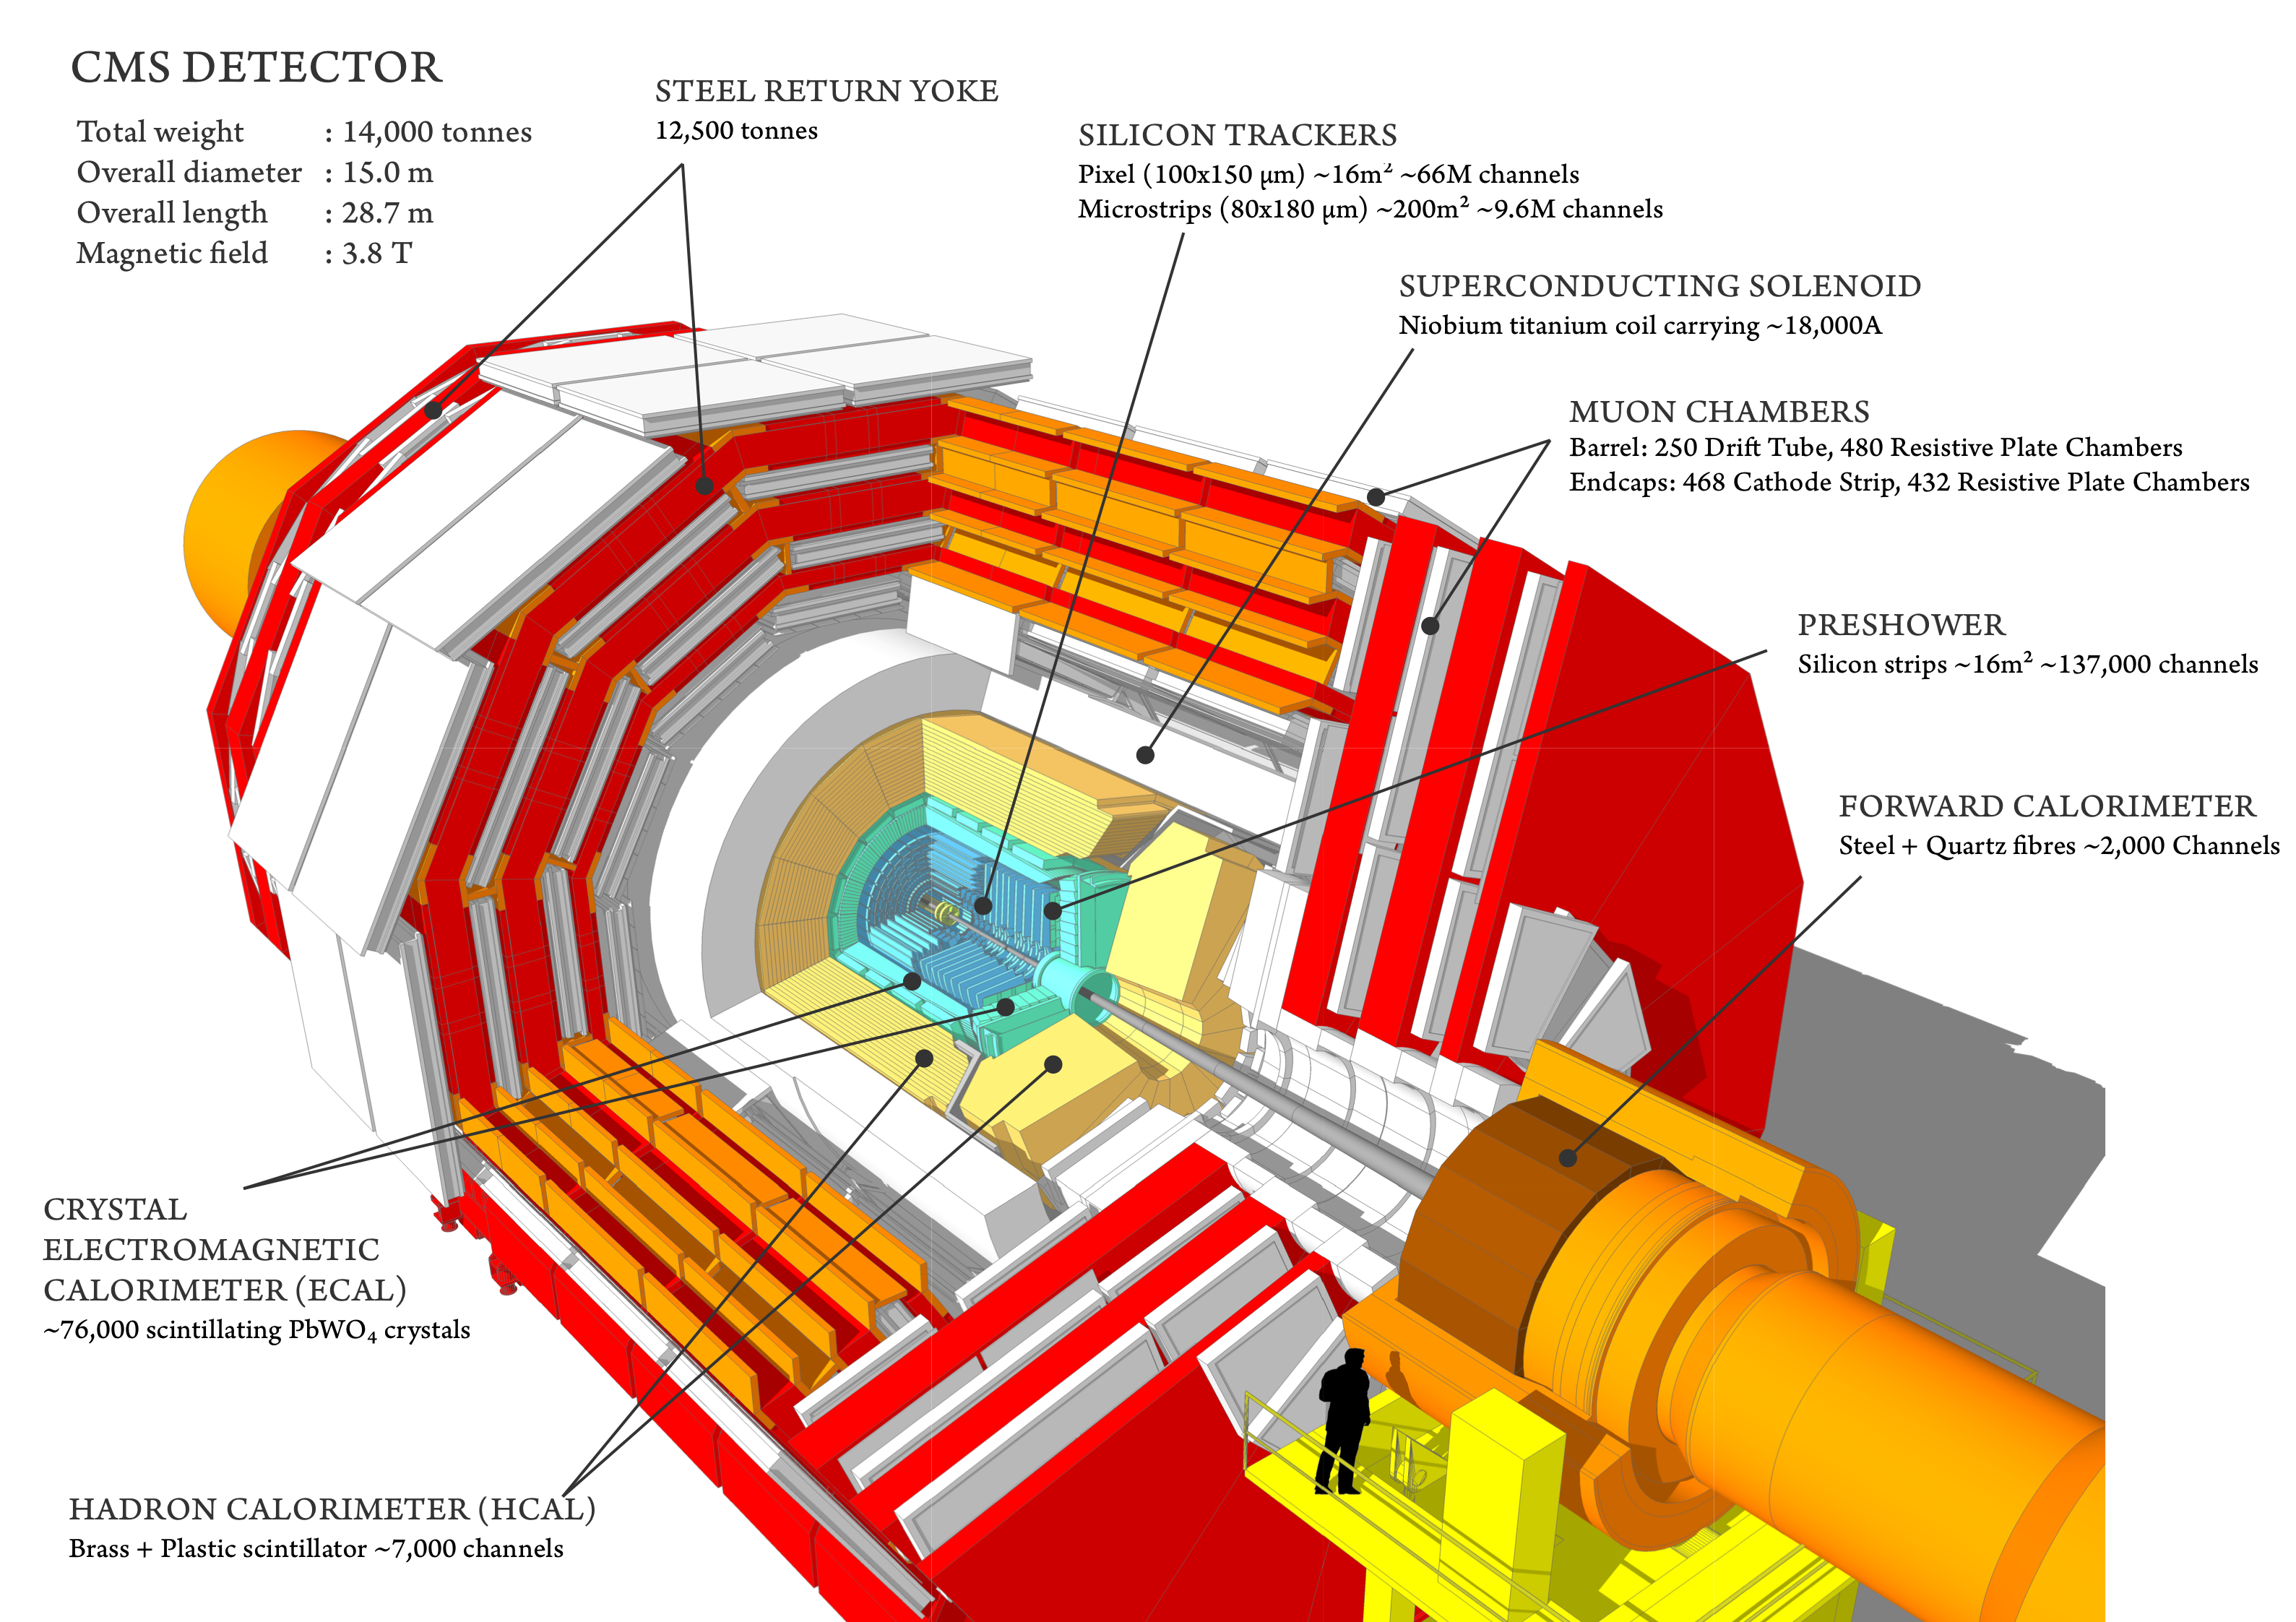
\includegraphics[width=\linewidth]{CMSLayout.png}
\caption{CMS Detector \label{CMSLayout}}
\end{figure}

A property from these particles that is exploited is their charge. Normally, particles produced in collisions travel in a straight line, but in the presence of a magnetic field, their paths are skewed and curved. Except the muon system, the rest of the subdetectors lie inside a 3.8 Tesla magnetic field . Due to the magnetic field the trajectory of charged particle produced in the collisions gets curved  (as shown in \autoref{CMSLayers} ) and one can calculate the particle’s momentum and know the type of charge on the particle.  The Tracking devices are responsible for drawing the trajectory of the particles by using a computer program that reconstructs the path by using electrical signals that are left by the particle as they move.  The Calorimeters measure the energy of particles that pass through them by absorbing their energy with the intent of stopping them. The particle identification detectors work by detecting radiation emitted by charged particles and using this information they can measure the speed, momentum, and mass of a particle. After the information is put together to make the “snapshot” of the collision one looks for results that do not fit the current theories or models in order to look for new physics.

\begin{figure}[h]
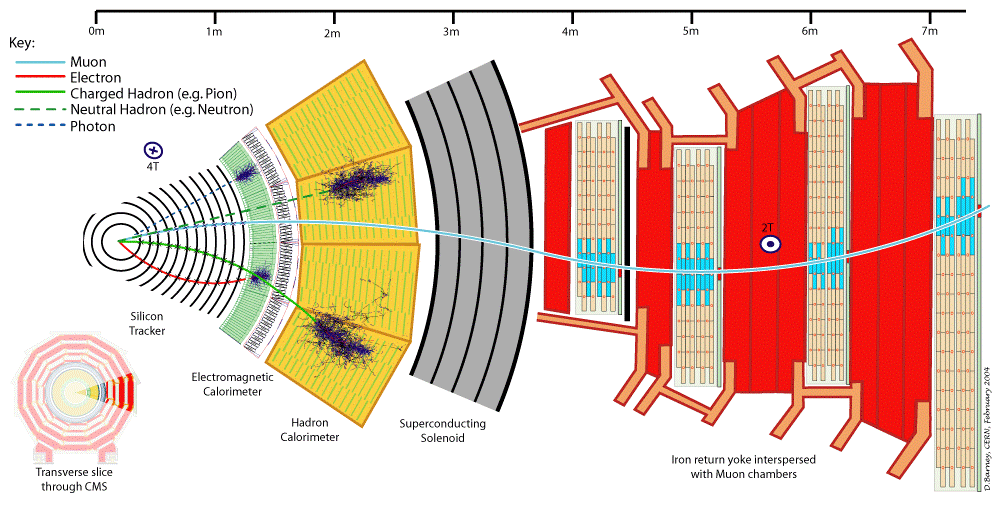
\includegraphics[width=\linewidth]{CMSLayers.PNG}
\caption{The trajectory of a particle traveling through the layers of the detector leaving behind a it's signature footprint\label{CMSLayers}}
\end{figure}


The project focusses specifically on data collected from one of the Calorimeters, - the Hadron Calorimeter (HCAL). The HCAL, as its name indicates, is designed to detect and measure the energy of hadrons or, particles that are composed of quarks and gluons, like protons and neutrons. Additionally, it provides an indirect measurement of the presence of non-interacting, uncharged particles such as neutrinos (missing energy) . Measuring these particles is important as they can tell us if new particles such as the Higgs boson or supersymmetric particles (much heavier versions of the standard particles we know) have been formed. The layers of the HCAL are structured in a staggered fashion to prevent any gaps that a particle might pass through undetected. There are two main parts: the barrel and the end caps. There are 36 barrel wedges that form the last layer of the detector inside the magnet coil, there is another layer outside this, and on the endcaps, there are another 36 wedges to detect particles that come out at shallow angles with respect to the beam line.




\chapter{Data Collection and Data Quality Monitoring \label{DQMchapter} }
%Section 3.1
\section{What is Data Collection for CMS?}

During data taking there are millions of collisions occurring in the center of the detector every second. The data per event is around one million bytes (1 MB), that is produced at a rate of about 600 million events per second \cite{datataking}, that’s about 600 MB/s. Keeping in mind that only certain events are considered “interesting” for analysis, the task of deciding what events to consider out of all the data collected is a two-stage process. First, the events are filtered down to 100 thousand events per second for digital reconstruction and then more specialized algorithms filter the data even more to around 100~200 events per second that are found interesting.
For CMS there is a Data Acquisition System that records the raw data to what’s called a High-Level Trigger farm which is a room full of servers that are dedicated to processing and classify this raw data quickly. The data then gets sent to what’s known as the Tier-0 farm where the full processing and the first reconstruction of the data are done. \cite{cmscomputing} 


\section{What is Data Quality Monitoring?}
To operate a sophisticated and complex apparatus as CMS, a quick online feedback on the quality of the data recorded is needed to avoid taking low quality data and to guarantee a good baseline for the offline analysis. Collecting a good data sets from the collisions is an important step towards search for new physics as deluge of new data poses an extra challenge of processing and storage. This all makes it all the more important to design algorithms and special software to control the quality of the data. This is where the Data Quality Monitoring (DQM) plays a critical in the maintainability of the experiment, the operation efficiency and performs a reliable data certification.  The high-level goal of the system is to discover and pinpoint errors, problems occurring in detector hardware or reconstruction software, early, with sufficient accuracy and clarity to maintain good detector and operation efficiency. The DQM workflow consists of 2 types: \textbf{Online}  and \textbf{Offline}.

The Online DQM consists of receiving data taken from the event and trigger histograms to produce results in the form of monitoring elements like histogram references and quality reports. This live monitoring of each detector’s status during data taking gives the online crew the possibility to identify problems with extremely low latency, minimizing the amount of data that would otherwise be unsuitable for physics analysis. The scrutiny of the Online DQM is a 24/7 job that consists of people or shifters that work at the CMS control center constantly monitoring the hundreds of different plots and histograms produced by the DQM software. This consumes a lot of manpower and is strenuous work. 
The Offline DQM is more focused on the full statistics over the entire run of the experiment and works more on the data certification. In the offline environment, the system is used to review the results of the final data reconstruction on a run-by-run basis, serving as the basis for certified data used across the CMS collaboration in all physics analyses. In addition, the DQM framework is an integral part of the prompt calibration loop. This is a specialized workflow run before the data are reconstructed to compute and validate the most up-to-date set of conditions and calibrations subsequently used during the prompt reconstruction.
This project aims to minimize the DQM scrutiny by eye and automate the process so that there is a more efficient process to monitor the detector and the quality of the data by implementing Machine Learning techniques.



%\begin{comment} %
\begin{figure}[tb]
\begin{center}
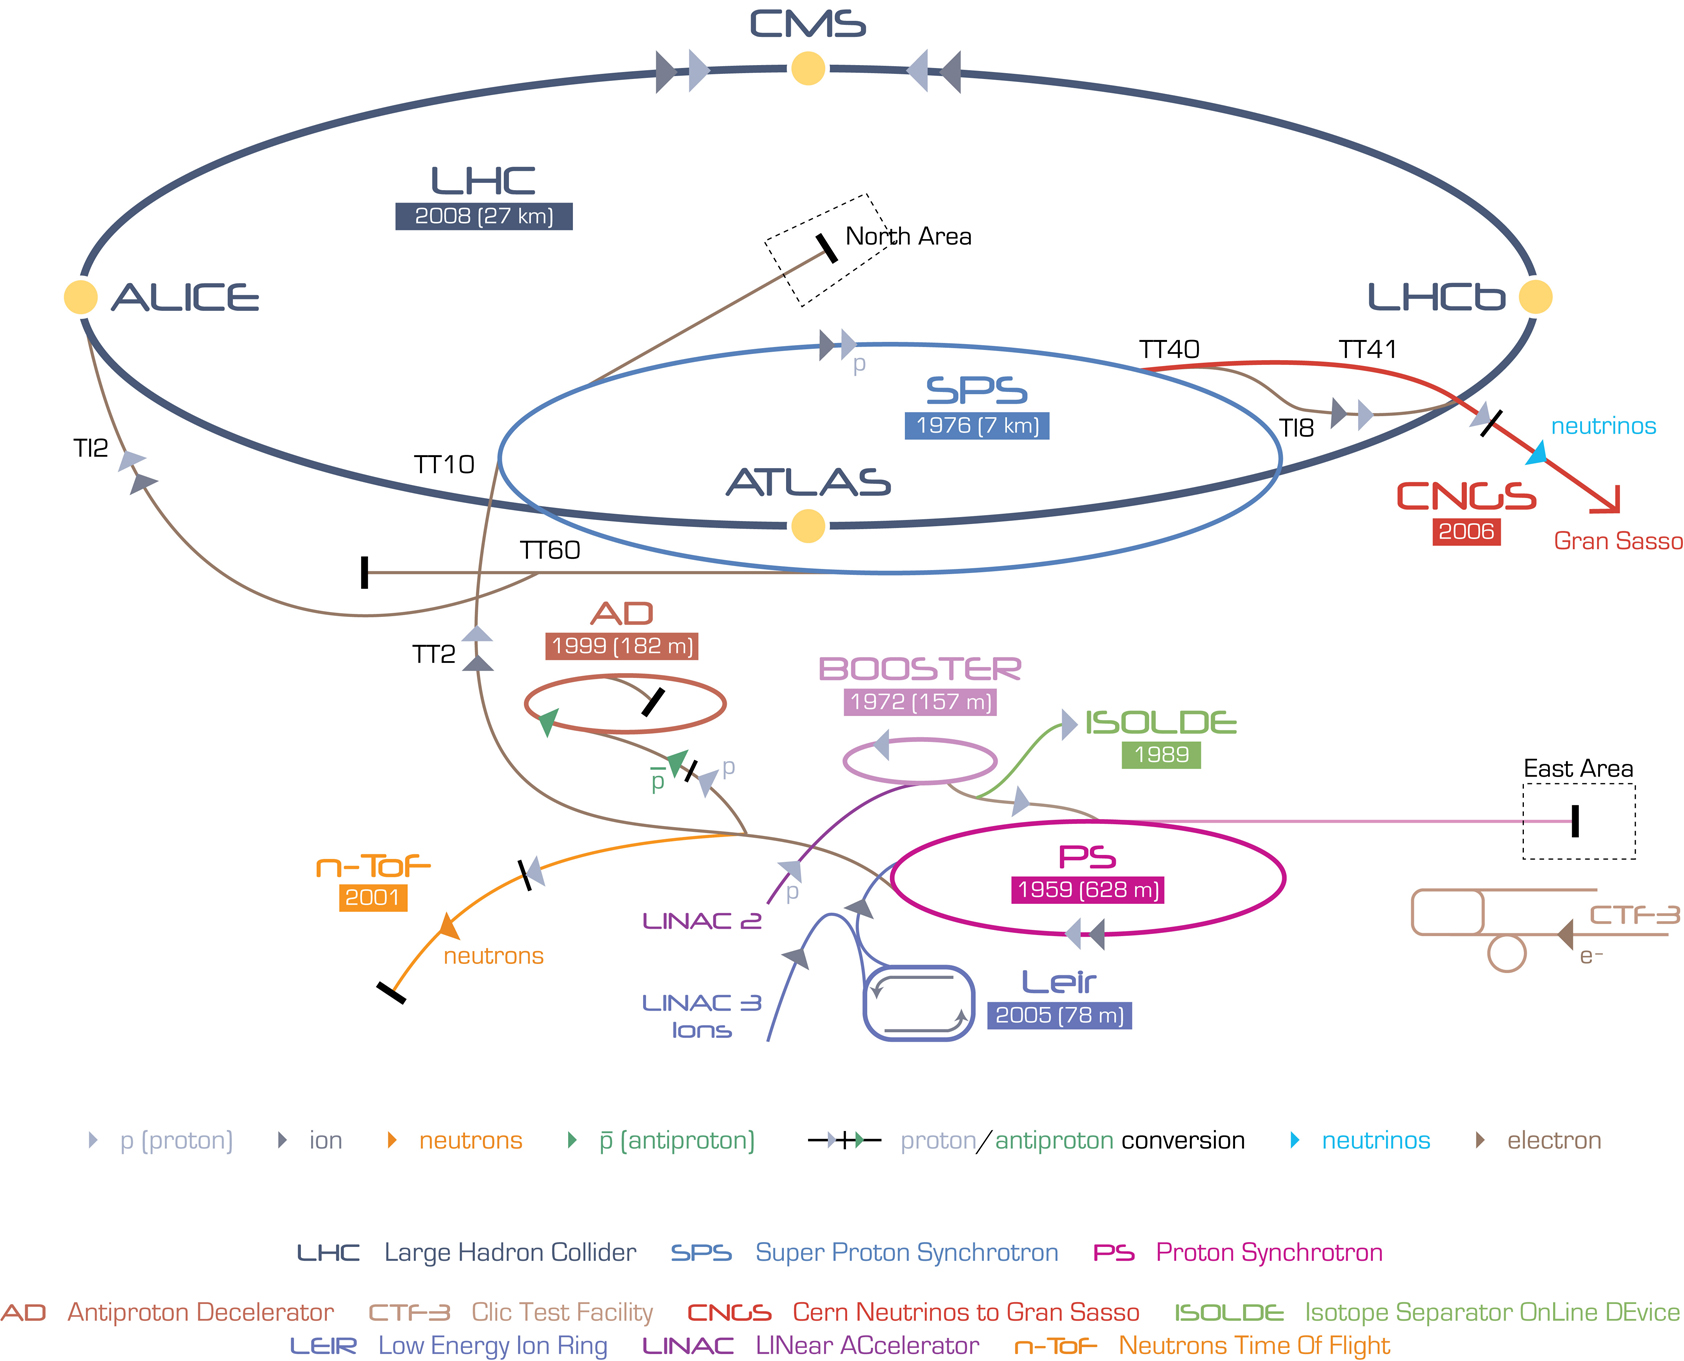
\includegraphics[width=1.0\textwidth]{Cern-Accelerator-Complex.jpg} 
\caption{The CERN Accelerator Complex\cite{LHCcomplex}.}
\label{Cern-Accelerator-Complex.jpg} 
\hspace{4em}
\end{center}
\end{figure}
%\end{comment} %

The four main detectors comprising the LHC machine are CMS, ATLAS\cite{ATLAS}, LHCb\cite{LHCb} and ALICE\cite{ALICE}. Both CMS and ATLAS are general purpose detectors whose initial designs had the detection of the SM Higgs boson, with its wide range of decay modes, in mind. Both detectors managed to accomplish this goal when a 126 GeV scalar boson consistent with the SM Higgs was independently verified by both experiments in July of 2012. Furthermore, the designs for CMS and ATLAS allow for the search of many other additional phenomena in BSM physics such as Supersymmetry, Dark Matter\cite{DM}, Dark Sector\cite{DS}, etc. On the other hand, the LHCb and ALICE detectors focus on more particular kinds of searches. The main motivation for the LHCb experiment, where the b stands for beauty, concerns itself with the measurement of CP violation parameters in b-hadron interactions and studies cover a wide range of aspects of Heavy Flavor Electroweak and QCD physics. Meanwhile, the ALICE experiment focuses on the study of heavy ion (Pb-Pb) nuclei collisions at a centre-of-mass energy of 2.76 TeV in order to better understand the physics behind strongly interacting matter at extreme energy densities.

%Section 3.2
\section{The CMS Detector}
The Compact Muon Solenoid (CMS) detector is a general purpose particle detector designed to investigate various physical phenomena concerning the SM and beyond it, such as Supersymmetry, Extra Dimensions and Dark Matter. As its name implies, the detector is a solenoid which is constructed around a superconducting magnet capable of producing a magnetic field of 3.8 T. The magnetic coil is 13m long with an inner diameter of 6m, making it the largest superconducting magnet ever constructed. The CMS detector itself is 21m long with a diameter of 15m and it has a weight of approximately 14,000 tonnes. The CMS experiment is one of the largest scientific collaborations in the history of mankind with over 4,000 participants from 42 countries and 182 institutions.\\

%\begin{comment} %
\begin{figure}[tb]
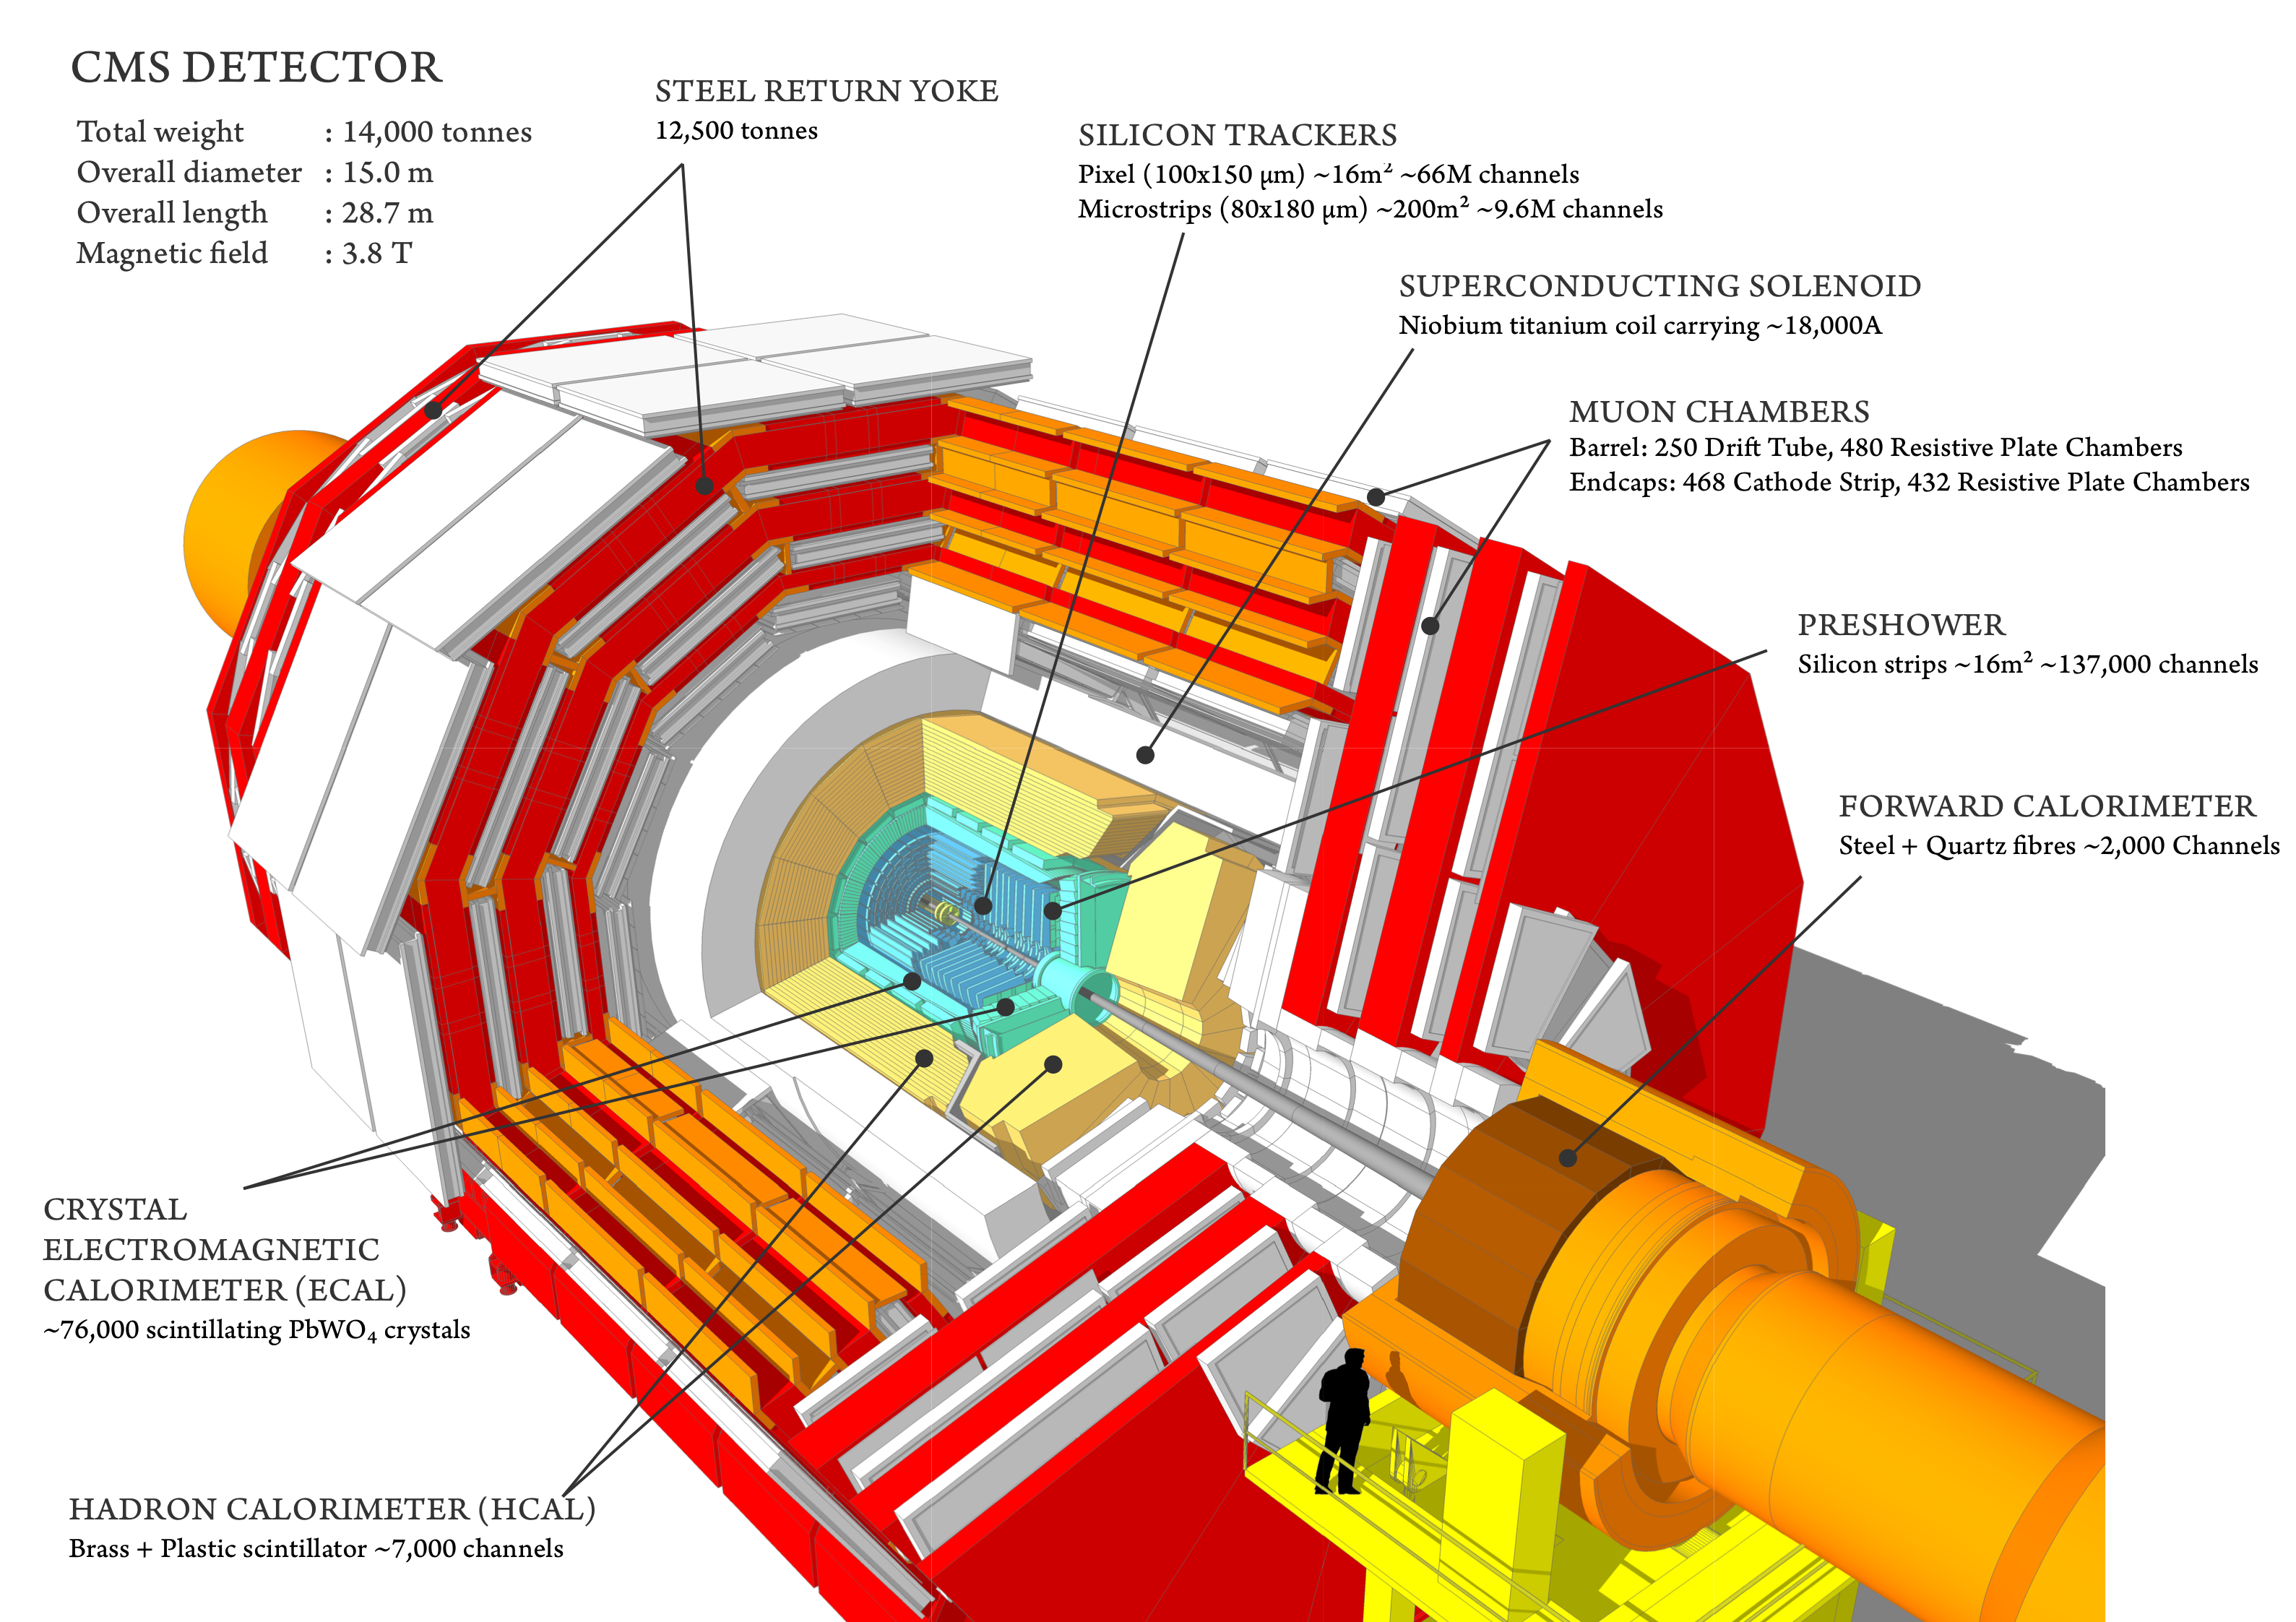
\includegraphics[width=1.0\textwidth]{CMSLayout.png} 
\caption{The CMS Detector Layout\cite{CMSlayout}.}
\label{CMSLayout} 
\hspace{4em}
\end{figure}
%\end{comment} %

In order to meet the many needs of the SM and BSM searches, and the goals of the LHC physics program, the CMS detector was designed with the following features:\\
\begin{itemize}
	\itemsep-1em
	\item{A magnet with large bending power and high performance muon detector for good muon identification and momentum resolution over a wide range of momenta and angles.}\\
	\item{An inner tracking system capable of high reconstruction efficiency and momentum resolution requiring pixel detectors close to the interaction region.}\\
	\item{An electromagnetic calorimeter able to provide good electromagnetic energy resolution and a high isolation efficiency for photons and leptons.}\\
	\item{A hadron calorimeter capable of providing precise missing-transverse-energy ($p_\text{T}^{miss}$)  and dijet-mass resolution.}\\
\end{itemize}

A general layout of the CMS detector and all its constituent sub-detectors can be seen in \autoref{CMSLayout}. The configuration of the CMS sub-detectors follow a cylindrical layer pattern that is symmetrical about the interaction region and consists of a central barrel with endcaps on both ends.

The coordinate system for the CMS detector design uses a right-hand rule convention centered around the ideal interaction point to describe the positions of objects in the experiment. The z-axis is defined along the direction of the LHC beam, with the x-axis pointing towards the center of the LHC ring. In terms of polar coordinates then, r is the radial distance from the center of the pipe, the polar angle $\theta$ is measured against the z-axis and the azimuthal angle $\phi$ is measured with respect to the x-axis. However, the pseudorapidity $\eta$ is generally preferred over the polar angle $\theta$. The pseudorapidity is defined as:

\begin{center}
$\eta$ =  $-$ ln tan $\frac{\theta}{2}$.
\end{center}

\subsection{Silicon Tracking System}

The CMS tracking system was designed with the goal of obtaining precise and efficient measurements for the trajectories of charged particles resulting from proton-proton collisions at the LHC. 
In addition, it allows for the precise measurement of secondary vertices and impact parameters needed to efficiently identify the heavy flavours produced in many interesting physics channels. Due to the LHC's design Luminosity of 10$^{34}$ cm$^{-2}$s$^{-1}$, the currently installed CMS phase-1 tracker is expected to handle an average of 1000 particles from over 20 overlapping proton-proton interactions per bunch crossing, every 25 ns. This required a detector technology capable of achieving a high granularity and fast response as well as being tolerant to the radiation produced from the intense particle flux. These considerations lead to a tracker design composed entirely of silicon detector technology which features an active silicon area of about 200 m$^2$, making it the largest silicon tracker ever built\cite{CMSdet1}.\\

%\begin{comment} %
\begin{figure}[tb]
\begin{center}
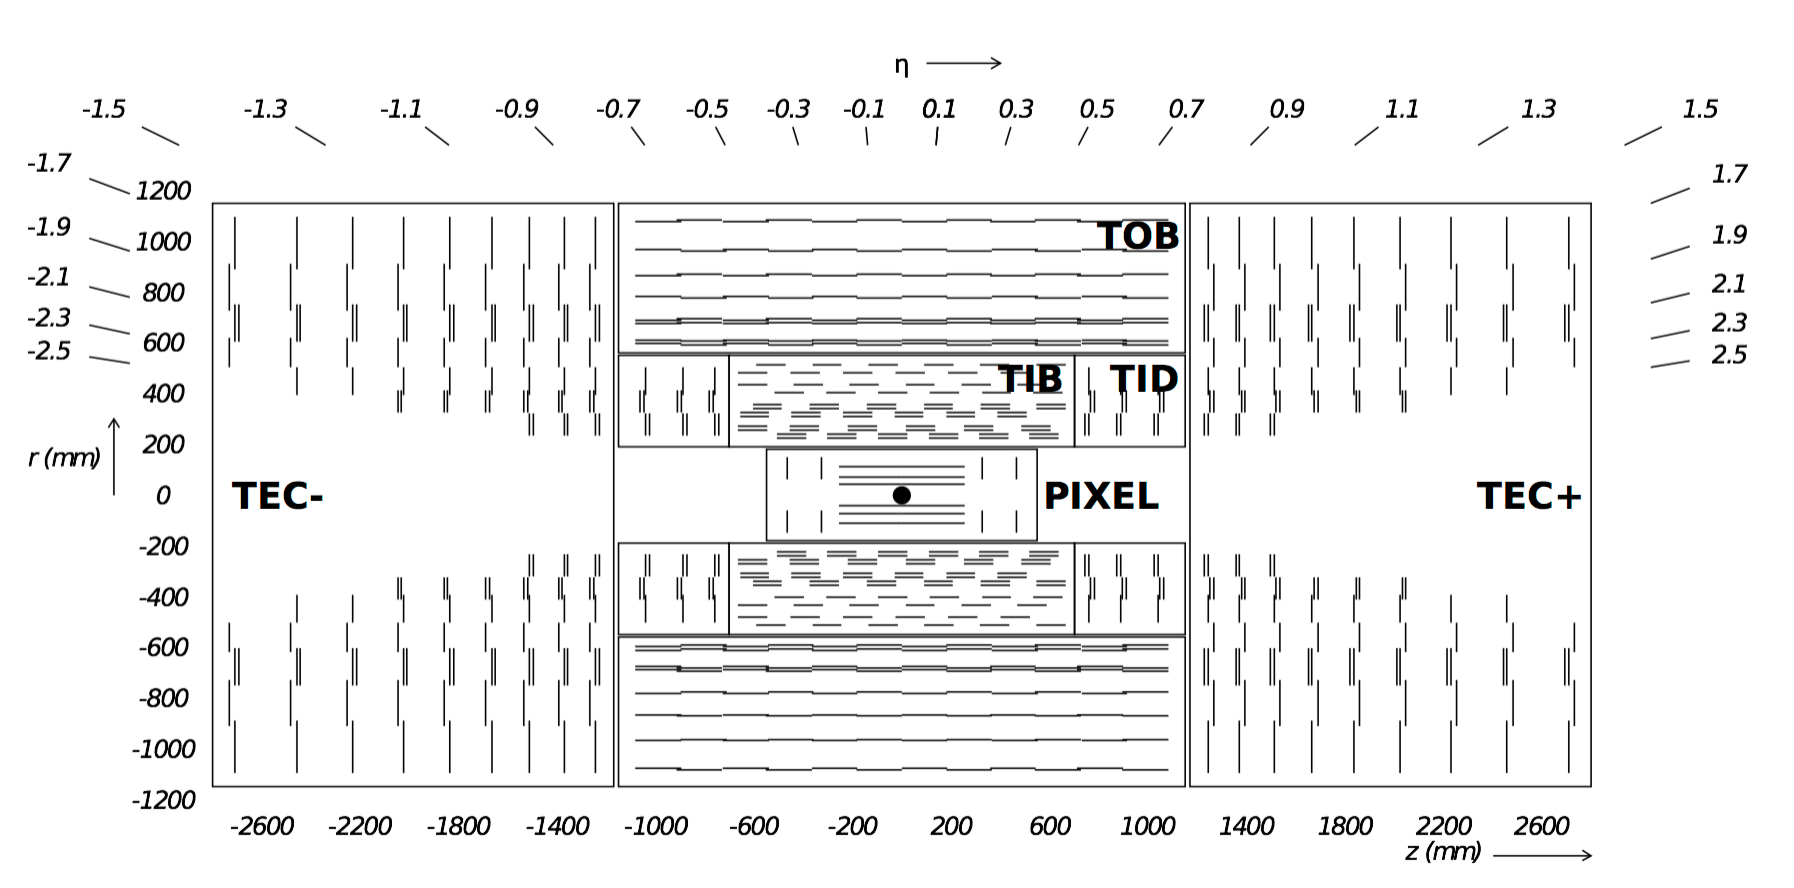
\includegraphics[width=0.9\textwidth]{CMSTrackerLayout.png} 
\caption{Overview of the CMS Tracker Layout\cite{CMSdet2}.}
\label{CMSTrackerLayout} 
%\hspace{4em}
\end{center}
\end{figure}
%\end{comment} %

The CMS tracker is built in a cylindrical manner around the interaction point and has a diameter of 2.5 m and a length of 5.8 m. It is comprised of a pixel detector with three barrel layers, positioned at a distance between 4.4 cm and 10.2 cm from the interaction region, and a silicon strip tracker with 10 barrel detection layers extending to a radius of 1.1 m. Each system is made complete by endcaps at opposite sides of the barrel, consisting of 2 discs for the pixel detector and 3 plus 9 discs for the strip tracker, extending the acceptance region of the tracker up to a pseudorapidity $|\eta| <$ 2.5.\\

The pixel detector is the part of the CMS tracking system closest to the interaction region and consists of 3 barrel layers (BPix) and 2 endcap discs (FPix). It is responsible for providing precise tracking points in $r$-$\phi$ and $z$, a feature that is required for the small impact parameter resolution, needed for good secondary vertex reconstruction. The detector contains 1440 modules covering an area of approximately 1 m$^2$ making up a total of 66 million pixels. The sensors were designed using an n-on-n concept from 320 $\mu$m thick silicon wafers and are fabricated with read-out chips (ROCs) that are bump-bonded to the sensor in standard 0.25 $\mu$m CMOS technology. Each of the pixels has a pitch size of 100 $\times$ 150 $\mu$m$^2$, which corresponds to an occupancy of about 10$^{-4}$ per bunch crossing.\\

The silicon strip tracker is built surrounding the pixel detector and consists of three large subsystems. The Tracker Inner Barrel and Disks (TIB/TID) extend to a radius of 55 cm and are composed of four barrel layers, completed by three disks at each end. The TIB/TID employs the use of 320 $\mu$m thick silicon micro-strip sensors in order to deliver up to 4 $r$-$\phi$ measurements on a trajectory. Surrounding the TIB/TID is the Tracker Outer Barrel (TOB), which consists of 6 barrel layers and has an outer radius of 116 cm. The TOB extends symmetrically in $z$ between $\pm$118 cm and provides an additional 6 $r$-$\phi$ measurements for a trajectory. Beyond the TOB's $z$ range lie the Tracker Endcaps (TEC+ and TEC-, where the sign indicates their position respect to $z$). Each TEC consists of 9 discs with up to 7 rings of silicon micro-strip detectors, providing up to 9 additional $\phi$ measurements per trajectory. The CMS silicon strip tracker has a total active silicon area of 198 m$^2$ and is composed of 15,148 sensor modules.

\subsection{Electromagnetic Calorimeter}
The CMS Electromagnetic Calorimeter (ECAL) is a hermetic homogeneous calorimeter whose function is to measure the energy of particles that interact via the electromagnetic force. With the use of 75,848 scintillator crystals, it is capable of providing good energy resolution within the requirements of the ambitious LHC program. In particular, the ECAL's design was optimized to search for diphoton events resulting from Higgs boson decays (H $\rightarrow \gamma \gamma$).\\ 

%\begin{comment} %
\begin{figure}[tb]
\begin{center}
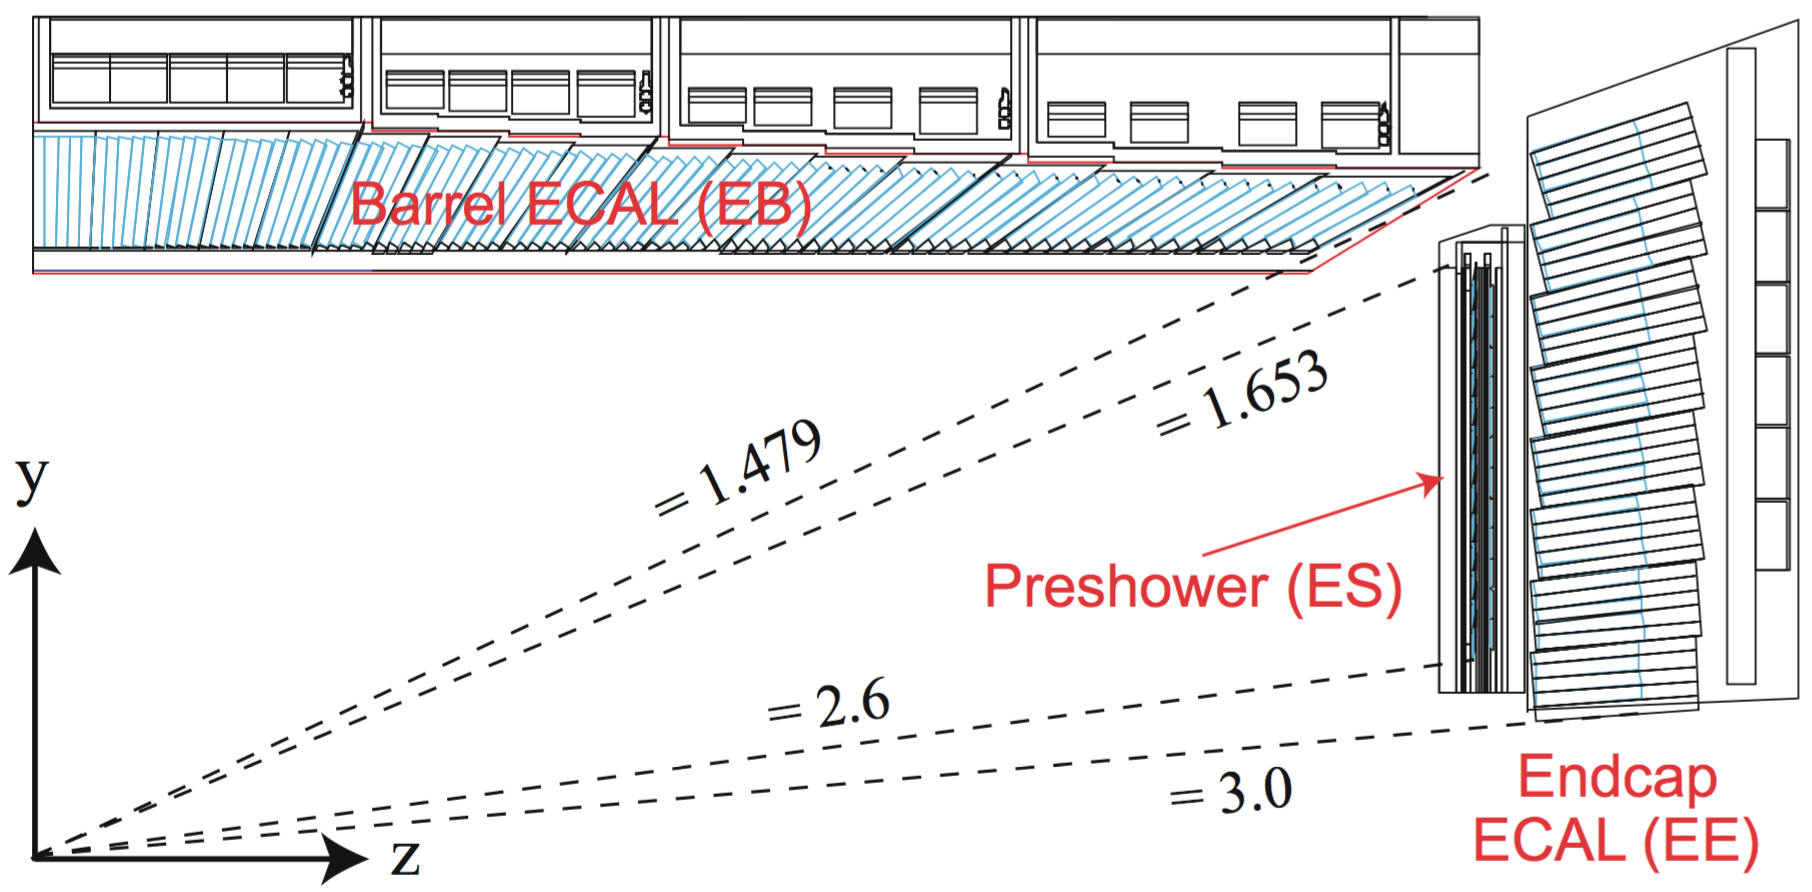
\includegraphics[width=0.8\textwidth]{ECALgeometry.png} 
\caption{Geometrical layout of the CMS Electromagnetic Calorimeter\cite{CMSLHC}.}
\label{CMS_ECAL_Geometry} 
\hspace{4em}
\end{center}
\end{figure}
%\end{comment} %

The ECAL is composed of two main sub-systems -- the barrel calorimeter (EB) and the endcap calorimeter (EE) -- and is completed by a preshower calorimeter (ES), as shown in \autoref{CMS_ECAL_Layout}. It covers a solid angle up to a pseudorapidity of $|\eta| <$ 3, with the EB extending in the range of $|\eta| <$ 1.479 and the EE covering a range of  1.479 $< |\eta| <$ 3. Both subsystems are composed of lead tungstate (PbWO$_4$) scintillator crystals which provide a fast response time and high radiation tolerance, both crucial requirements for optimal performance at LHC operating conditions. In addition, the properties of the PbWO$_4$ crystals (high density, short radiation and small Moli\'ere radius) led to the design of a compact calorimeter with fine granularity.\\

The barrel part of the ECAL (EB) is composed of specially designed avalanche photodiodes (APD). It consists of 61,200 crystals, forming a total volume of 8.14 m$^3$ and weighing about 67.4 t. The crystals that form the EB are 230 mm long with a cross-section of 22$\times$22 mm$^2$ at the front face and 26$\times$26 mm$^2$ at the back. They are organized in pairs within thin-walled alveolar structures called submodules. The submodules are assembled into different types of modules that differ by their location with respect to $\eta$ and contain 400 or 500 crystals each. Theses modules are then arranged in sets of four modules, called supermodules, and contain 1700 crystals each. Thus, the EB is composed of two half-barrels, each consisting of 18 supermodules.\\

In contrast, the photodetectors used in the endcap section of the ECAL are vacuum phototriodes (VPT)\cite{VPT}. Each of the endcaps contain 7,324 crystals which, in total, occupy a volume of 2.90 m$^3$ and weigh about 24.0 t. The crystals in the EE are 220 mm in length with a cross-section of 28.62$\times$28.62 mm$^2$ for the front face and 30$\times$30 mm$^2$ in the rear. They are all identical in shape and are arranged in mechanical units of 5$\times$5 crystals, called supercrystals (SC), which consist of carbon-fibre alveola structures. Each of the endcaps are divided into two semi-circular structures, called \textit{Dees}, which hold a total of 3,662 crystals. \\

The ES preshower is located before the EE detector and spans a pseudorapidity range of 1.653 $< |\eta| <$ 2.6. It's main purpose is to identify neutral pions in the endcaps as well as to improve the determination of electrons and photons with high granularity. The preshower consists of two layers and has a total thickness of 20 cm. The first layer is conformed by lead radiators which initiate electromagnetic showers from incoming photons and electrons. Meanwhile, the second layer is composed of silicon strips which are capable of measuring the deposited energy and the transverse shower profiles.

%\begin{comment} %
\begin{figure}[tb]
\begin{center}
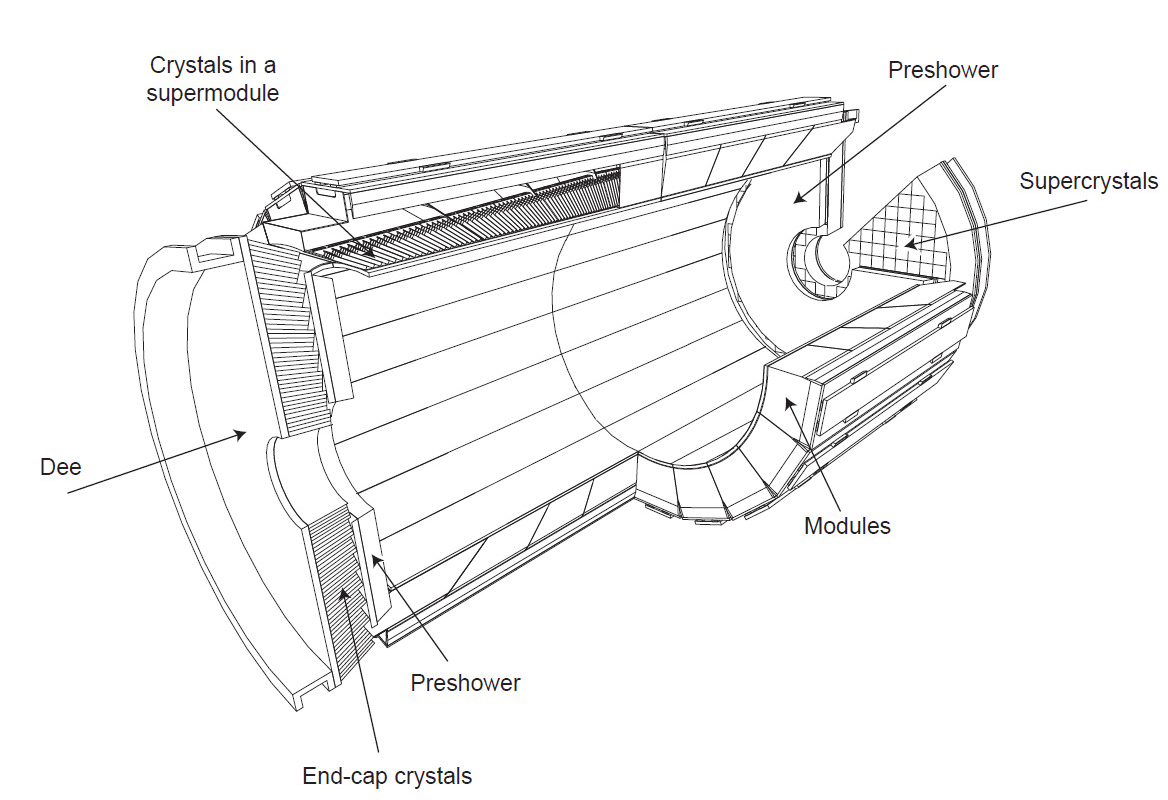
\includegraphics[width=0.9\textwidth]{ECALlayout.png} 
\caption{Layout of the CMS ECAL illustrating its various components\cite{CMSdet1}.}
\label{CMS_ECAL_Layout}
\vspace{-1em}
\end{center}
\end{figure}
%\end{comment} %

\subsection{Hadron Calorimeter}

The CMS Hadron calorimeter (HCAL) conforms the next layer of the CMS detector. It is a sampling calorimeter that consists of alternating layers of massive absorbing brass plates and plastic scintillator tiles and is of particular importance for the measurement of hadron jet energy and  $p_\text{T}^{miss}$. The HCAL detector is located in between the outer extent of the ECAL ($R$ = 1.77 m) and the inner extent of the magnet coil ($R$ = 2.95 m). Similar to the other CMS subsystems, it's composed of a barrel part (HB) and an endcap part (HE). In addition, it features a tail-catching outer calorimeter (HO), located outside the magnet, and a forward calorimeter (HF) in the very forward region near the beam line. A layout of the HCAL system can be seen in \autoref{CMS_HCAL_Layout}.\\

%\begin{comment} %
\begin{figure}[tb]
\begin{center}
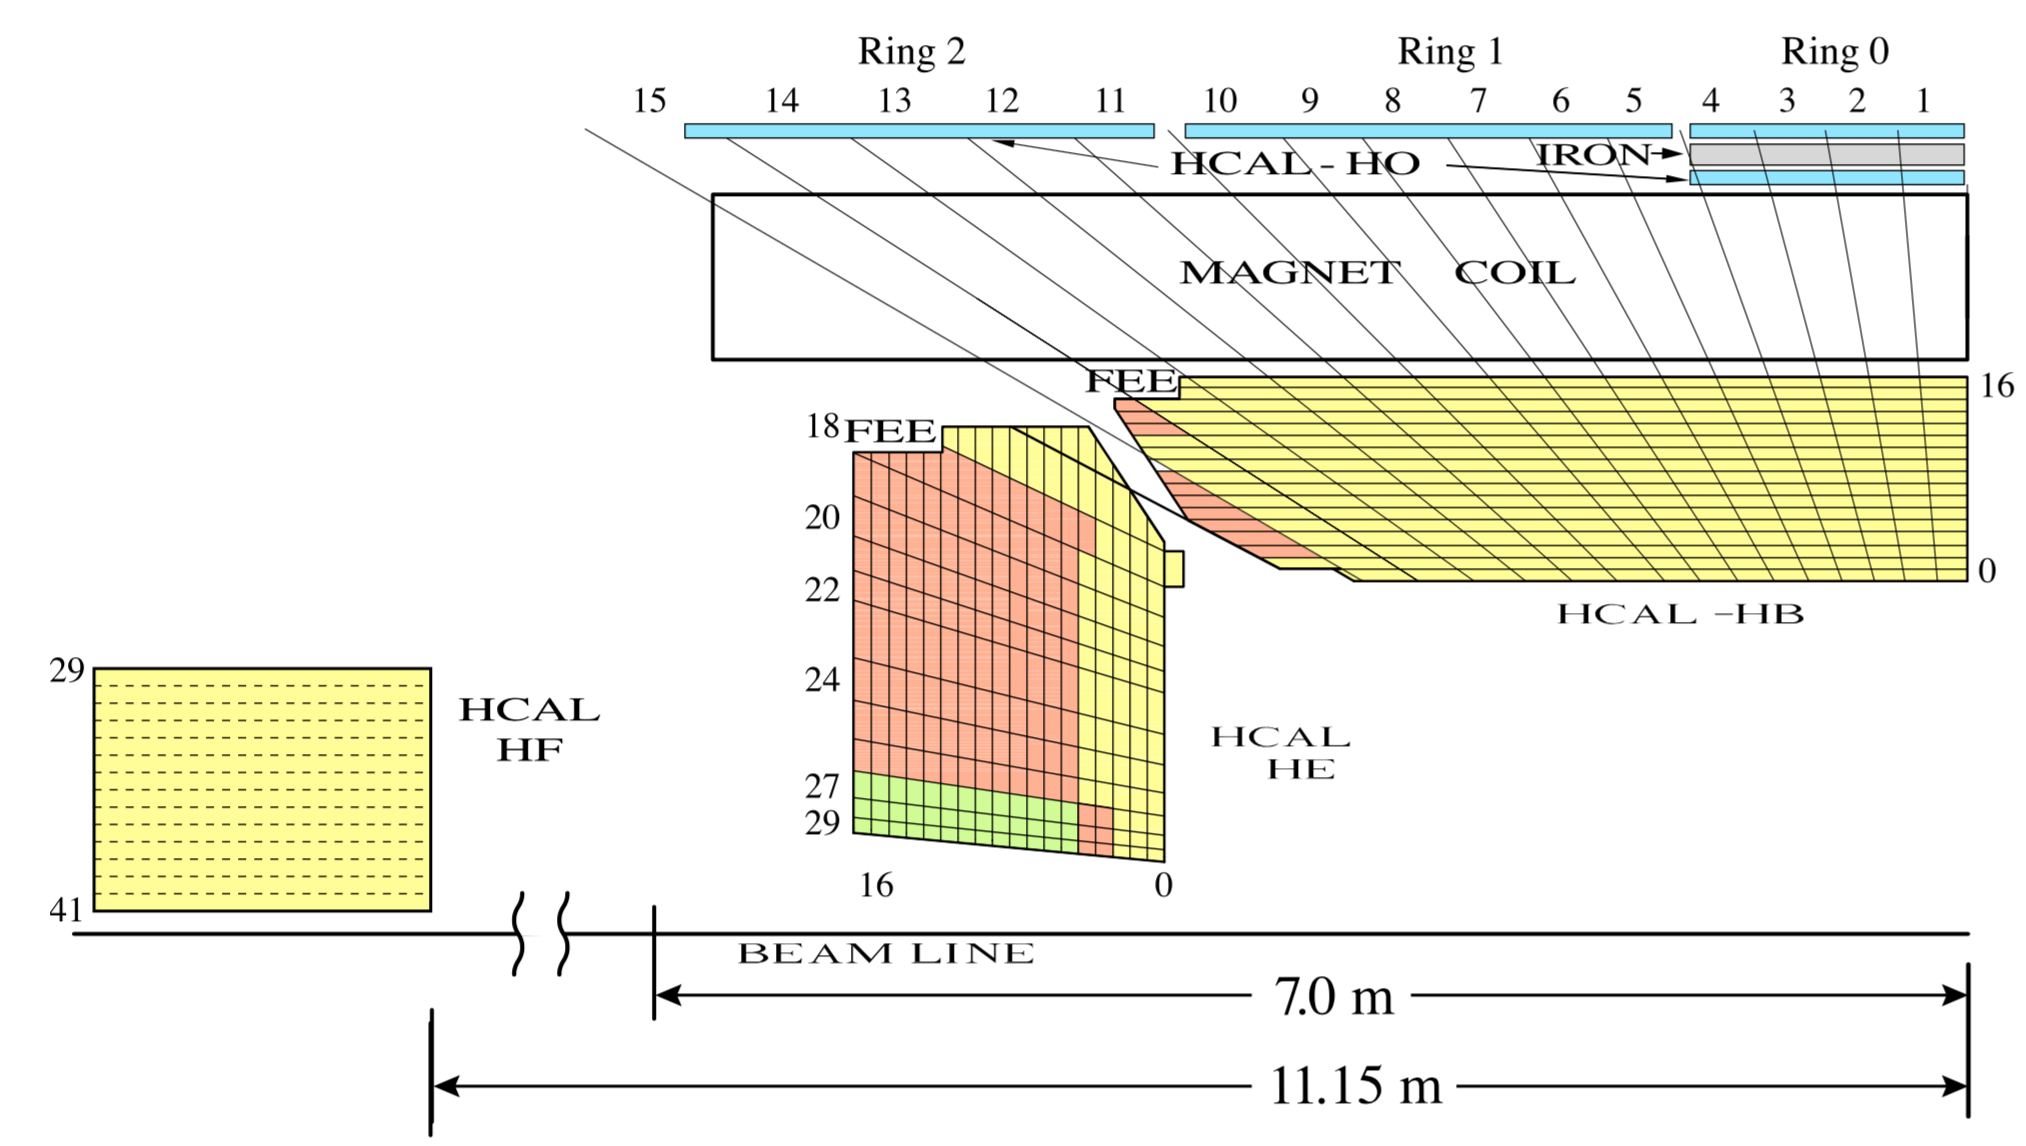
\includegraphics[width=0.9\textwidth]{CMS_HCAL.png} 
\caption{Geometrical layout of the HCAL showing the locations of the hadron barrel (HB), endcap (HE), outer (HO) and forward (HF) calorimeters\cite{CMShcal}.}
\label{CMS_HCAL_Layout} 
\end{center}
\end{figure}
%\end{comment} %

The barrel component of the HCAL is a sampling calorimeter which covers the pseudorapidity range $|\eta|<$1.3. It consists of both the HB and the HO detectors. The reason behind separating the barrel detector into the HB and HO is due to the limited amount of space available for the barrel detector. The HB is located within the superconducting magnet coil and is supplemented by the HO in between the outer solenoid coil and the muon chambers. Therefore, the HO acts as a tail-catcher in order to improve the jet energy measurements and $p_\text{T}^{miss}$, with the solenoid in between acting as absorber material. The HB consists of two half-barrel sections, identified as HB+ and HB- due to their geometrical location, which are composed of 36 identical azimuthal wedges. The wedges, which are constructed out of flat brass absorber plates, are aligned parallel to the beam axis and are segmented into four azimuthal angle ($\phi$) sections.\\ 

The HE covers a significant amount of the pseudorapidity in the range of 1.3 $< |\eta| <$ 3, a region containing about 34\% of the particles produced in the final state. Due to the high luminosity of the LHC, the HE is required to have a high radiation tolerance at $|\eta| \simeq 3$, as well as being capable of handling high counting rates. Similar to the HB, the HE is also composed of brass absorber plates and scintillator plates which are read out by wavelength shifting fibers. The light captured by the scintillators merges within the wavelength shifting fibers and then it's read out by hybrid photo-diodes. The scintillators are partitioned in towers with an area of $\Delta\eta\times\Delta\phi = 0.17\times0.17$.\\

\subsection{Magnet}

The CMS superconducting solenoid is one of the driving features of the detector design. It is capable of providing a magnetic field with a 3.8T magnitude, which allows for the large bending power needed for  precise particle transverse momentum ($p_{\text{T}}$) measurements. The magnet is made of four layers of stabilized reinforced Niobium-Titanium (NbTi) and has a cold mass of 220 t. The solenoid consists of a 13 m long coil with an internal diameter of 6 m, which houses both the tracking and calorimetric system. This design allows for particles to be measured prior to crossing the magnetic coil which significantly improves the energy resolution. 

\subsection{Muon Detector}

 As implied by the detector's name, precise and robust muon measurements have been a central theme of the CMS experiment since the early stages of its design. The detector design takes into account that muons behave as minimum ionizing particles (MIPs)\cite{MIPs} and can therefore manage to traverse
the tracker and calorimeters with minimal energy loss. Furthermore, due to their relatively long lifetime they can be efficiently identified by a dedicated system at the outer region of the detector. Consequently, the CMS muon systems comprise the outermost layer of the detector, which are integrated into the magnet return yoke that surrounds the solenoid.\\

The muon system is capable of three main functions: muon identification, muon $p_{\text{T}}$ measurement and triggering. It is composed of three different types of detectors, all of which make use of gaseous chamber technology. This choice of detector provides a cost efficient way of covering most of the full solid angle, featuring a total of 25,000 m$^2$ of detection plates. As a consequence of the shape of the solenoid magnet, the muon detector was designed to have a cylindrical barrel section as well as two planar endcap regions.\\

\begin{figure}[H]
\begin{center}
\begin{minipage}[b]{0.59\textwidth}
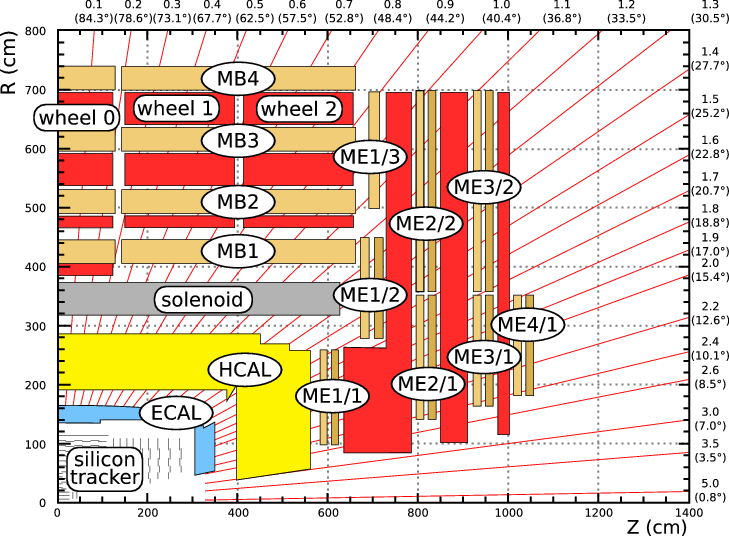
\includegraphics[width=\textwidth]{muonAlignment.png}
\end{minipage}
\hspace{1em}
\begin{minipage}[b]{0.3\textwidth}
    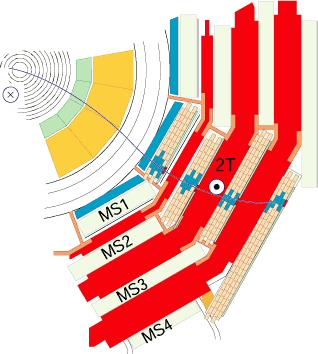
\includegraphics[width=\textwidth]{MuStations.png}
\end{minipage}
\end{center}
\vspace{-1em}
\caption[Quarter-view of the CMS muon system (left) and a muon in the transverse plane leaves a curved trajectory across the four muon detector stations (right).]{The left diagram shows a quarter-view of CMS with both the muon barrel (MB) and endcap (ME) stations \cite{muonAlignment}.  The right diagram shows a muon in the transverse plane leaves a curved trajectory across the four muon detector stations\cite{MuDet}.}
\label{muonSystem}
\end{figure}

For the barrel region of the muon detector, four layers of drift tube (DT) modules are used, covering a pseudorapidity of up to $|\eta| < 1.2$. These four layers, called ``stations'', are arranged in cylindrical concentric layers around the beam line, where the first three layers have 60 DTs each and the outer cylinder has 70. Each of the DT stations contain 12 individual gas filled tubes, all of which have a 4cm diameter and a center electrode. The use of DTs as tracking detectors for the barrel muon system is possible because of the low expected muon rate and the relatively low strength of the local magnetic field.\\
 
The endcap regions of the muon system are subject to a higher muon rate, and cover the range $0.9 < |\eta| < 2.4$ where the magnetic field is stronger and less homogeneous. Considering these conditions, cathode strip chambers (CSCs) are employed, which feature high granularity, fast response time and adequate radiation hardness. CSCs consist of arrays of positively-charged ``anode'' wires crossed with negatively-charged copper ``cathode'' strips within a gas volume. They are trapezoidal in shape and can cover either $\ang{10}$ or $\ang{20}$ in $\phi$. Furthermore, CSCs have the advantage of featuring both precision muon measurement and muon trigger in a single device.\\

The third type of detector used in the CMS muon system are called resistive plate chambers (RPCs) and can be found in both the barrel and endcap regions. They consist of gaseous parallel-plate detectors capable of providing precise timing information and adequate spatial resolution. Because of their excellent time resolution, RPCs provide the capability of tagging the time of an ionizing event between 2 consecutive LHC bunch crossings (BX) in a much shorter time ($\sim$ 1 ns) than the interval between the BXs (25 ns). For this reason, an RPC-based dedicated muon trigger device can be implemented to unambiguously identify the relevant BX to which a muon track is associated with, despite the high rate of events and background expected at the LHC.

\subsection{Trigger and Data Acquisition}

Due to the vast volume of data originating from the proton-proton collisions (delivered by the LHC at a rate of 40 MHz), a method of eliminating the majority of the uninteresting/unwanted events was a requisite for the CMS detector design. This event rate reduction is achieved by the implementation of the so-called trigger system, which manages to select the potentially interesting interactions and reduce the rate from a staggering 40 TBs$^{-1}$ to a manageable value of just a few hundred Hz.\\

The CMS trigger system is implemented using a two-stage rate reduction, which combines both a hardware and software phase. The combination of both of these triggers is designed to reduce the rate by a factor of $\sim10^6$. The first stage used in the rate reduction is purely hardware based and it is called the Level 1 (L1) Trigger \cite{L1T}, which consists of both Field Programmable Gate Array (FPGA) and Application Specific Integrated Circuit (ASIC) technology. During this initial stage, the rate is reduced to about 100 kHz with a latency of 3.2 ${\mu}$s. This time interval constrains the trigger decision, allowing only for data from the calorimeters and muon system to be processed. Trigger primitives (TP) from these subsystems are processed through a series of steps before the combined event information is evaluated by the global trigger (GT) where the final decision, whether or not to accept the event, is made.\\

The second stage, which implements offline-quality reconstruction algorithms in its event selection, is referred to as the High-Level Trigger (HLT)\cite{HLT}. The event selection process for the HLT requires that physics objects for each event, such as electrons, muons and jets, are reconstructed and undergo predetermined identification criteria. 

\subsection{Event Reconstruction}

In order to reconstruct the events the particle flow (PF) algorithm\cite{PFref} is used. This algorithm gathers information from all the CMS sub-detectors to reconstruct charged and neutral hadrons, photons, muons, and electrons. It relies on an efficient and pure track reconstruction, a clustering algorithm able to distinguish overlapping tracks originated from different vertices, and an efficient link procedure to associate each particle deposit in the sub-detectors. Once all the deposits of a particle are associated, it can be correctly identified and its four-momentum optimally determined from the combined information of the sub-detectors. The resulting list of particles are then used to reconstruct higher level objects such as jets, taus, missing transverse energy, and to compute charged lepton and photon isolation, etc\cite{Reco1}. The CMS experiment is provided with millions of collisions per second, which need to be triggered, detected, stored and analyzed in a collaboration of several thousand physicists. This huge amount of data and the complexity of the detector require a flexible data model that serves all the needs of the collaboration. The data format is optimized for performance and flexibility of the reconstruction for the end user's analysis.\\

\begin{figure}[tb]
\begin{center}
%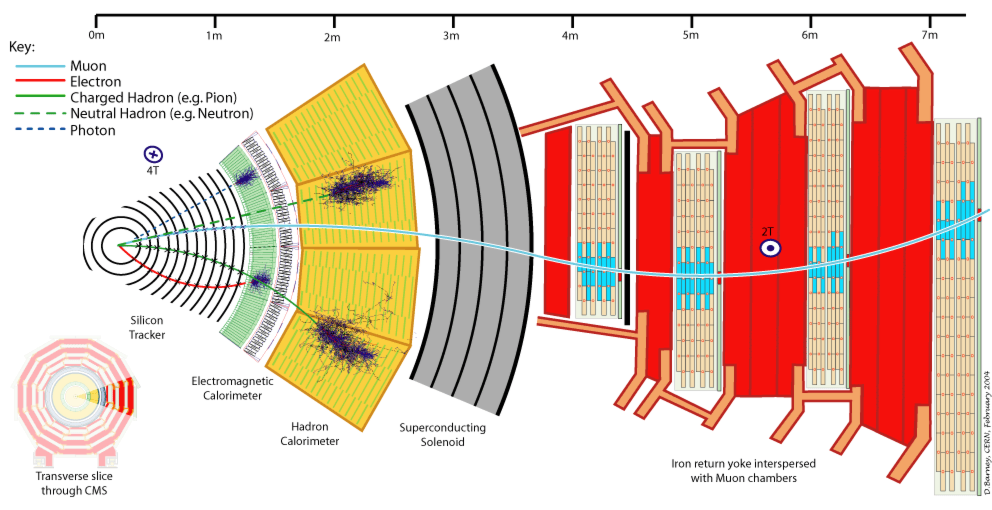
\includegraphics[width=1.0\textwidth]{CMSParticleDet.png} 
\caption{Transverse slice of the CMS detector, showing the individual detector subsystems and particle signatures in each. The particle type can be inferred by combining the detector response in the different subdetectors\cite{CMSslice}.}
\label{CMSParticleDet} 
\end{center}
\end{figure}

Event information from each step in the simulation and reconstruction chain is logically grouped into what is called a data tier\cite{CMScomp1}. From the physicist's point of view the most important data tiers are RECO, which contains all reconstructed objects and hits, and AOD (a subset of RECO). The AOD will contain a copy of all the high-level physics objects (such as muons, electrons, taus, etc.) and enough information about the event to support all the typical usage patterns of a physics analysis. It also contains a summary of the RECO information sufficient to support typical analysis actions such as track refitting with improved alignment or kinematic constraints, re-evaluation of energy and/or position of ECAL clusters based on analysis-specific corrections. The format of each data tier is ROOT \cite{ROOT}. ROOT is a framework for data processing developed at CERN with the sole purpose of aiding high energy physics research. The various AOD datasets are stored worldwide at various data tier centers. From the AOD's the analysis groups create data structures called NTuples containing only the high-level physics objects needed for their particular analysis. 

\subsection{Future Upgrade of Pixel Detector}
After the first LHC shutdown called LS1 (2013-2014), and the installation of the Phase-1 Pixel Detector \cite{Phase1FPix} in early 2017, among other things, the LHC is planning another series of upgrades during two major shutdowns, called LS2 and LS3, currently planned for 2019-2020 and $\sim$ 2024, respectively. LS2 would result in a further increase of the luminosity beyond the original design value, to over $2\cdot{10}^{34}$ cm$^{-2}$ s$^{-1}$.  With the LS3 upgrade of the LHC (called HL-LHC\cite{HLLHC}) the luminosity is expected to reach up to $7.5\cdot{10}^{34}$ cm$^{-2}$ s$^{-1}$. Correspondingly, the CMS collaboration has planned a series of further upgrades \cite{CMSPhase2,CMSupgrades} that will ensure the capabilities of the CMS detector to match to the HL-LHC running conditions, while taking the opportunity to improve the performance and repair any problems uncovered during the data-taking periods. The UPRM group will continue its involvement in the Phase-1 Pixel Detector operations and Phase-2 Pixel Upgrade design.\\

The HL-LHC conditions of instantaneous peak luminosities of up to $7.5\cdot{10}{^34}$ cm$^{-2}$ s$^{-1}$ and an integrated luminosity of the order of 300 fb$^{-1}$ would result in 1 MeV neutron equivalent fluence of $2.3\cdot{10}^{16}$ neq/cm$^2$ and a total ionizing dose (TID) of 12MGy (1.2 Grad) at the center of CMS, where its innermost component, the Phase-2 Pixel Detector will be installed. The detector should be able to withstand the above radiation dose, handle projected hit rates of 3GHz/cm$^2$ at the lowest radius, be able to separate and identify particles in extremely dense collision debris, deal with a pileup of 140-200 collisions per bunch crossing and have a high impact parameter resolution. This translates into requiring a detector design that is highly granular, has thinner sensors and smaller pixels, and faster, radiation hard electronics compared to its Phase-1 counterpart. The selection of interesting physics events at the Level-1 (L1) trigger and inefficiency of selection algorithms in high pileup conditions further require the Tracker to be included in this trigger stage, helping reduce the event rate from 40 MHz rate to 7.5 kHz. The physics goals also require an increase in Pixel Detector coverage to $|\eta| = 4.0$ which improves the $p_{\text{T}}^{miss}$ resolution and particle-flow event reconstruction by providing $p_\text{T}$ measurements and trajectories for charged particles entering the calorimeters. The $p_{\text{T}}^{miss}$ resolution is an essential performance parameter for many BSM physics searches including SUSY and extra dimension models where particles escape undetected from the detector space. The smaller pixel size will further improve b-tagging as well as hadronic reconstruction and track reconstruction efficiencies within boosted jets, which can be produced from new heavy objects decaying to Higgs, Z bosons, or top quarks -- all heavy probes that can be exploited for new physics searches. Improving the b-tagging capabilities directly affects our analysis due to the importance of properly identifying top quark decays.\\

\begin{figure}[H]
\begin{center}
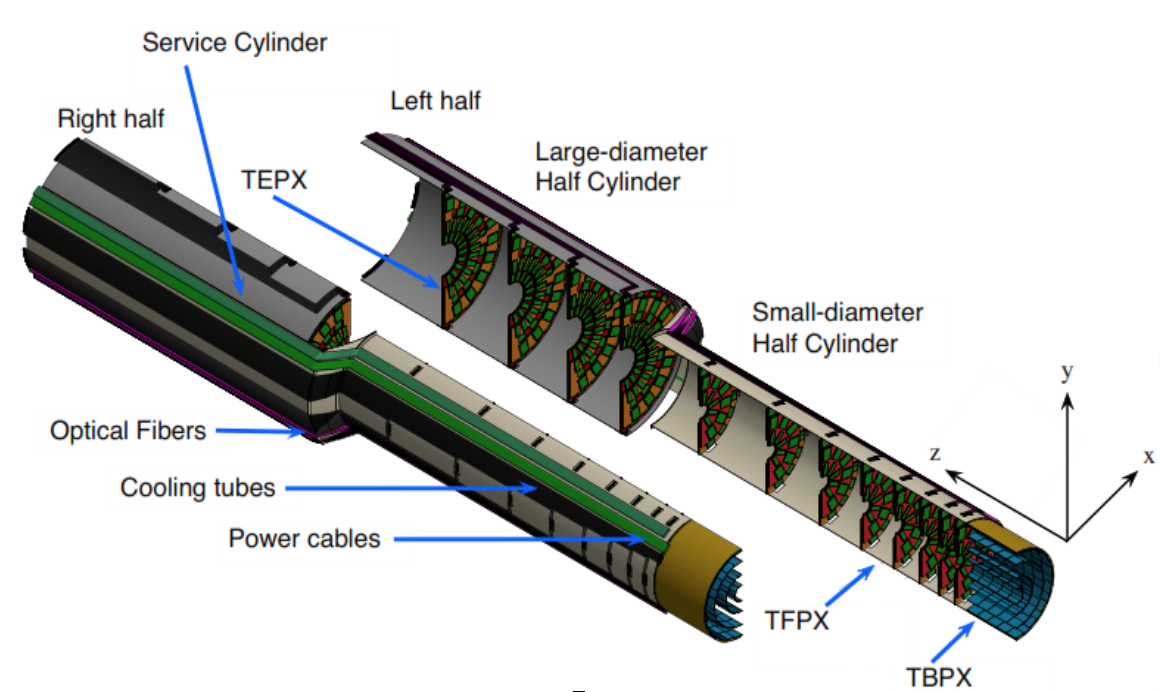
\includegraphics[width=0.8\textwidth]{PixelDet.png} 
\caption{Phase-2 Pixel Detector Layout[ref].}
\label{PixelDet} 
\end{center}
\end{figure}

The Phase-2 Pixel Detector\cite{Phase2Tracker,Phase2Tracker2} baseline design comprises a barrel part with 4 layers of Tracker Barrel Pixel Detector (TBPX), 8 small double-discs per side of Tracker Forward Pixel Detector (TFPX) and 4 large double-discs per side of Tracker Endcap Pixel Detector (TEPX). This forward and end part is referred to as 8l4s (8 TFPX and 4 TEPX). In the TBPX the pixel modules are arranged in ``ladders''. In each layer, neighboring ladders are mounted staggered in radius, so that $r$-$\phi$ overlap between the ladders is achieved. The modules on a ladder do not overlap in $z$. A projective gap at $\eta = 0$ is avoided by mounting an odd number of modules along $z$, and by splitting the barrel mechanics in $z$ into slightly asymmetric halves. In TFPX and TEPX the modules are arranged in concentric rings. Each double-disc is physically made of two discs, which facilitates to mount modules onto four planes, with overlaps in $r$ as well as $r$-$\phi$. Each disc is split into two halves, and these D-shaped structures are referred to as ``dees''. The TEPX will provide the required luminosity measurement capability, by an appropriate implementation of the readout architecture. In total, the pixel detector will have an active surface of approximately 4.9 m$^2$. \autoref{PixelDet} shows the layout of the Phase-2 Pixel Detector.







\chapter{What is Machine Learning?\label{ML}}
\section{Introduction}

An overview of a search for Supersymmetry in the all-hadronic channel with missing transverse momentum and a customized top tagger is presented. The data used for the analysis was collected in 2016 by the CMS experiment at the LHC, and corresponds to an integrated luminosity of 35.9 fb$^{-1}$ from proton-proton collisions at a center-of-mass energy ($\sqrt{s}$) of 13 TeV. The results and procedures presented are the product of an analysis conducted in collaboration with the hadronic SUSY analysis team based at Fermilab in Batavia, IL, USA. The published results can be obtained from \cite{SUSYanalysis}.

\section{Analysis Description}

The study consists of an inclusive search for events with final states that contain missing transverse momentum ($p_{\text{T}}^{miss}$) and reconstructed top quarks. The signal models used in this study include the production of three different types of SUSY particles. Two of which are the top squark ($\tilde{t}$) and the gluino ($\tilde{g}$), the supersymmetric partners of the SM top quark (t) and gluon (g). The third one is the neutralino ($\tilde{\chi}_{1}^{0}$), considered to be the lightest SUSY particle (LSP) under the Minimal Supersymmetric Standard Model (MSSM), and a possible candidate for Dark Matter.\\

The signal data is selected by requiring events to have a minimum amount of jets ($N_\text{j}$) and b-jets ($N_\text{b}$) as well as a large $p_{\text{T}}^{miss}$. Other factors, such as the number of top jets ($N_\text{t}$), the scalar sum of the jet transverse momentum ($H_\text{T}$), and the so-called stransverse mass ($m_\text{T2}$)\footnote{$m_\text{T2}$ is a minimization of two transverse masses ($m_\text{T}$) with a constraint that the sum of the transverse momenta of both $\tilde{\chi}_{1}^{0}$'s is equal to the transverse momentum of the event, i.e., $\vec{p}_\text{T} = \vec{q}_\text{T}^{(1)} + \vec{q}_\text{T}^{(2)}$. The mathematical definition is given by $m_\text{T2} \equiv \underset{\vec{q}_\text{T}^{(1)} + \vec{q}_\text{T}^{(2)} = \vec{p}_\text{T}}{\text{min}}\left [ \text{max}\left \{ m_\text{T}^2 (\vec{p}_\text{T}^{(1)}, \vec{q}_\text{T}^{(1)}; m_{\tilde{\chi}_{1}^{0}}), (\vec{p}_\text{T}^{(2)}, \vec{q}_\text{T}^{(2)}; m_{\tilde{\chi}_{1}^{0}}) \right \} \right ]$.} are also considered in order to select events of interest. The search region is then defined in exclusive bins of $N_\text{t}$, $N_\text{b}$, $H_\text{T}$, $p_{\text{T}}^{miss}$ and $m_\text{T2}$. Additional discriminatory variables used in the analysis include the azimuthal angle between $p_{\text{T}}^{miss}$ and the leading jets of an event ($\Delta\phi$), the pseudorapidity ($\eta$) and the cone radius size (defined as $\Delta R = \sqrt{(\Delta\eta)^2+(\Delta\phi)^2}$) used in the isolation of various physics objects.

\subsection{Signal Models}

The signal models used in this analysis are based on two different scenarios: direct top squark production and gluino mediated top squark production. In the former scenario we consider one decay within the Simplified Model Spectra (SMS)\cite{SMS} framework called `T2tt' (\autoref{SignalModels.png}, top left), where a top squark pair is produced directly from the proton-proton collision and then decays into a pair of top quarks and a pair of neutralinos ($\tilde{\text{t}}\rightarrow\text{t}\tilde{\chi}_{1}^{0}$).\\

\begin{figure}[H]
\begin{center}
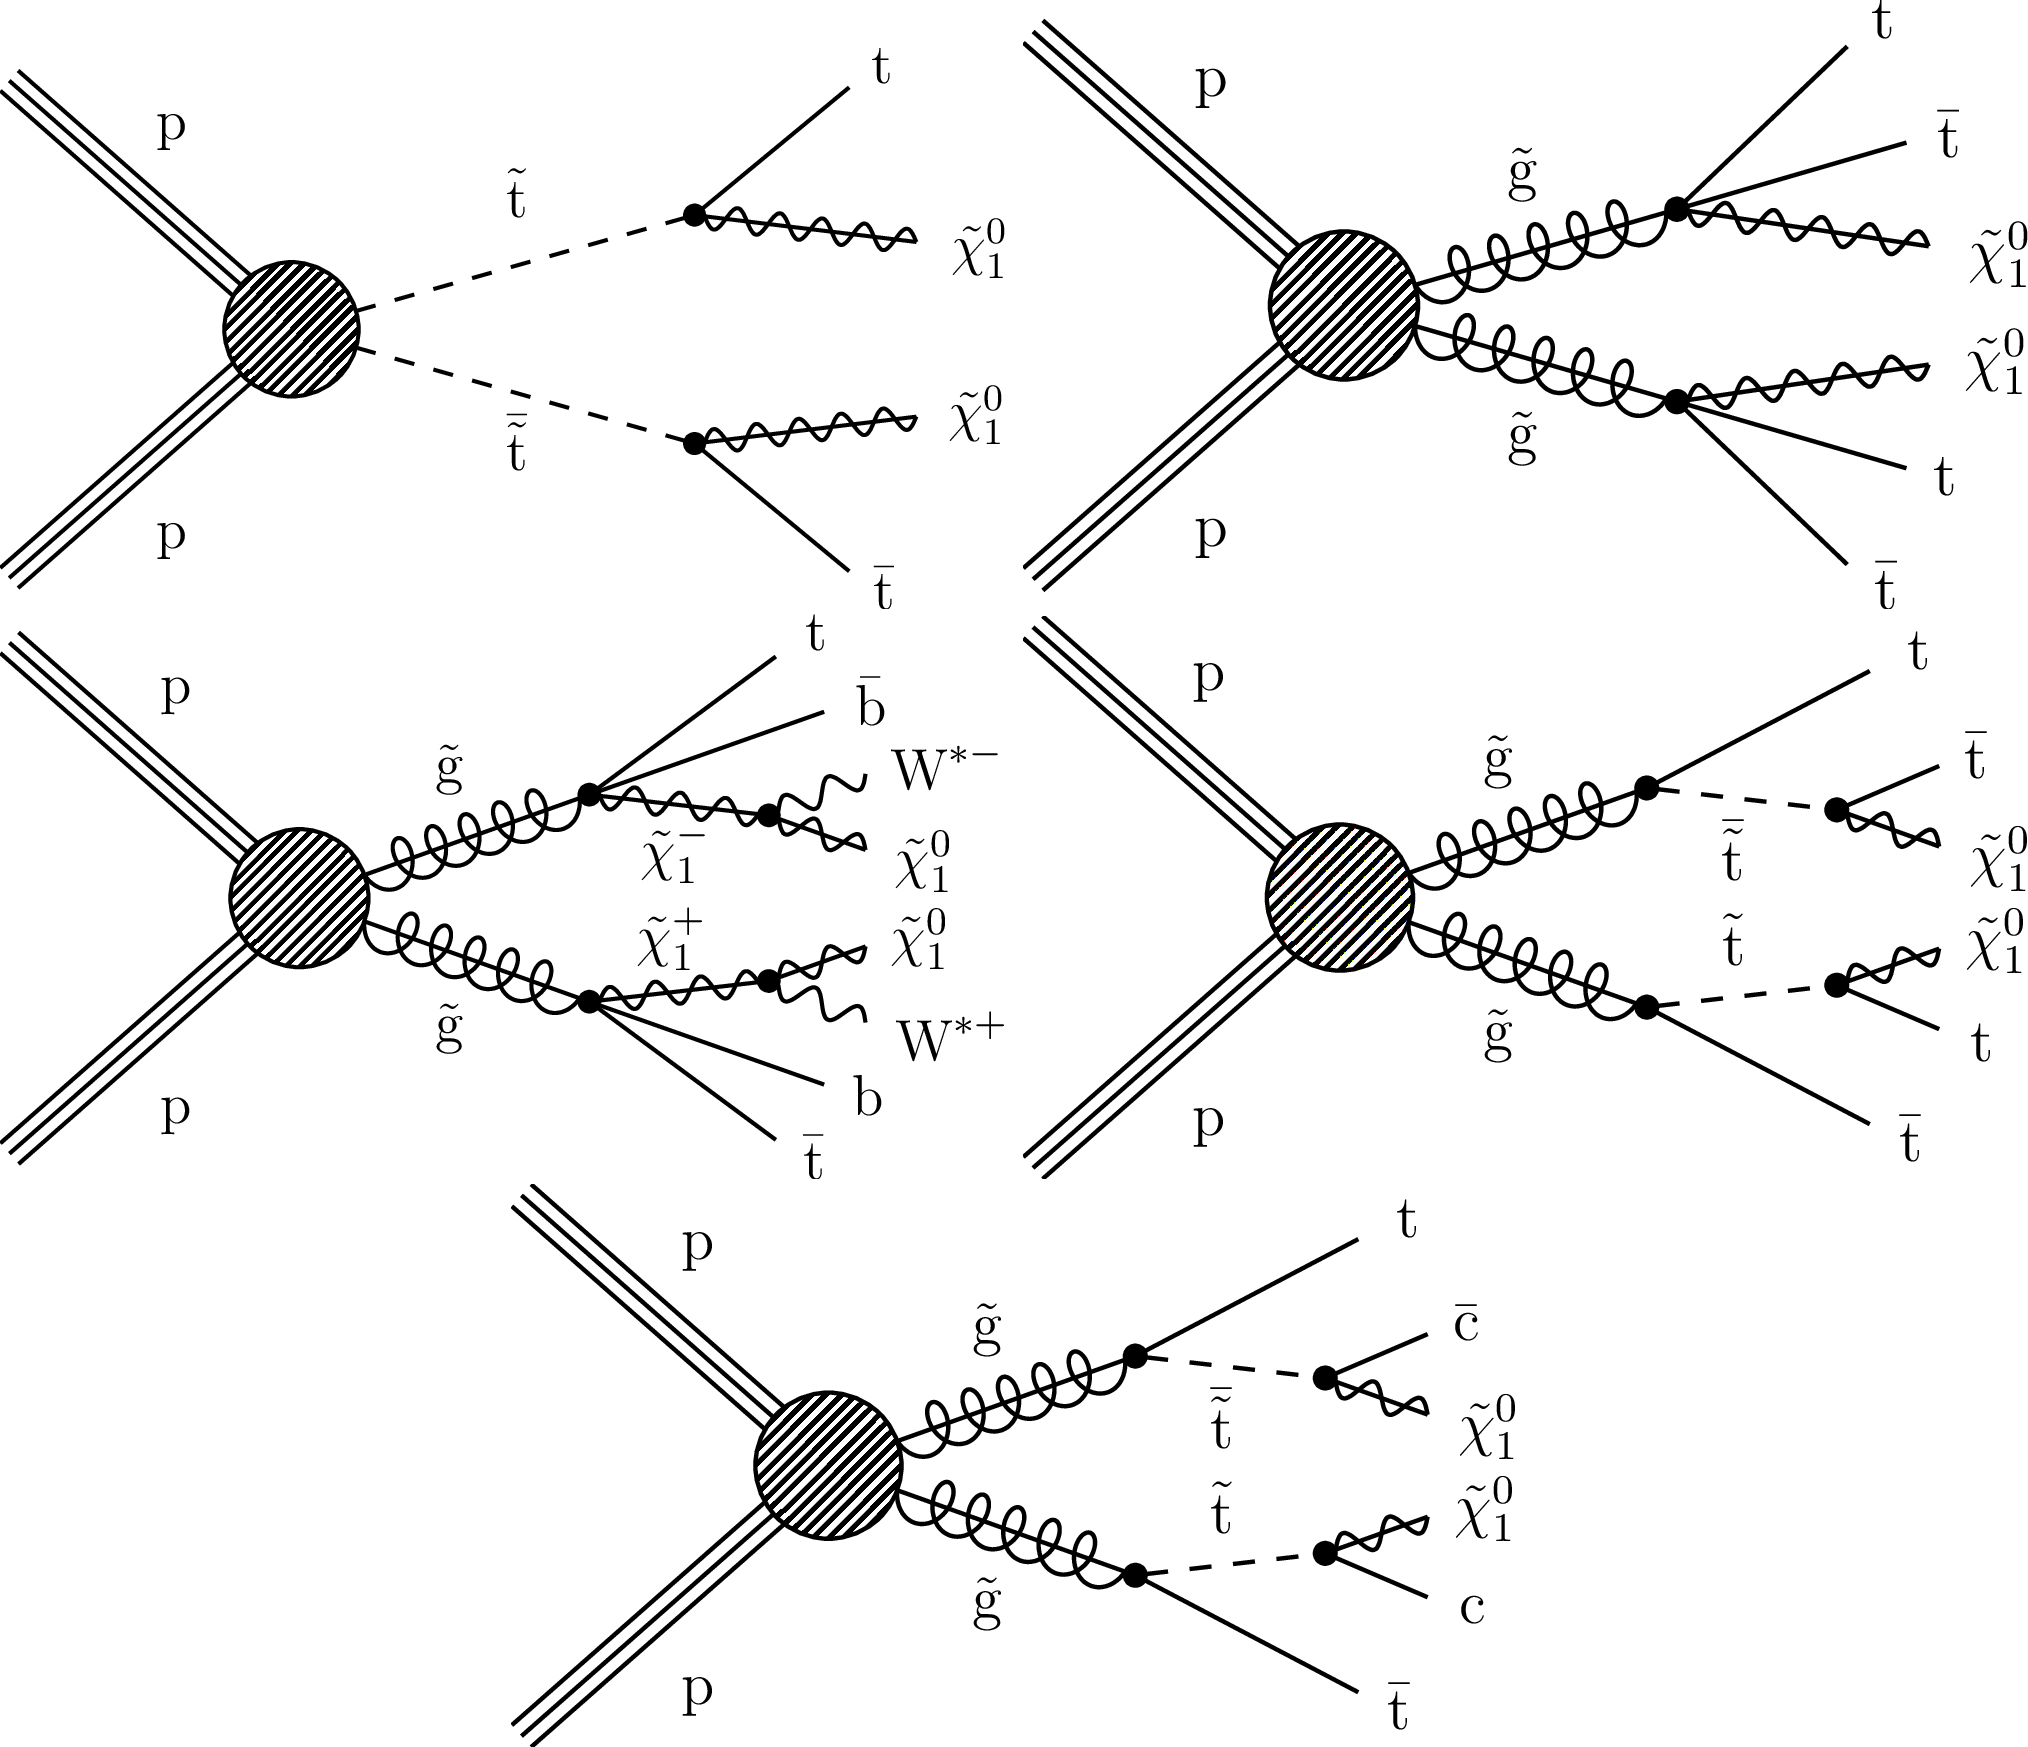
\includegraphics[width=0.92\textwidth]{SignalModels.png} 
\caption{Simplified model diagrams show of the various Supersymmetry signals considered in this analysis: the T2tt model (top left), the T1tttt model (top right), the T1ttbb model (middle left), the T5tttt (middle right), and the T5ttcc model (bottom).}
\label{SignalModels.png} 
%\hspace{4em}
\end{center}
\end{figure}

In the case of gluino mediated top squark production there are several different decay modes considered. The T1tttt model (\autoref{SignalModels.png}, top right) consists of two gluinos decaying into a pair of top quarks and a neutralino ($\tilde{\text{g}}\rightarrow\text{t}\bar{\text{t}}\tilde{\chi}_{1}^{0}$), accounting for situations in which the top squark is too heavy to be produced directly but the gluino is not. In the T1ttbb model (\autoref{SignalModels.png}, middle left), a pair of gluinos to either a top or bottom squark as $\tilde{\text{g}}\rightarrow\text{t}\bar{\text{t}}\tilde{\chi}_{1}^{0}$ (25\%), $\tilde{\text{g}}\rightarrow\text{b}\bar{\text{b}}\tilde{\chi}_{1}^{0}$ (25\%), or $\tilde{\text{g}}\rightarrow\bar{\text{t}}\text{b}\tilde{\chi}_{1}^{\pm}$ (50\%), where $\tilde{\chi}_{1}^{\pm}$ denotes the lightest positive ($\tilde{\chi}_{1}^{+}$) or negative ($\tilde{\chi}_{1}^{-}$) chargino. Due to the small difference in mass between the $\tilde{\chi}_{1}^{+}$ (or its conjugate) and the LSP ($\Delta m(\tilde{\chi}_{1}^{+},\tilde{\chi}_{1}^{0}) = 5$ GeV), the two particles are taken to be nearly mass degenerate. The T1ttbb model provides sensitivity to situations where there are mixed states of top and bottom squarks.\\

The T5tttt model consists of a pair of gluinos, where each decays into a top quark and an on-shell top squark. The top squark then decays into a top quark and a neutralino. For this model, a mass difference of $\Delta m(\tilde{\text{t}},\tilde{\chi}_{1}^{0}) = 175$ GeV between the top squark and the LSP is expected. This model provides sensitivity to a region of T2tt where the t$\bar{\text{t}}$ background is very similar to the signal and $\Delta m(\tilde{\text{t}},\tilde{\chi}_{1}^{0})$ is very close to the top squark mass. In the T5ttcc model (\autoref{SignalModels.png}, bottom) each gluino decays into a final state consisting of a top quark, a charm quark and a neutralino ($\tilde{\text{g}}\rightarrow\bar{\text{t}}\text{c}\tilde{\chi}_{1}^{0}$). This model is very similar to the T5tttt model with the difference that $\Delta m(\tilde{\text{t}},\tilde{\chi}_{1}^{0}) = 20$ GeV and the on-shell top squark decays into a charm quark and the LSP. The T5ttcc model provides sensitivity to situations where the on-shell top squark is kinematically forbidden from decaying into a top quark.\\

All five signal models described share similar final states containing two neutralinos and up to four top quarks. Since the neutralino is considered stable and only interacts weakly with matter, it cannot be picked up by the detector. Therefore, missing transverse momentum ($p_{T}^{miss}$) is one of the most important variables used to compare event yields between the signal and the SM background.

\subsection{Top Tagger}\label{TopTaggerSec}

The distinguishing feature of this analysis is its powerful top-tagging algorithm. It is designed to provide high reconstruction efficiency over the full range of the top quark $p_\text{T}$ for the considered SUSY signal models. This top-tagger combines the use of several different jet clustering algorithms in order to identify three different categories of top quark jets, designated as ``monojet'', ``dijet'' and ``trijet''. The tagger makes use of identified jets that were reconstructed with the anti-$k_\text{T}$\cite{AntiKt} clustering algorithms combined with additional corrections and selection criteria provided by the Cambridge--Aachen\cite{JetAlg1} and soft-drop de-clustering\cite{SoftDrop} algorithms. In addition, multivariate analysis (MVA) techniques, such as the random forest decision tree algorithm\cite{RandForest1}, were applied in order to further decrease the amount of reconstructed fake tops.\\

There are three top-quark jet categories that take into account that top quark decay products get closer together as the top quark $p_\text{T}$ becomes higher. For specific $p_\text{T}$ values, the decay products of a hadronic process will be reconstructed either as one (``monojet'') or two (``dijet'') jets rather than three (``trijet''). The $p_\text{T}$ values for which this is observed depends on the size of the jets that are being used. In the case of a highly boosted jet, the anti-$k_\text{T}$ algorithm is used within a cone size $\Delta R \sim 0.8$ (called AK8), which captures all decay products of the top quark and is reconstructed as a single jet. This technique requires that the top quark starts with a $p_\text{T}$ of at least 400 GeV to have the decay products fully captured in the 0.8 jet cone. For a $p_\text{T} < 400$ GeV, resolved top-tagging techniques are more efficient, which require three jets independently clustered within a cone size of $\Delta R \sim 0.4$ (AK4). Both types of algorithms are used in order to obtain a high efficiency over a wide range of top quark $p_\text{T}$.

\begin{figure}[H]
\begin{center}
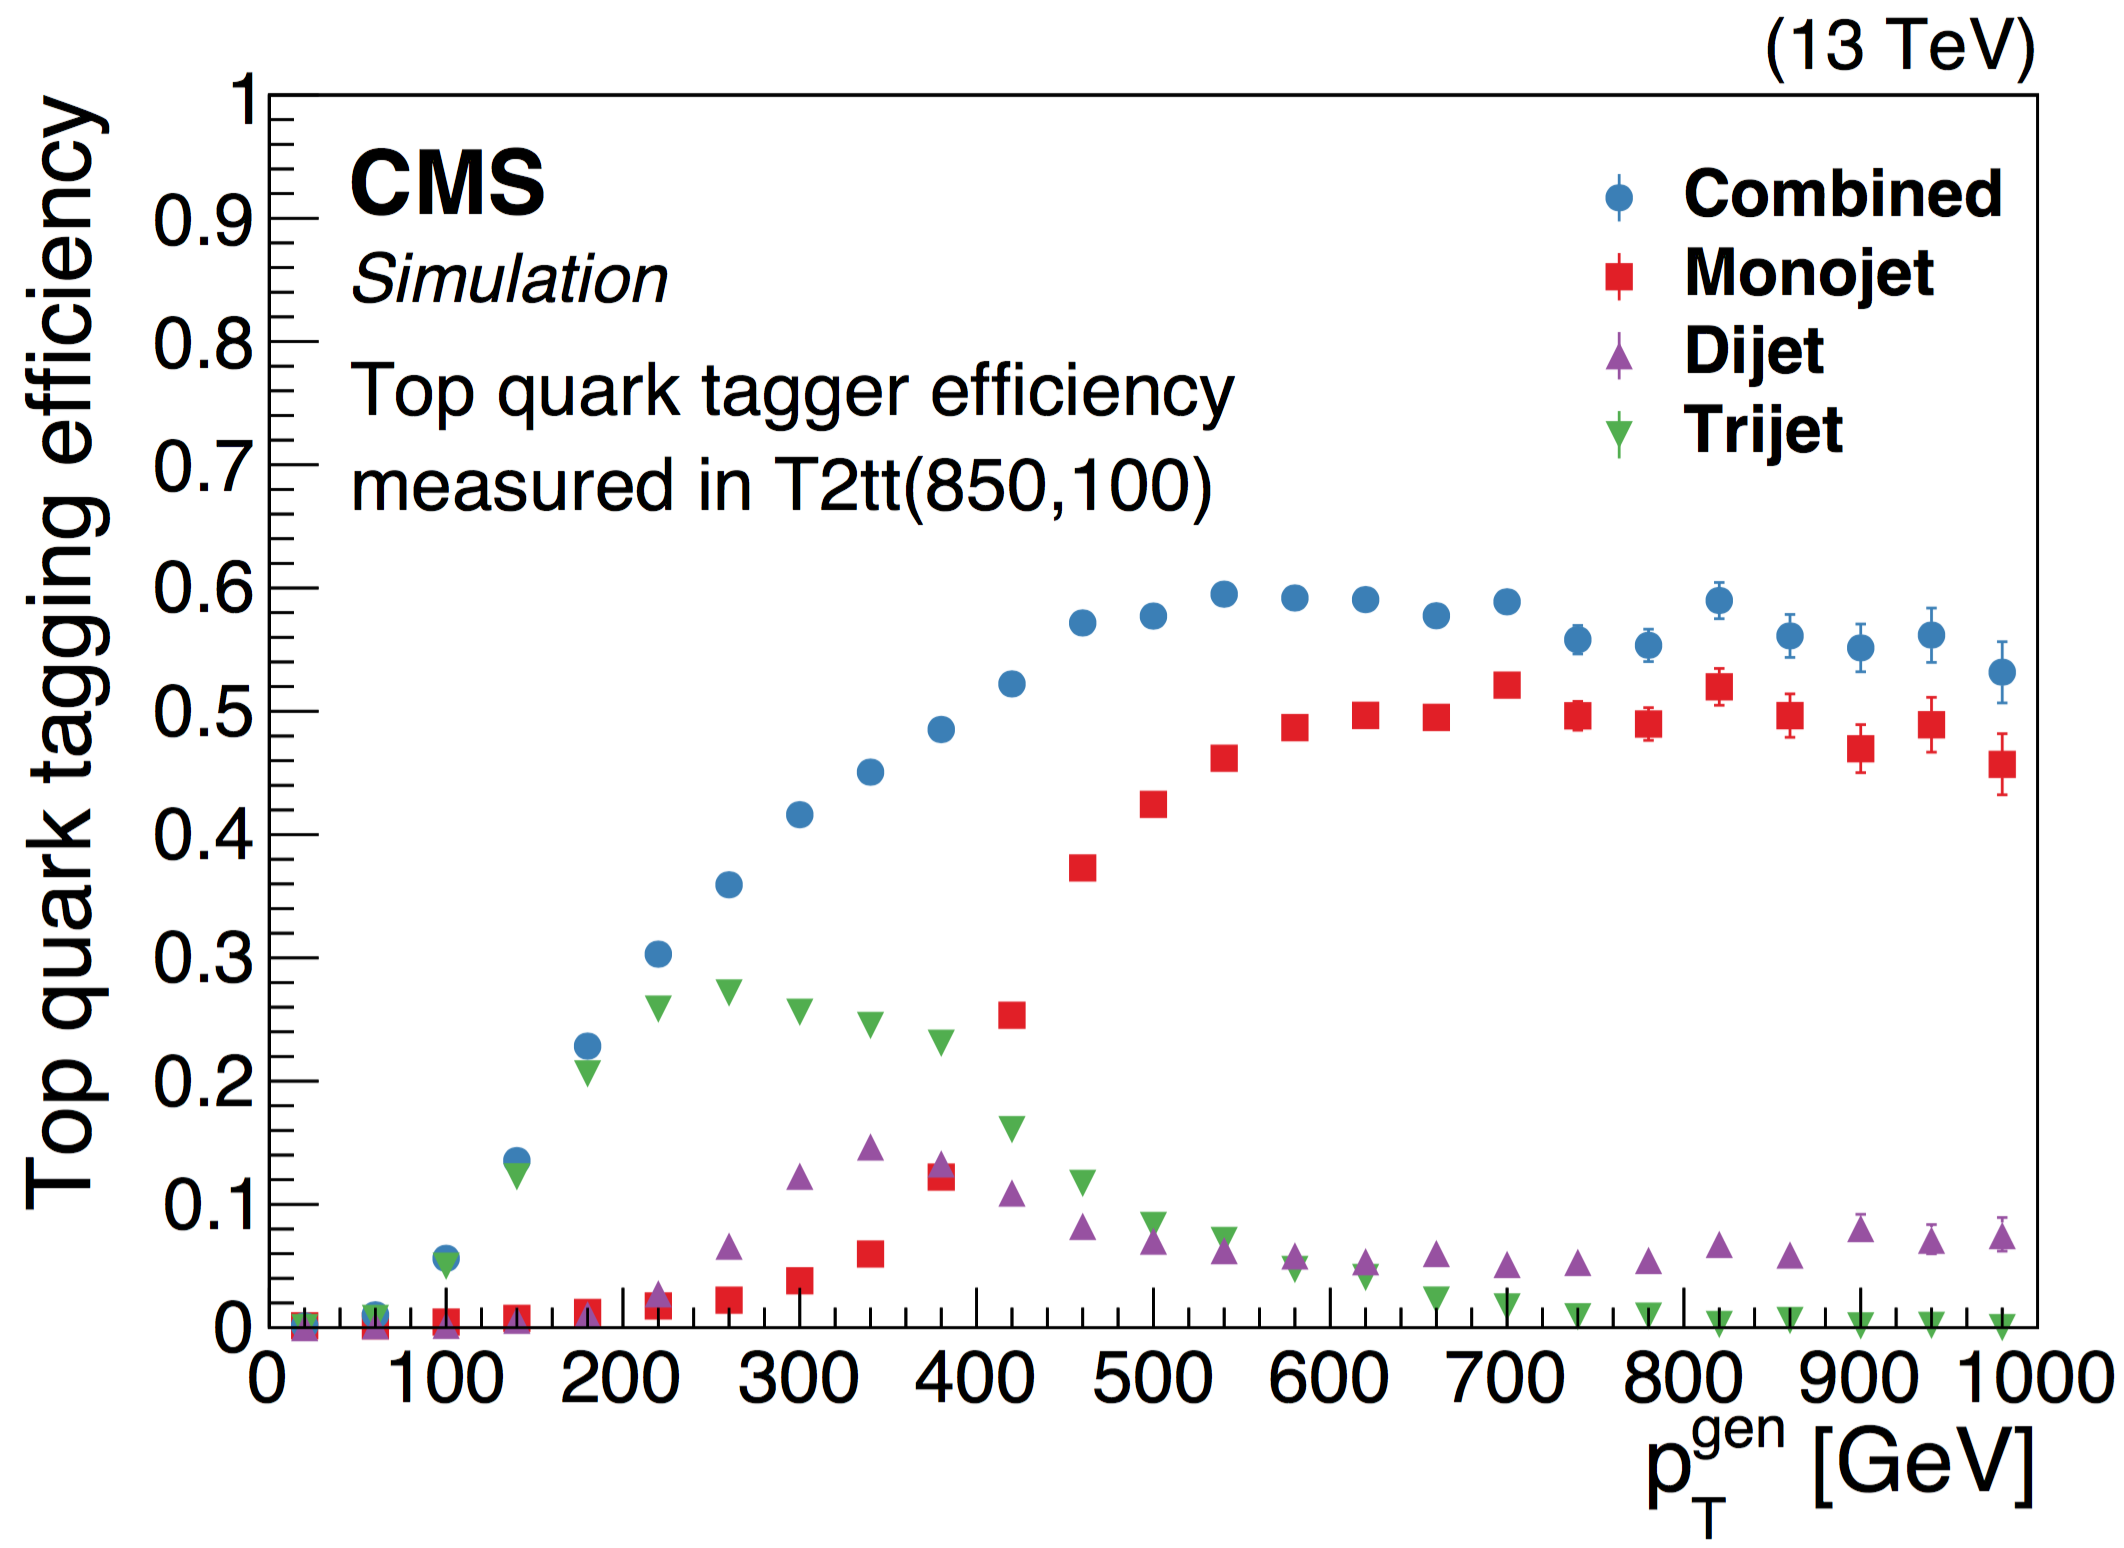
\includegraphics[width=0.8\textwidth]{TopTaggerEff.png} 
\caption{Efficiency of the top quark tagger as a function of generator-level top quark $p_\text{T}$ for the monojet (red boxes), dijet (magenta triangles), and trijet (green upside-down triangles) categories and for their combination (blue circles), as determined using T2tt signal events with a top squark mass of 850 GeV and an LSP mass of 100 GeV. The vertical bars indicate the statistical uncertainties.}
\label{TopTaggerEff} 
\end{center}
\end{figure}

In the case of the dijet top quark decay category, an AK8 jet with a $p_\text{T} > 200$ GeV is combined with a loose AK4 jet to form a top quark candidate. Both jets are required to be within a cone of radius $\Delta R = 1$. For the trijet category, three AK4 jets are combined, with all three jets required to be within a radius of $\Delta R = 1.5$. \autoref{TopTaggerEff} shows the efficiency of the algorithm for each of the three categories of top jets. The efficiency was determined for the T2tt signal model considering a top squark mass of 850 GeV and an LSP mass of 100 GeV, and is calculated as:
\begin{center}
Efficiency $= \dfrac{\text{Number of generator-level top quarks matched to a tagged top}}{\text{Number of generator-level top quarks in an event}}$.
\end{center}

The top quark candidates are required to be within $|\eta| < 2.0$. Furthermore, a cone size of $\Delta R < 0.4$ is used to match the reconstructed top quark to the generated-level top quark. The average misidentification rate as a function of the $p_\text{T}^{miss}$ is found to be around 20\% for simulated Z($\nu\bar{\nu}$)+jets events with a selection criteria similar to the one applied to data: $N_j \geq 4$, $N_b \geq 1$, $p_\text{T}^{miss} > 250$ GeV and no isolated electron or muon with $p_\text{T} > 10$ GeV.


\subsection{Lepton and Track Vetoes}\label{lepVeto}

Since the search only involves models with purely hadronic final states, events which contain electrons or muons are vetoed. This requires the isolation of the muon/electron candidates to a cone size of $\Delta R < 0.2$ for $p_\text{T} \leq 50$ GeV and 0.05 for $\geq 200$ GeV. This $\Delta R$ requirement decreases inversely to the lepton $p_\text{T}$ in the range $50 < p_\text{T} < 200$ GeV in order to account for the collimation of a heavy object's decay products as its Lorentz boost increases. The electron and muon objects are considered to be isolated when their relative isolation\footnote{The ratio between the isolation sum and the candidate $p_\text{T}$.} is less than 0.1 and 0.2, respectively. Due to contributions from pileup, the isolation sum is corrected using an estimate of the amount of pileup energy in the cone.\\

The events that manage to pass the lepton veto are subjected to undergo an isolated charged-particle track veto. The purpose of this veto is to suppress events which contain $\tau$ leptons that decay hadronically or misidentified electrons and muons. The track requirements for this veto are $p_\text{T} > 5$ GeV, $|\eta| < 2.5$ and a relative track isolation less than 0.2. In addition, the isolated track veto is only applied when the transverse mass of an isolated track-$\vec{p}_\text{T}^{miss}$ is $m_\text{T} < 100$ GeV, consistent with W boson decays. This veto successfully reduces the background of leptonically decaying W bosons by about 40\%.

\subsection{Baseline Event Selection}\label{baseline}

The data selection process begins with the triggers and follows with a pre-selection and the definition of the search bins. The selection criteria applied is optimized for high trigger efficiency as well as being sensitive to a variety of new-physics scenarios. The events selected from data meet the following baseline conditions:\\
 
\begin{itemize}
	\item{Satisfy the filters designed to remove detector and beam-related noise.}
	\item{Undergo the lepton, isolated-track, and charged-hadron vetoes.}
	\item{Have a final state with $N_\text{j} \geq 4$, $N_\text{b} \geq 1$, $N_\text{t} \geq 1$, $p_{\text{T}}^{miss} > 250$ GeV and $H_\text{T} > 300$ GeV.}
	\item{$m_\text{T2} > 200$ GeV, in order to reduce background contributions from t$\bar{\text{t}}$ events.}
	\item{To reduce the background arising from the QCD multijet background the azimuthal angle between the $p_{\text{T}}^{miss}$ and the three leading jets of an event is required to be $\Delta\phi(p_{\text{T}}^{miss},j_{1,2,3}) > 0.5, 0.5, 0.3$, where $j_1$, $j_2$, and $j_3$ indicate the three leading jets in order of decreasing $p_\text{T}$.}
\end{itemize}

\subsection{Search Bin Definition}\label{SearchBinDef}

The search described in this chapter was performed by defining 84 non-overlapping search regions (\autoref{SearchBins.png}). Regions that contain events with $N_\text{b} \leq 2$ and $N_\text{t} \leq 2$ use  $N_\text{b}$, $N_\text{t}$, $p_{\text{T}}^{miss}$ and $m_\text{T2}$. In contrast, if the events contain $N_\text{b} \geq 3$ and $N_\text{t} \geq 3$, then $N_\text{b}$, $N_\text{t}$, $p_{\text{T}}^{miss}$ and $H_\text{T}$ are used for that region. The reason $H_\text{T}$ is used for these regions instead of $m_\text{T2}$ has to do with the fact that for events that contain many jets, the jets arising from the decay of specially heavy objects are not always correctly associated with said object, giving the $m_\text{T2}$ variable a relatively broad and flat distribution. Therefore, in regions with $N_\text{b} \geq 3$ and $N_\text{t} \geq 3$, $H_\text{T}$ is found to provide better discrimination between signal and background.

\begin{figure}[tb]
\begin{center}
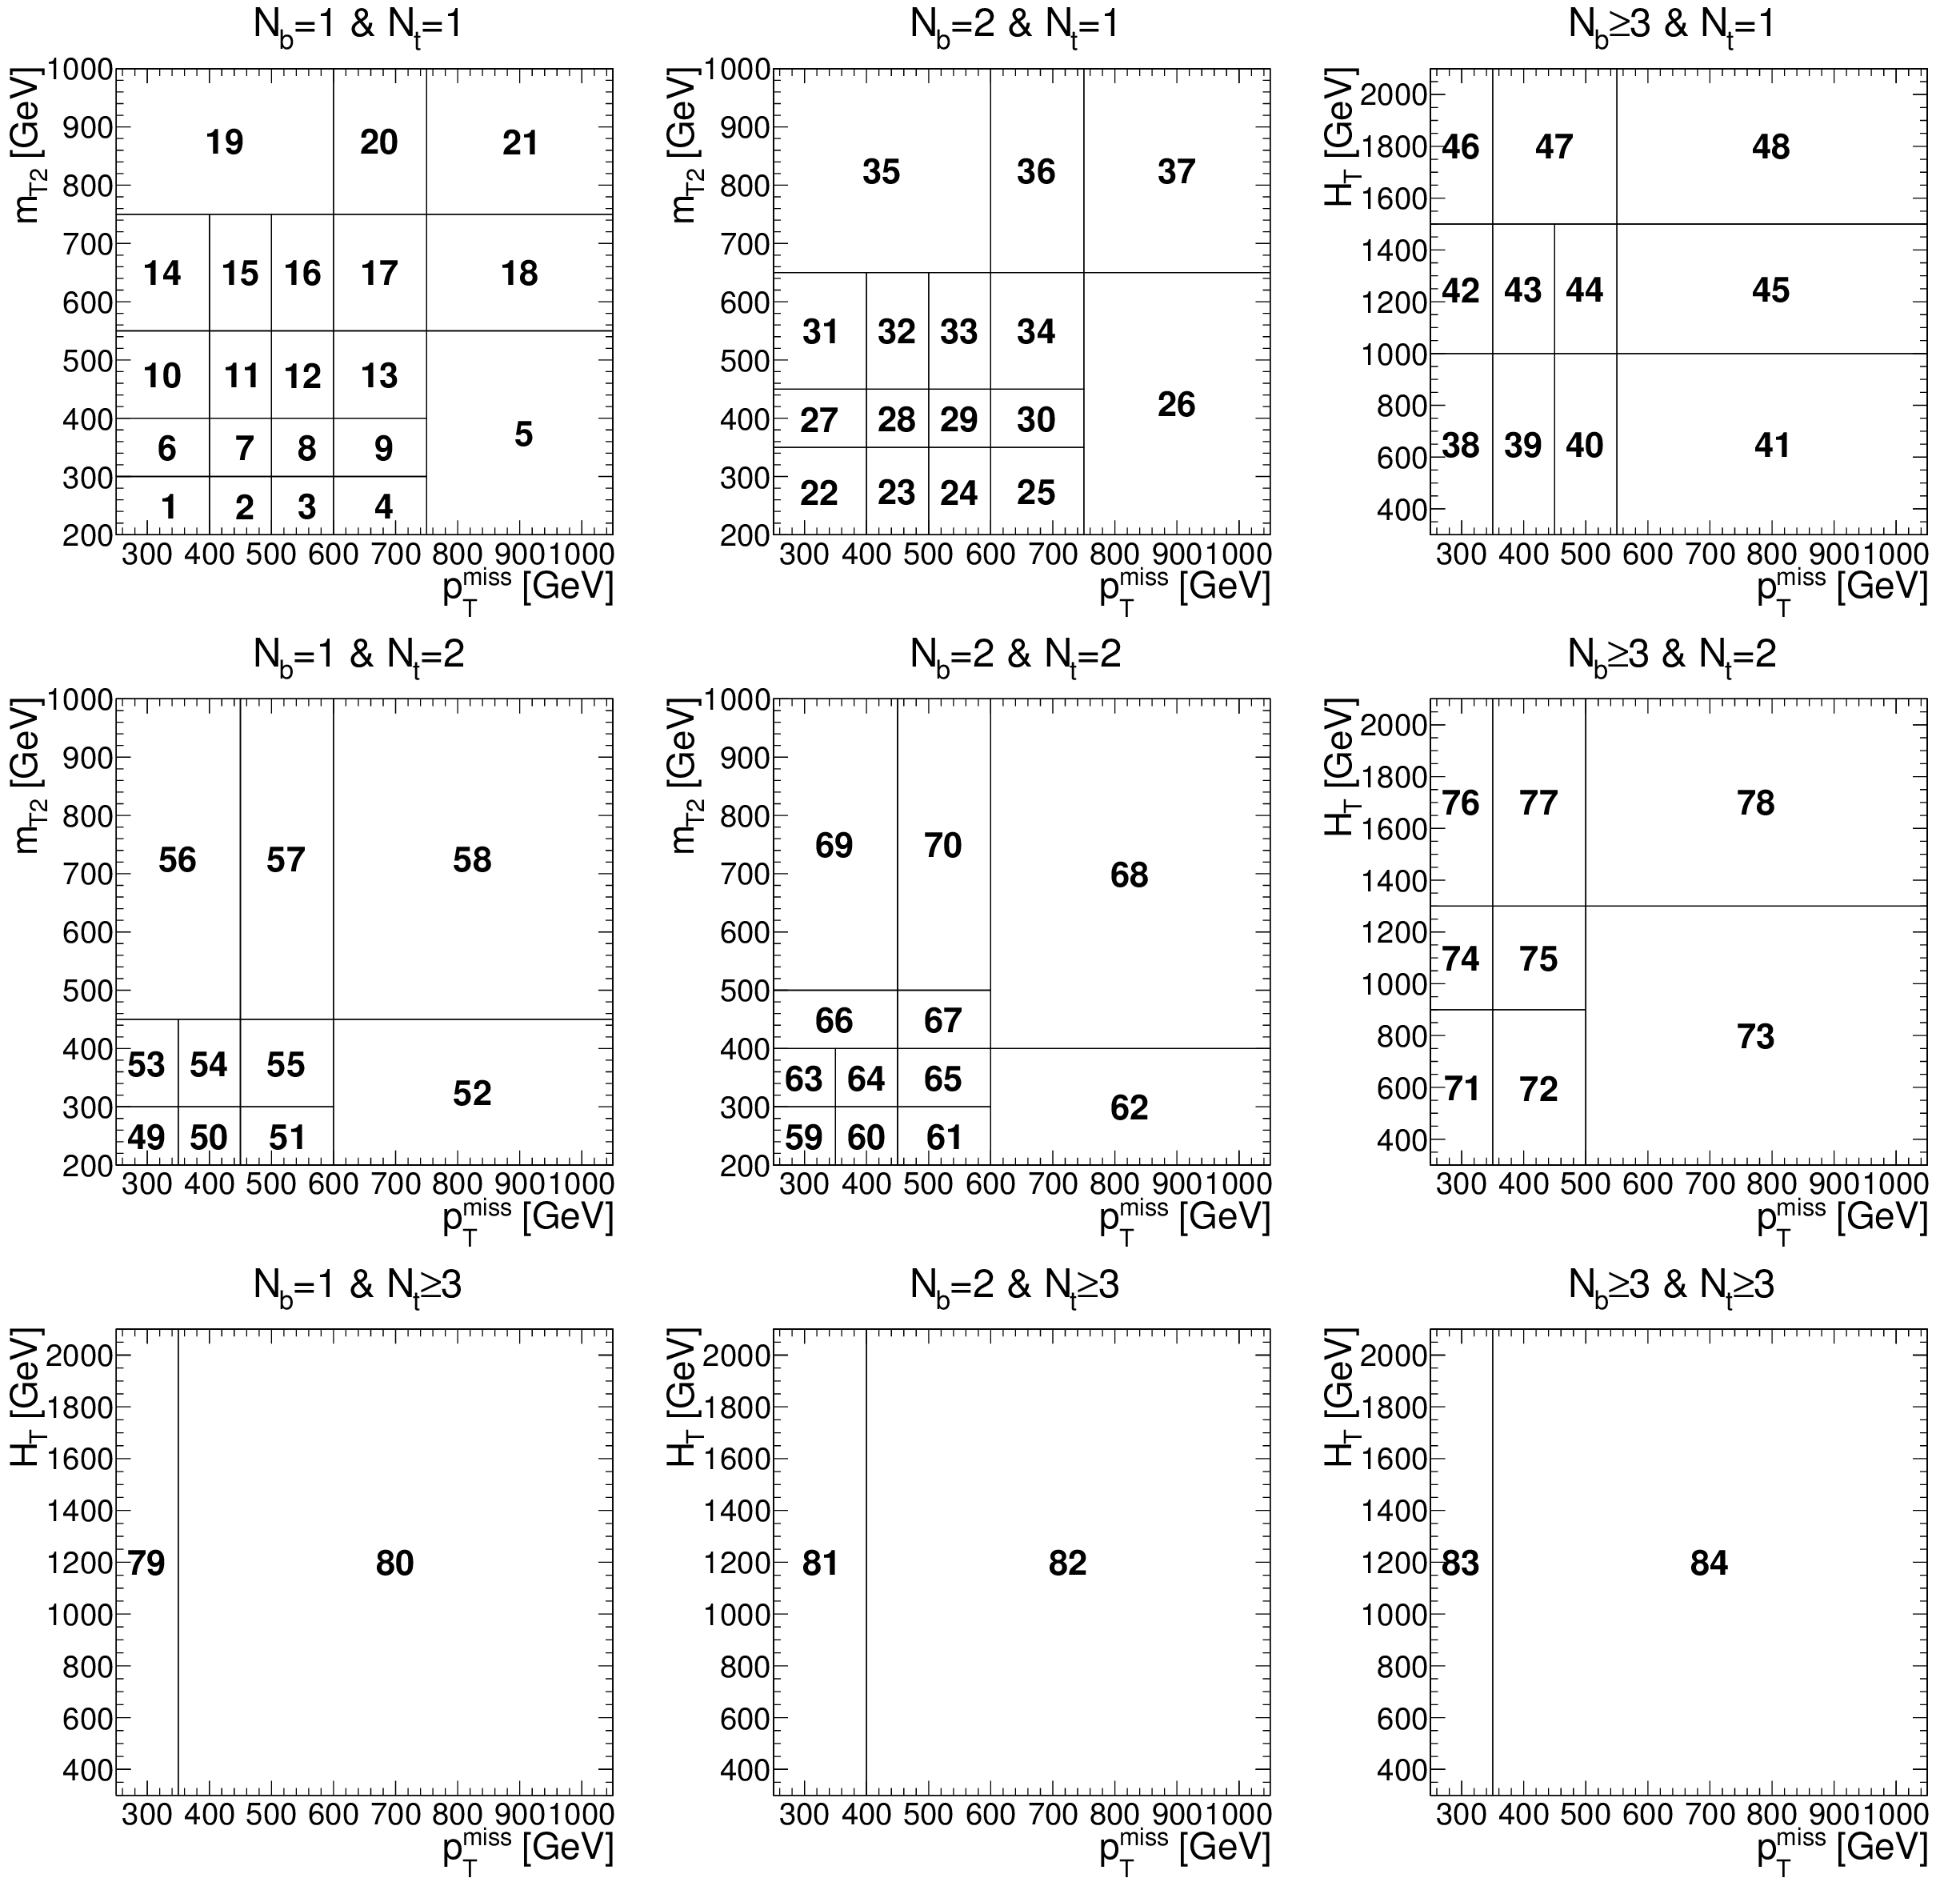
\includegraphics[width=0.9\textwidth]{SearchBins.png} 
\caption{Search region definitions in the kinematic variables.}
\label{SearchBins.png} 
\end{center}
\end{figure}

\section{Background Estimation}\label{backgrounds}

Since there are many SM processes which exhibit the same characteristics as those of the signal models (e.g. multiple jets, missing energy, etc.) it is of the utmost importance to be able to properly account for their contributions. These interactions, which closely resemble the signal that's being searched for, are called the SM background. However, they cannot be determined solely from the detector's reconstructed data itself, which is why MC simulation is used to recreate them using theoretical predictions from the SM. These simulations give us a good idea of what the signal region should look like if there were no signal events, and therefore any significant excess when comparing the MC background to data could signify a potential discovery. The relevant backgrounds for this particular analysis are: the lost-lepton background, the hadronic $\tau$ background, the Z $\rightarrow\nu \bar{\nu}$ background and the QCD multijet background.

\begin{figure}[tb]
\begin{center}
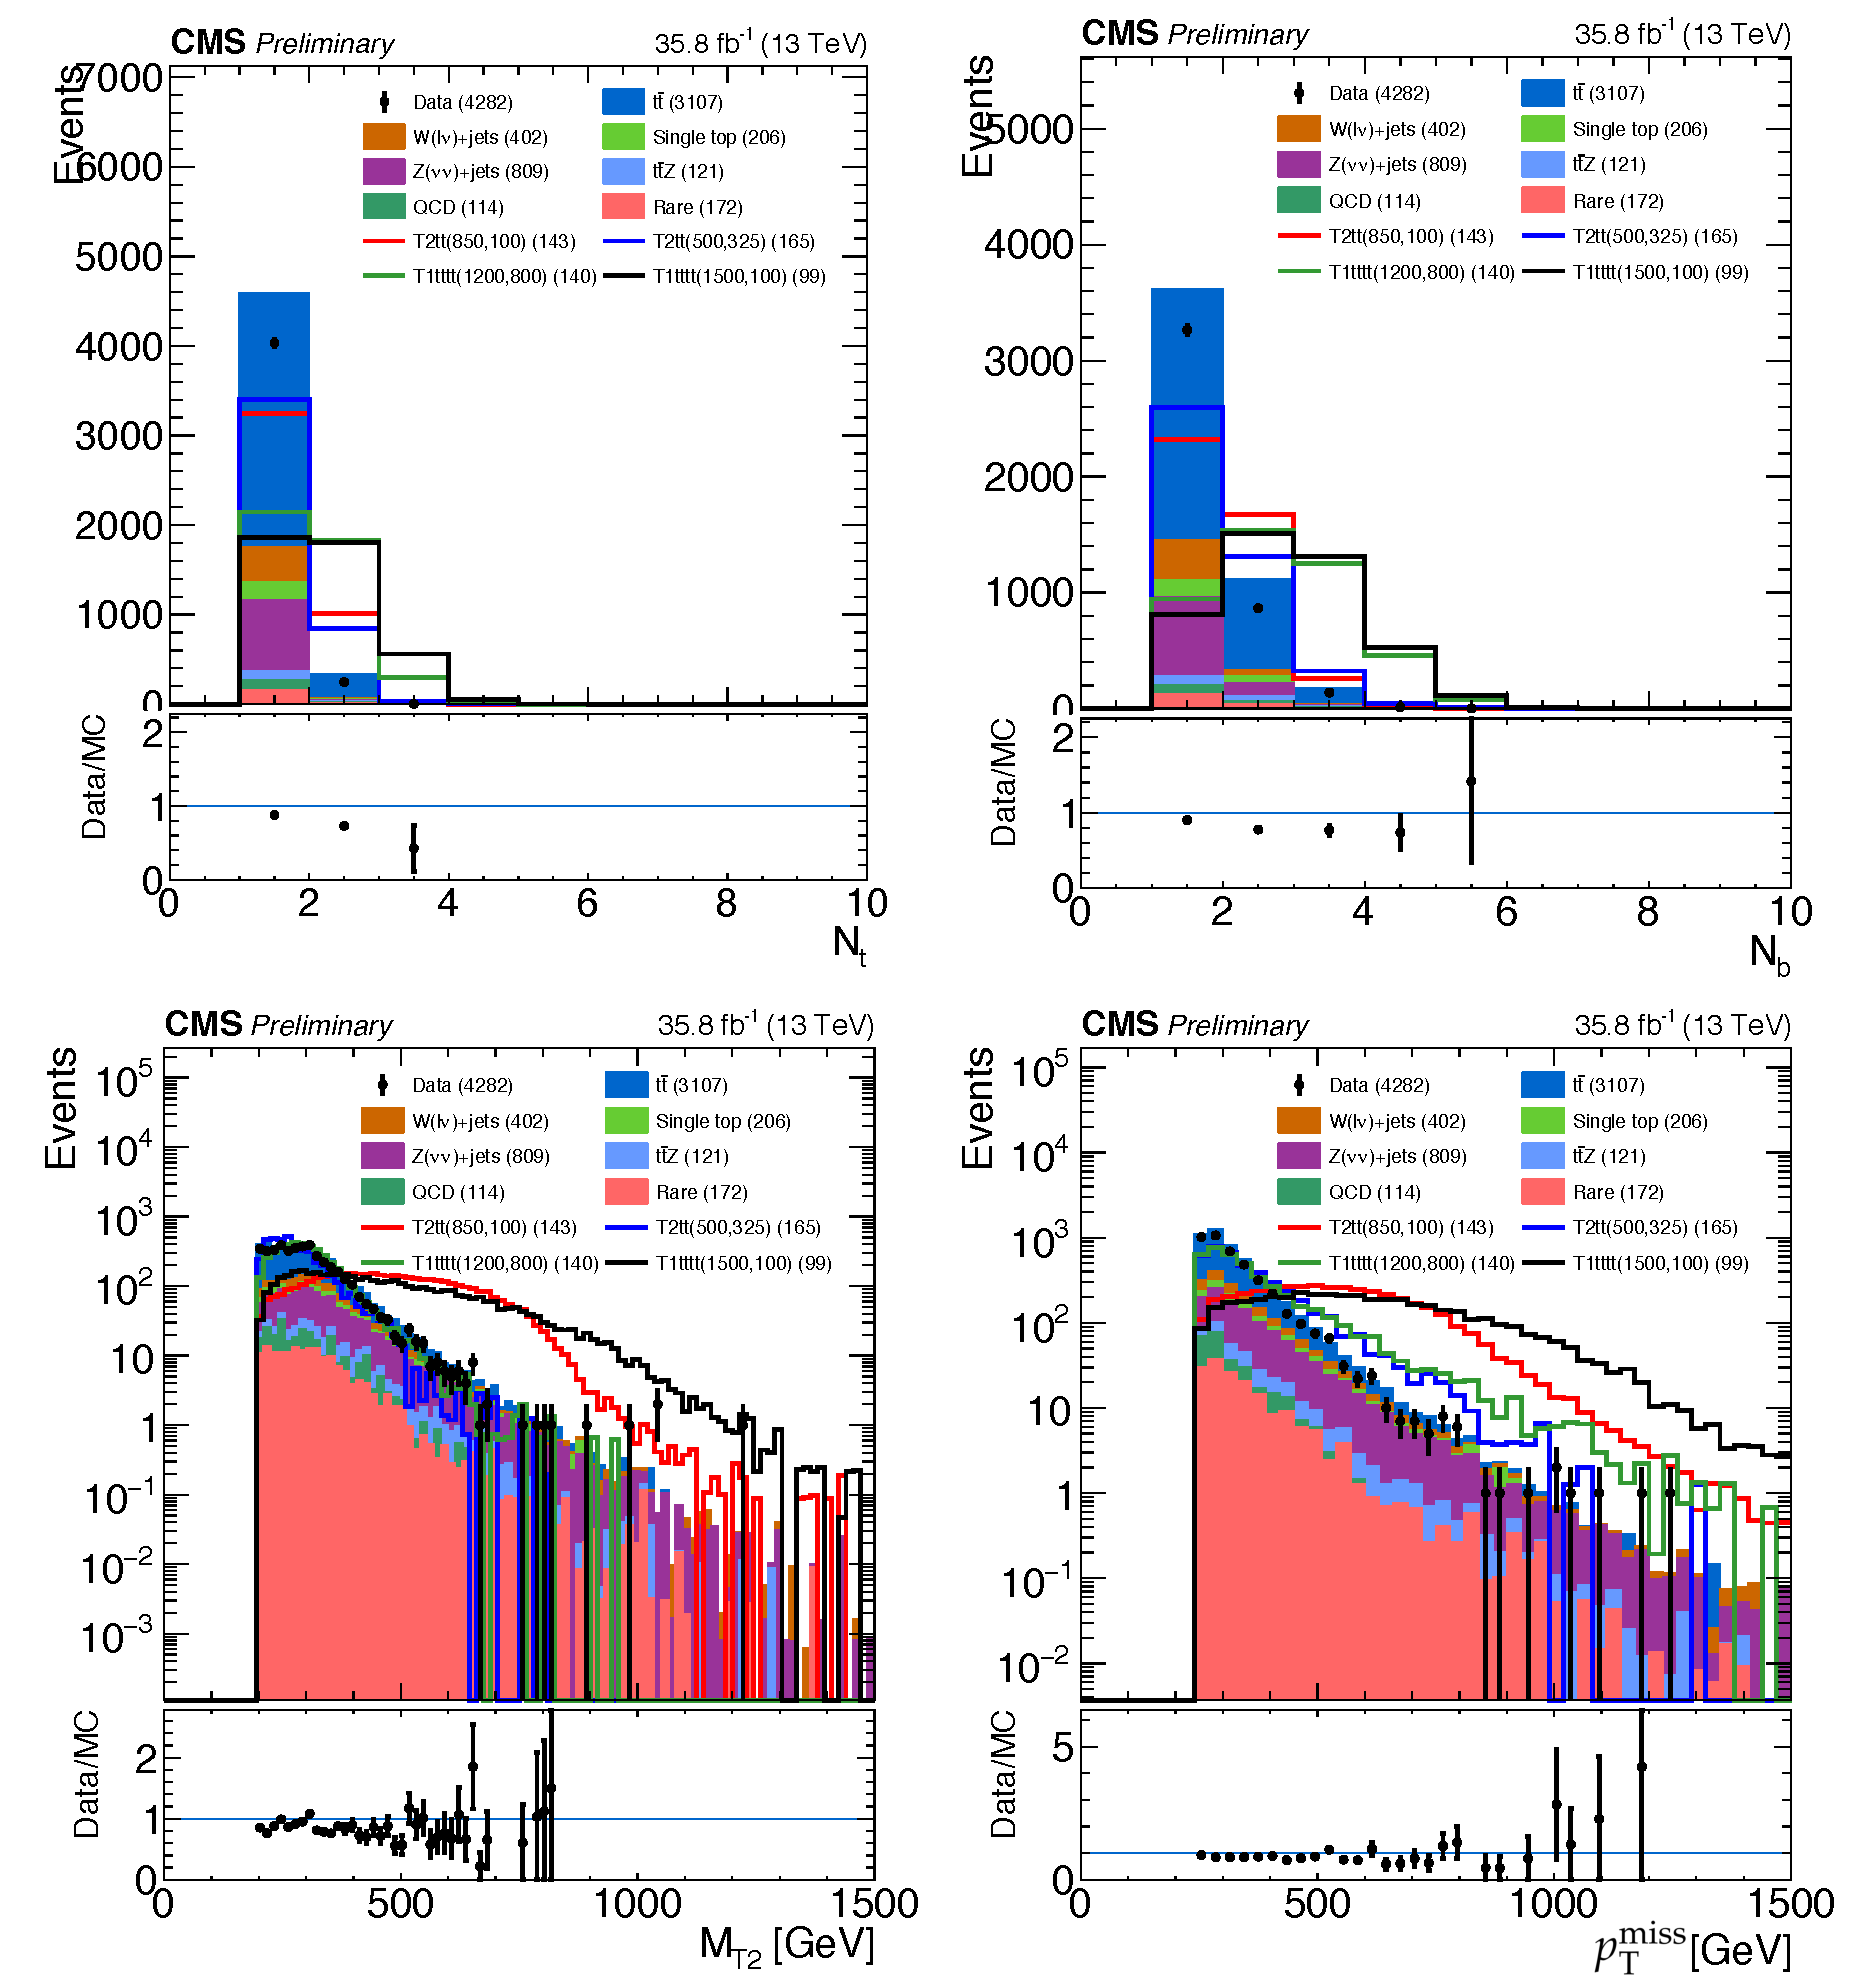
\includegraphics[width=0.9\textwidth]{MyPlots.pdf} 
\caption{Comparison between the total SM background from simulation and CMS data for $N_\text{t}$ (top left), $N_\text{b}$ (top right),  $m_\text{T2}$ (bottom left) and $p_{\text{T}}^{miss}$ (bottom right). Total SM backgrounds and signals are scaled to same data yield for a shape comparison.}
\label{MyPlots.pdf} 
\end{center}
\end{figure}

\subsection{Background from t$\bar{\text{t}}$, Single Top Quark and W+jets Events}

The vast majority of the expected SM background (around 70\%) is due to t$\bar{\text{t}}$ and W+jets events where the W decays into a lepton and a neutrino. Since the expected signal is purely hadronic, a portion of the leptonic and semi-leptonic decays are vetoed and do not form part of the total SM background. However, there are two different scenarios in which the lepton vetoes can be satisfied. For instance, when the W decays into a $\tau$ which decays hadronically ($\tau_\text{h}$), the $\tau$ gets reconstructed as a jet and passes the veto. If, on the other hand, the W decays into an electron or a muon, the veto is satisfied when the corresponding lepton is said to be ``lost". In other words, the lepton veto fails to reject events when light leptons (electrons and muons) are not isolated, not identified/reconstructed, or are out of the acceptance region. Both scenarios are evaluated together with a single-lepton data control sample (CS), subjected to the same trigger used for signal events.\\

The total predicted amount of lost-lepton and $\tau_\text{h}$ events in any given search region is defined by the net sum of single-electron and single-muon events in the respective CS, corrected by a translation factor that is determined from simulation. Due to differences in how they are detected, the single-electron and single-muon samples are determined separately. The translation factor used to correct the search bins is defined as the ratio of simulated $\tau_\text{h}$ and lost-lepton events in the search region over the number of simulated single-electron or single-muon events in the corresponding CS region.

\begin{figure}[H]
	\begin{center}
		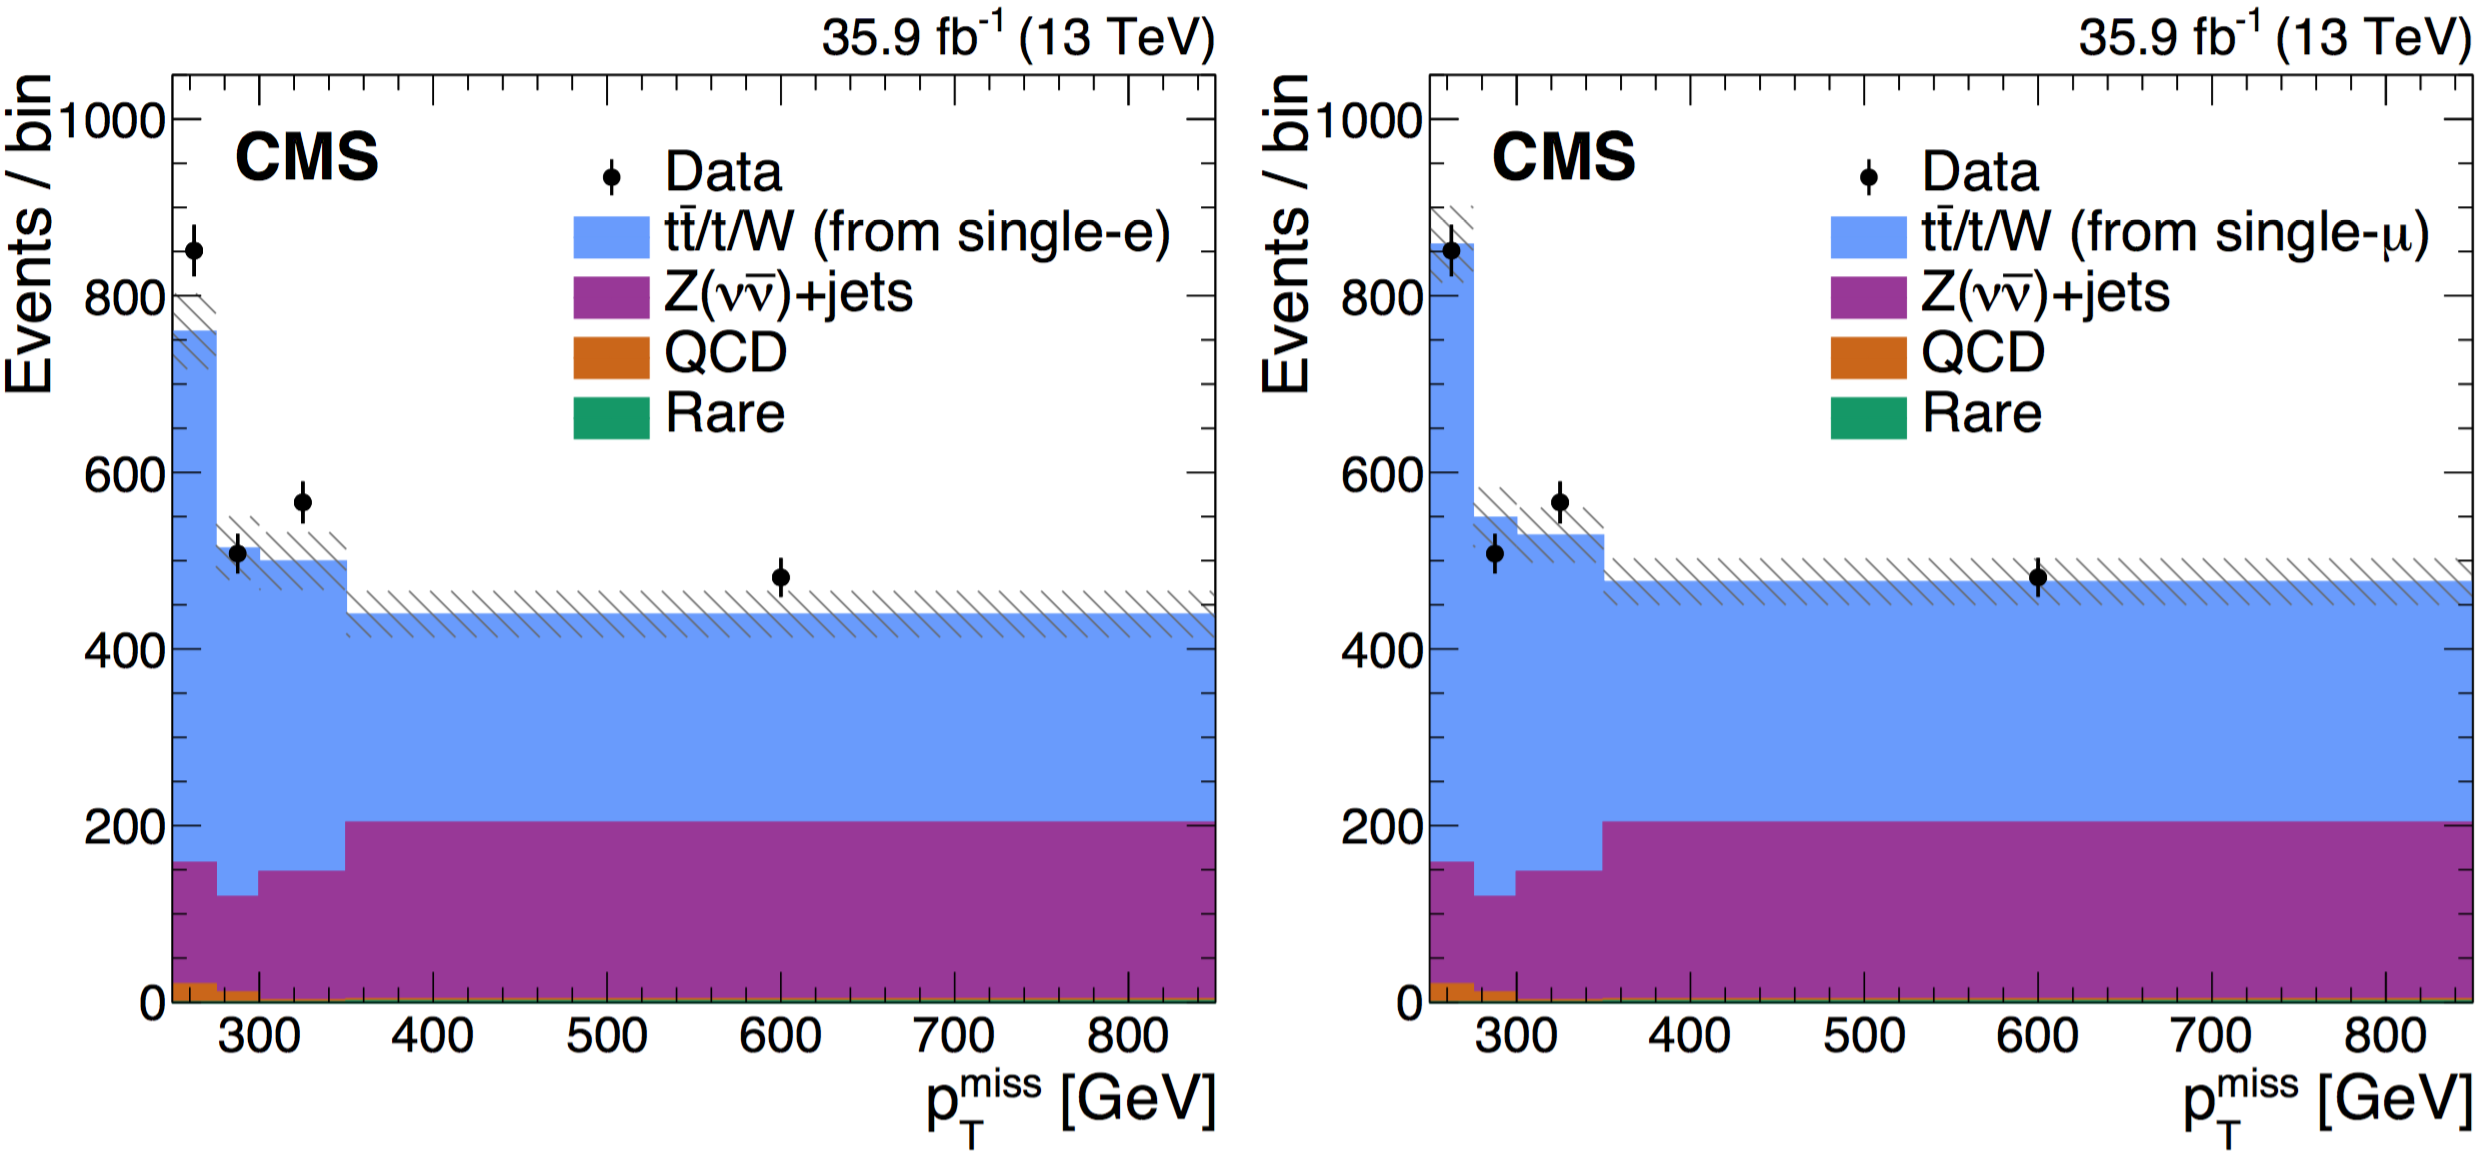
\includegraphics[width=0.8\textwidth]{LL.png} 
		\caption{Distribution of $p_{\text{T}}^{miss}$ for both the single-electron (left) and single-muon (right) SB data samples compared to predictions for SM processes. The hatched bands indicate the statistical uncertainties in the total SM prediction. Note that the data and the predictions for all backgrounds except that for t$\bar{\text{t}}$, single top quark, and W+jets events are identical between the left and right plots.}
		\label{LL} 
	\end{center}
\end{figure}

In order to test this method, a sideband (SB) region is selected which is orthogonal to the search region. This region is defined by the same selection criteria applied to data except for $N_t = 0$, $N_b \geq 2$, and $\Delta\phi$($p_{T}^{miss}$,  j$_\text{1,2,3,4}$)$~> 0.5$, where the last two requirements are applied in order to suppress contributions from Z($\nu\bar{\nu}$)+jets and QCD multijet processes. The SB is divided into four intervals of $p_{T}^{miss}$, where the contribution of lost-lepton and $\tau_\text{h}$ to the corresponding intervals are determined by multiplying the appropriate single -electron and single-muon CS (\autoref{LL}) by a translation factor from simulation. The contribution to the SB from other backgrounds, such as Z+jets, QCD multijet and rare events, is estimated directly from simulation. The total SM background prediction is found to agree with the data within uncertainty, confirming the validity of the translation factor procedure.\\

Systematic uncertainties stemming from the prediction of t$\bar{\text{t}}$, single top quark and W+jets background events are determined from various sources: The statistical uncertainty associated to the translation factors determined for each search region (1--40\%), the lepton reconstruction and isolation efficiency (7--43\%), the jet and $p_{\text{T}}^{miss}$ energy scale and resolution (maximum of 64\%), the ISR modeling (maximum of 13\%), the PDF's (maximum of 32\%) and the b-jet tagging efficiency (1\%).

\subsection{The Z $\rightarrow\nu\bar{\nu}$ Background}\label{ZnunuSection}

The Z $\rightarrow\nu\bar{\nu}$ background is derived using simulated Z $\rightarrow\nu\bar{\nu}$ events that have been corrected for observed differences between data and simulation. In order to correctly estimate this background two scale factors are used to weigh the simulated events: $R_{norm}$ and $S_{DY}( N_j)$  which correct the normalization of the simulation and the shape of the simulated $N_j$ distribution, respectively. These scale factors are calculated from the dimuon control region which includes events with two muons and no muon or isolated track veto. In the region where $81 < m < 101$ GeV, the two muons are treated as if they were neutrinos.\\

The first scale factor, $R_{norm}$, is computed by comparing the expected event yield in the dimuon control region from the Drell-Yan (DY) simulation with the observed event yield in data after subtraction of the other SM processes. The second scale factor, $S_{DY}$, depends on the number of jets ($N_j$) in the event and is also computed from the dimuon control region in which the signal region requirements on $p_\text{T}^{miss}$, $N_t$ and $m_\text{T2}$ are removed, and the $H_\text{T}$ requirement is relaxed to $H_\text{T} > 200$ GeV. For each $N_j$ bin this scale factor is calculated from the ratio between data and the DY simulation. Its value ranges between 0.6 and 1.1, depending on the $N_j$ bin.

\begin{figure}[H]
	\begin{center}
		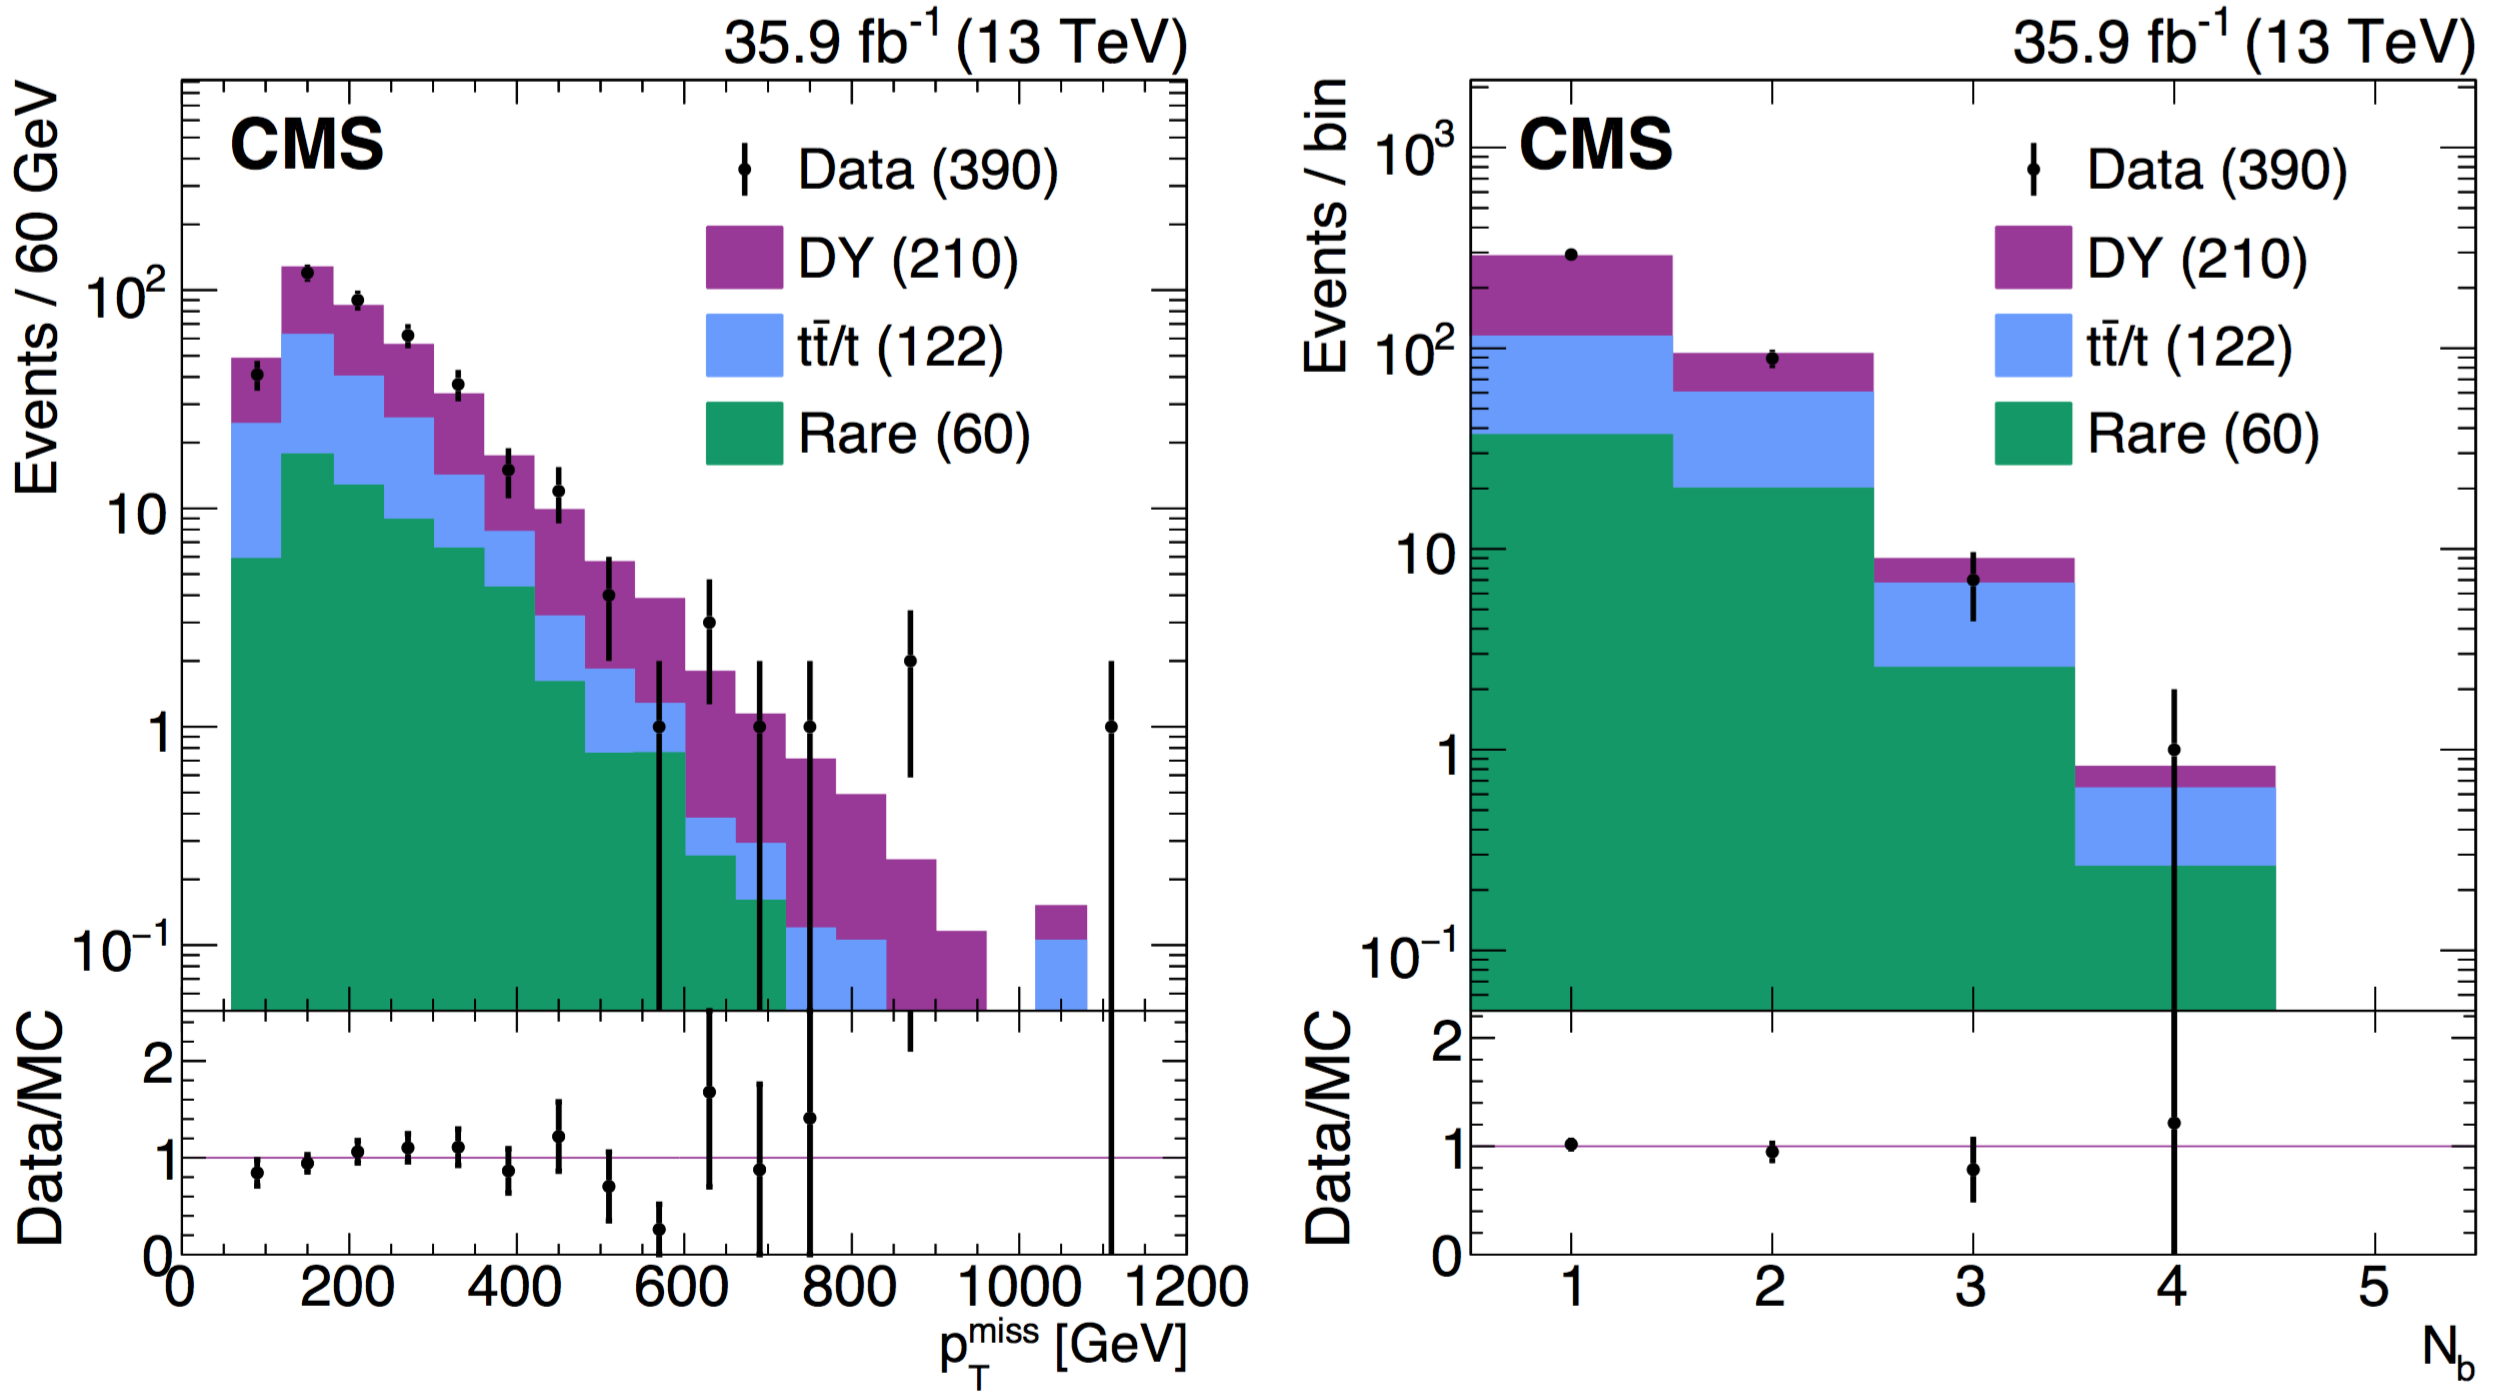
\includegraphics[width=0.8\textwidth]{Znunu.png} 
		\caption{The $p_\text{T}^{miss}$ (left) and $N_b$ (right) distributions of data and simulation in the loose dimuon CS after applying both the normalization and shape correction factors. The lower panels show the ratio between data and simulation. Error bars in the plot account only for statistical uncertainties. The values in parentheses indicate the integrated yields for each component.}
		\label{Znunu} 
	\end{center}
\end{figure}

The systematic uncertainties for the Z($\nu\bar{\nu}$)+jets background are obtained from the shape differences between data and simulation in the loose dimuon CS in terms of the $N_b$, $N_t$, $p_{\text{T}}^{miss}$, $m_\text{T2}$ and $H_\text{T}$ after the normalization factor ($R_{norm}$) has been applied. These include the statistical uncertainty in the $N_j$ shape correction (1--46\%) and in the overall normalization correction (7.6\%). Additional systematic uncertainties account for the jet and $p_{\text{T}}^{miss}$ energy scales (1--71\%), the b tagging efficiency (1--23\%), the PDFs and the renormalization and factorization scales (1--48\%), the statistical uncertainty in the simulation (1--81\%, with some search regions as high as 100\%), and the trigger (up to 14\%). An additional uncertainty is defined from the shift in the central value between the data and simulation in the distributions (14--44\% depending on the search region).

\subsection{The QCD Multijet Background}

To estimate the QCD Multijet background a signal-depleted, QCD multijet-rich data control sample is used. This control sample is defined by inverting the preselection requirements on $\Delta\phi$ ($p_\text{T}^{miss}$,  j$_\text{1,2,3}$) and subtracting contributions of other SM backgrounds, such as t$\bar{\text{t}}$, W+jets, and Z +jets. For t$\bar{\text{t}}$ and W+Jets the same methods (lost-lepton and hadronic $\tau$) are used to estimate the contributions for this QCD multijet-enriched control region. In the case of the Z $\rightarrow\nu \bar{\nu}$ background, simulation is used for its estimation due to its small number. Following that, a translation factor, partly determined by data and partly by simulation, is used to convert the number of QCD multijet events measured in the data control region into a QCD multijet prediction for each search region bin. This translation factor, called T$_\text{QCD}$,  is computed as the simulated ratio between the signal region and the inverted-$\Delta\phi$ control region, in bins of $p_\text{T}^{miss}$ and $m_\text{T2}$ where the bins are bounded in the same way as the signal bins.\\

The systematic uncertainty associated with the QCD multijet background for each search region is obtained as the difference between the event yield from simulation of QCD multijet processes and the prediction obtained by applying the background prediction procedure to simulated QCD multijet samples (30--500\%). Other sources include the statistical uncertainty in the translation factors (30--300\%) and the subtraction of the non-QCD-multijet SM contributions to the QCD control sample (2--50\%).

\subsection{Background From Rare and Other Processes}

The background contribution from rare processes forms only a tiny fraction of the overall SM background and has therefore a small effect on the final result. The estimation for these processes are determined directly from simulation, with the biggest contribution coming from t$\bar{\text{t}}$Z. With the exception of the t$\bar{\text{t}}$Z process, all other remaining backgrounds are combined. The comparison between simulation and the obtained data were found to be in agreement within a statistical uncertainty of 30\%, which is attributed to the systematic uncertainty in the estimation of the t$\bar{\text{t}}$Z background.

\section{Results and Interpretation}

\begin{figure}[H]
\begin{center}
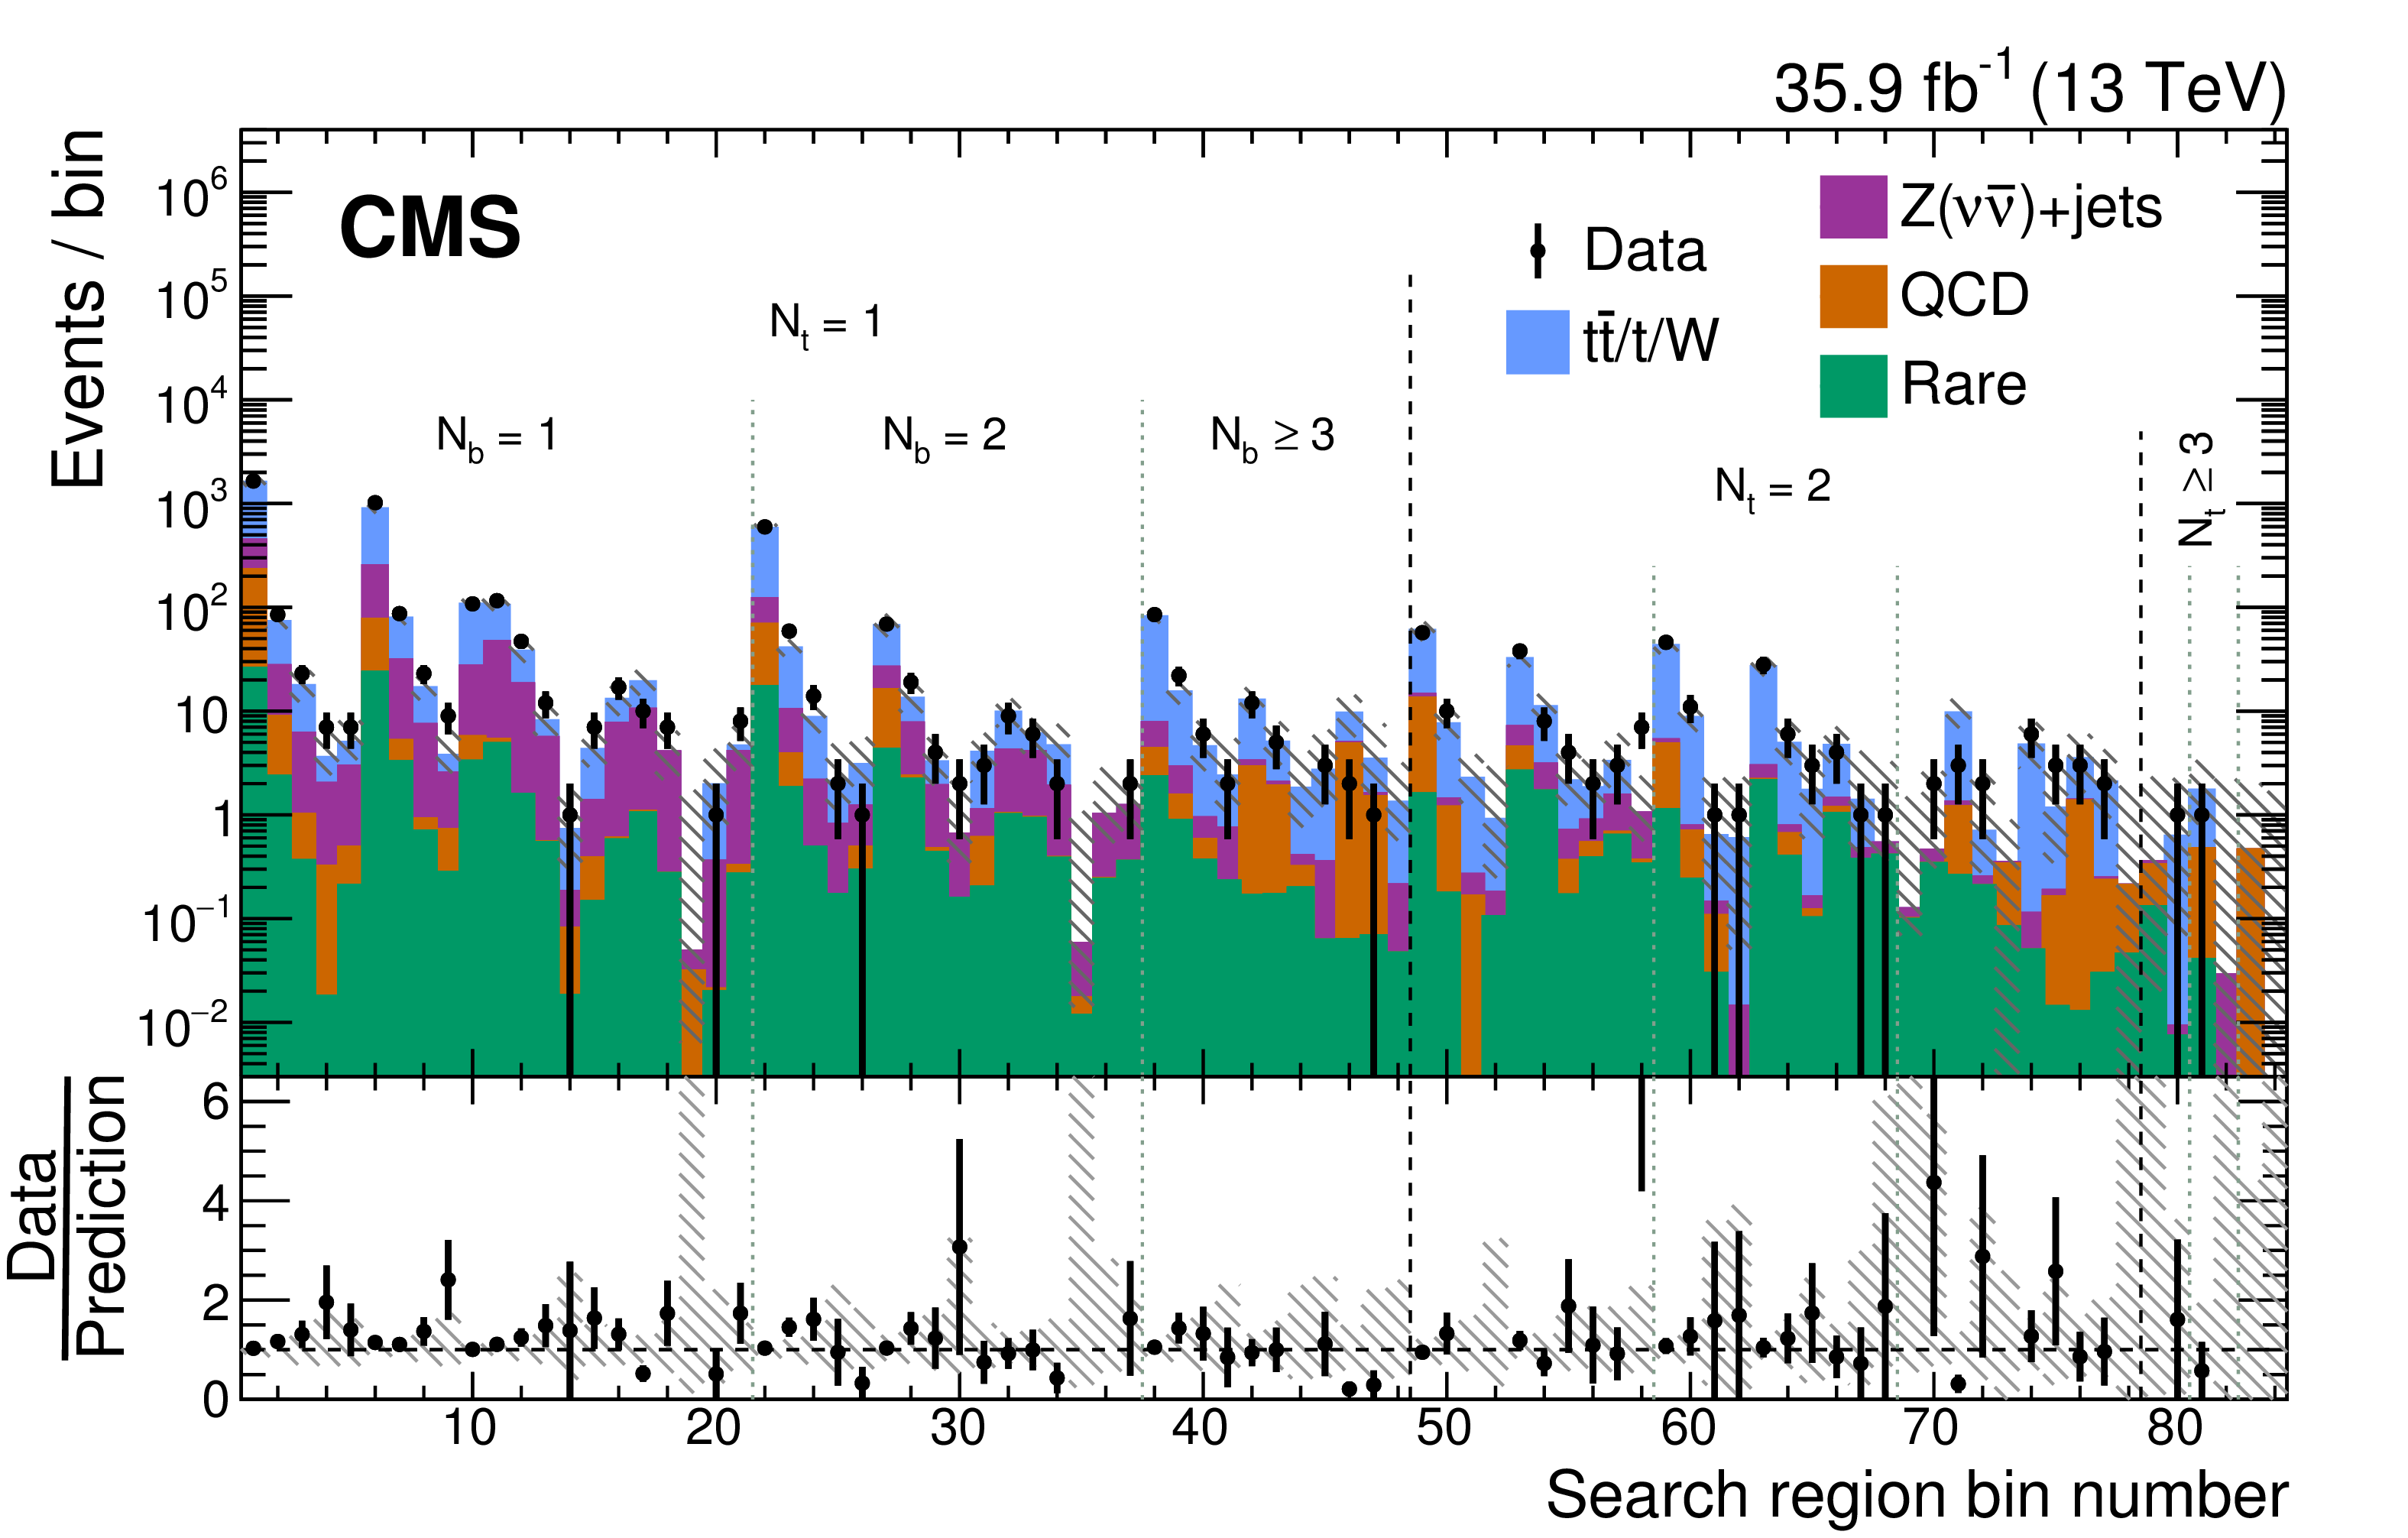
\includegraphics[width=0.8\textwidth]{SearchBinResults.png}  
\caption{Observed events compared to the corrected SM background predictions for all 84 search regions in the full data of 35.9 fb$^{-1}$ collected in 2016. The lower panel shows the ratio between the data and the total SM simulation. The gray bands show the total uncertainty related to the background prediction.}\label{SearchBinResults}
\end{center}
\end{figure}

\autoref{SearchBinResults} shows the summary of all observed events compared to the corrected SM background simulation for all of the 84 search bins. The data obtained shows no statistically significant deviation from the predicted SM background. The biggest contribution to the background is attributed to the t$\bar{\text{t}}$ and W+jets processes, followed by Z($\nu\bar{\nu}$)+jets, which could be dominant in regions that have a high $p_\text{T}$ threshold. The contributions arising from the QCD multijet and rare backgrounds are found to be nearly negligible in all of the search regions.\\

Exclusion limits are calculated for each of the signal models discussed in this chapter by applying a binned likelihood fit on the data. The likelihood function is obtained for each of the 84 search regions as well as for each of the background data control samples (single-electron, single-muon, and QCD) from the product of the Poisson probability density function. Exclusion limits were placed on the top squark, gluino and LSP production cross-sections with a 95\% confidence level (CL), calculated using a modified frequentist approach with the CL$_s$ criterion \cite{CL1,CL2} and asymptotic results for the test statistic\cite{stat1}.\\

\begin{figure}[H]
	\begin{center}
		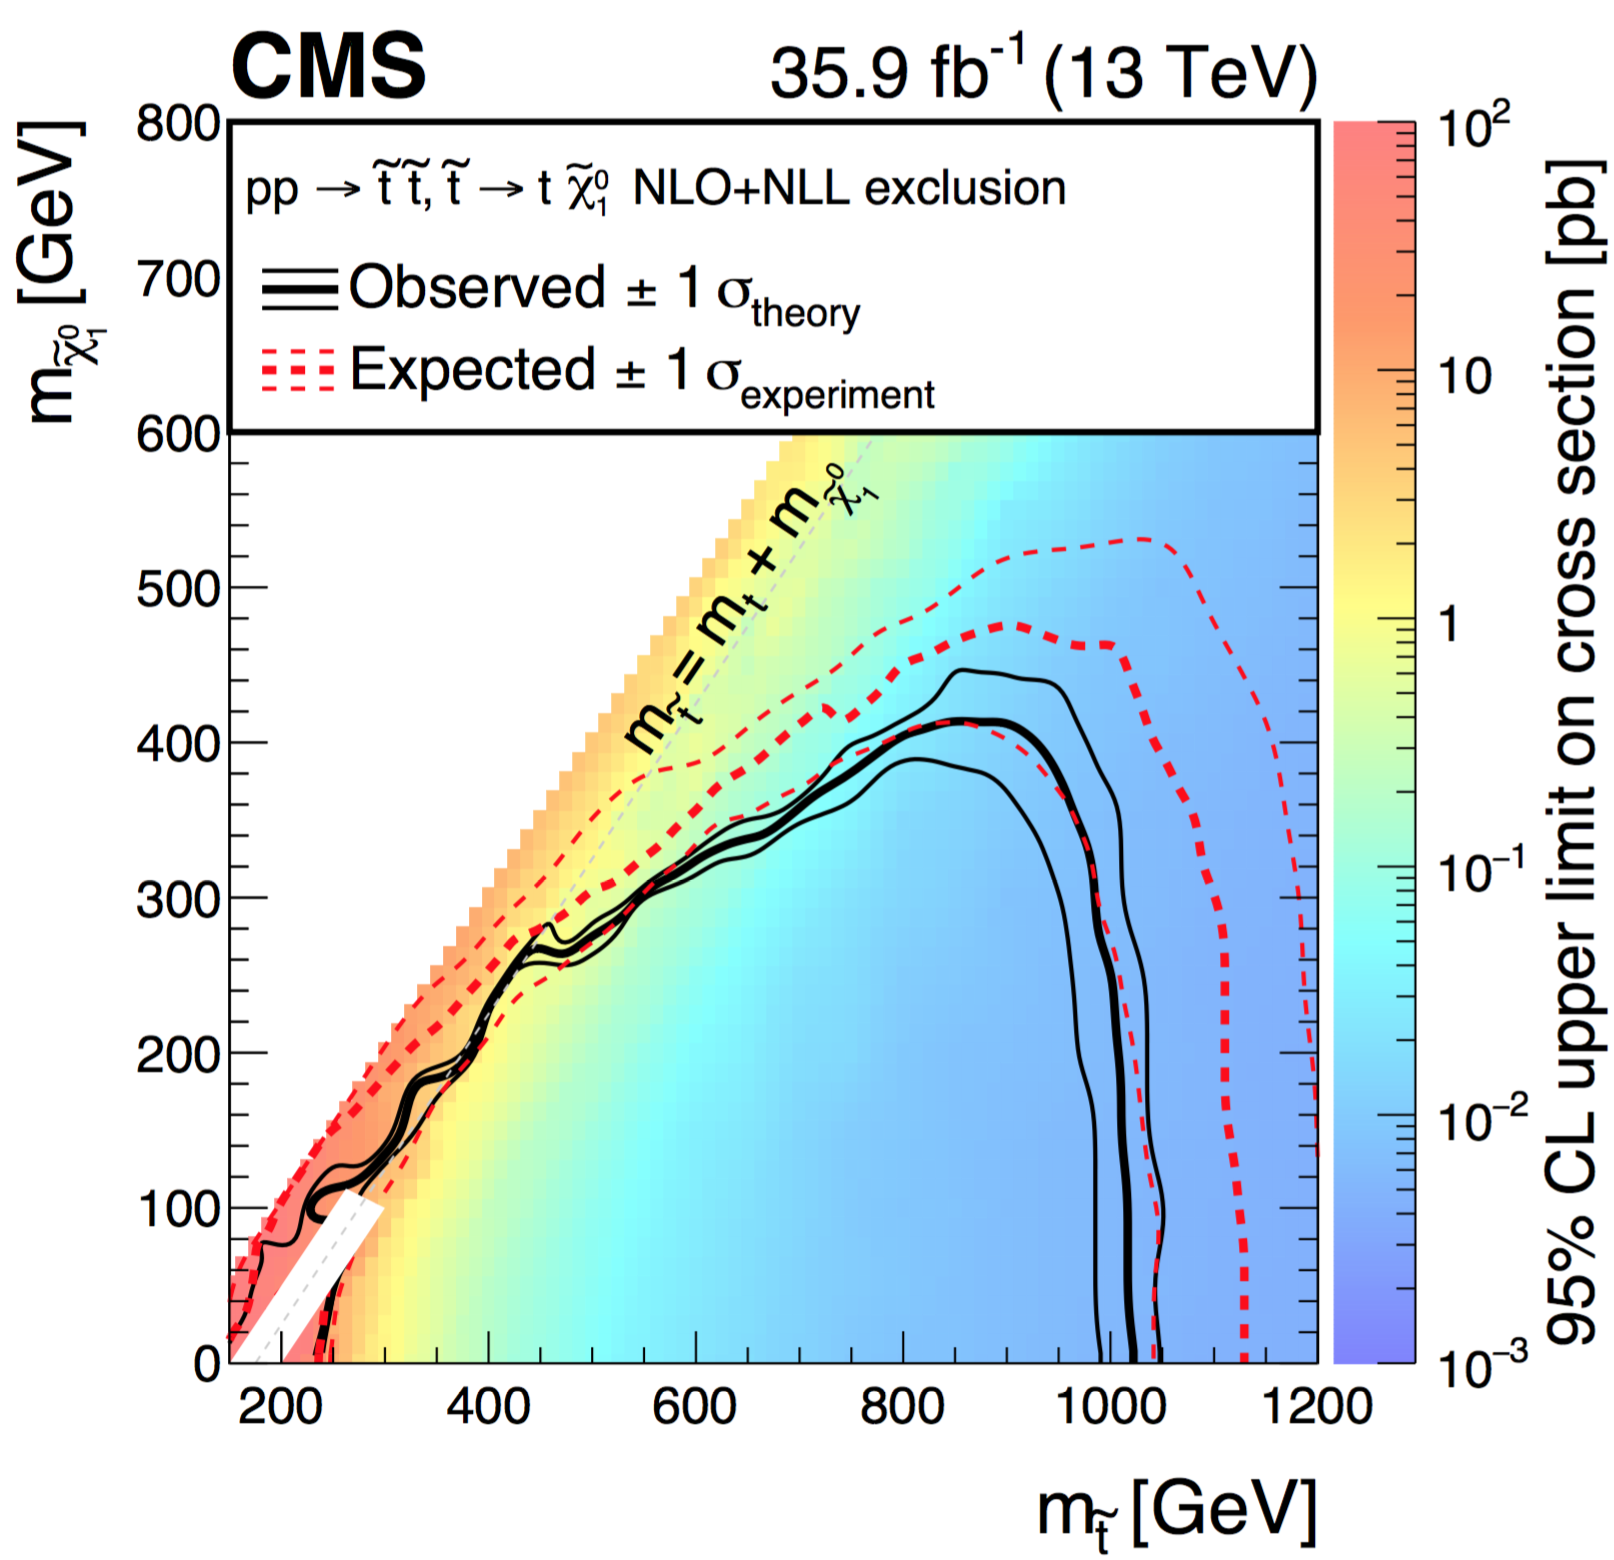
\includegraphics[width=0.55\textwidth]{T2ttLimit.png} 
		\caption{The 95\% CL upper limit on the production cross section of the T2tt simplified model as a function of the top squark and LSP masses. The solid black curves represent the observed exclusion contour with respect to NLO+NLL\cite{NLONLL} signal cross sections and the change in this contour due to variation of these cross sections within their theoretical uncertainties. The dashed
red curves indicate the mean expected exclusion contour and the region containing 68\% of the
distribution of expected exclusion limits under the background-only hypothesis.}\label{T2ttLimit}
	\end{center}
\end{figure}

The uncertainties from the search region modeling are taken into account for each of the 84 bins and arise from several different sources: the statistical uncertainty in the simulated event samples, the integrated luminosity (2.5\%\cite{Lumi}), the lepton and isolated-track veto efficiencies (up to 6.8\%), the b tagging efficiency (up to 21\%), the trigger efficiency (up to 2.6\%), the renormalization and factorization scales (up to 3.5\%), the ISR modeling (up to 46\%), the jet energy scale corrections (up to 34\%), the top quark reconstruction efficiency (up to 14\%), and the modeling of the fast simulation compared with the full simulation for top quark reconstruction and mis-tagging (up to 24\%). All of the uncertainties, with the exception of the statistical precision of the simulation, are taken to be fully correlated between the search regions. Contributions from signal contamination in the signal modeling are found to be only significant from the single-lepton control samples and negligible for the rest.\\

The 95\% CL exclusion limits obtained for the T2tt model (\autoref{T2ttLimit}), which consists of direct top squark production, excludes top squark masses up to 1020 GeV and LSP masses up to 430 GeV. Meanwhile, \autoref{Limits} shows the results for the gluino pair production models: T1tttt, T1ttbb, T5tttt, and T5ttcc. For the T1tttt model, gluino masses of up to 2040 GeV and LSP masses up to 1150 GeV are excluded, with corresponding limits of 2020 and 1150 GeV for the T1ttbb model, 2020 and 1150 GeV for the T5tttt model, and 1810 and 1100 GeV for the T5ttcc model. 

\begin{figure}[tb]
	\begin{center}
		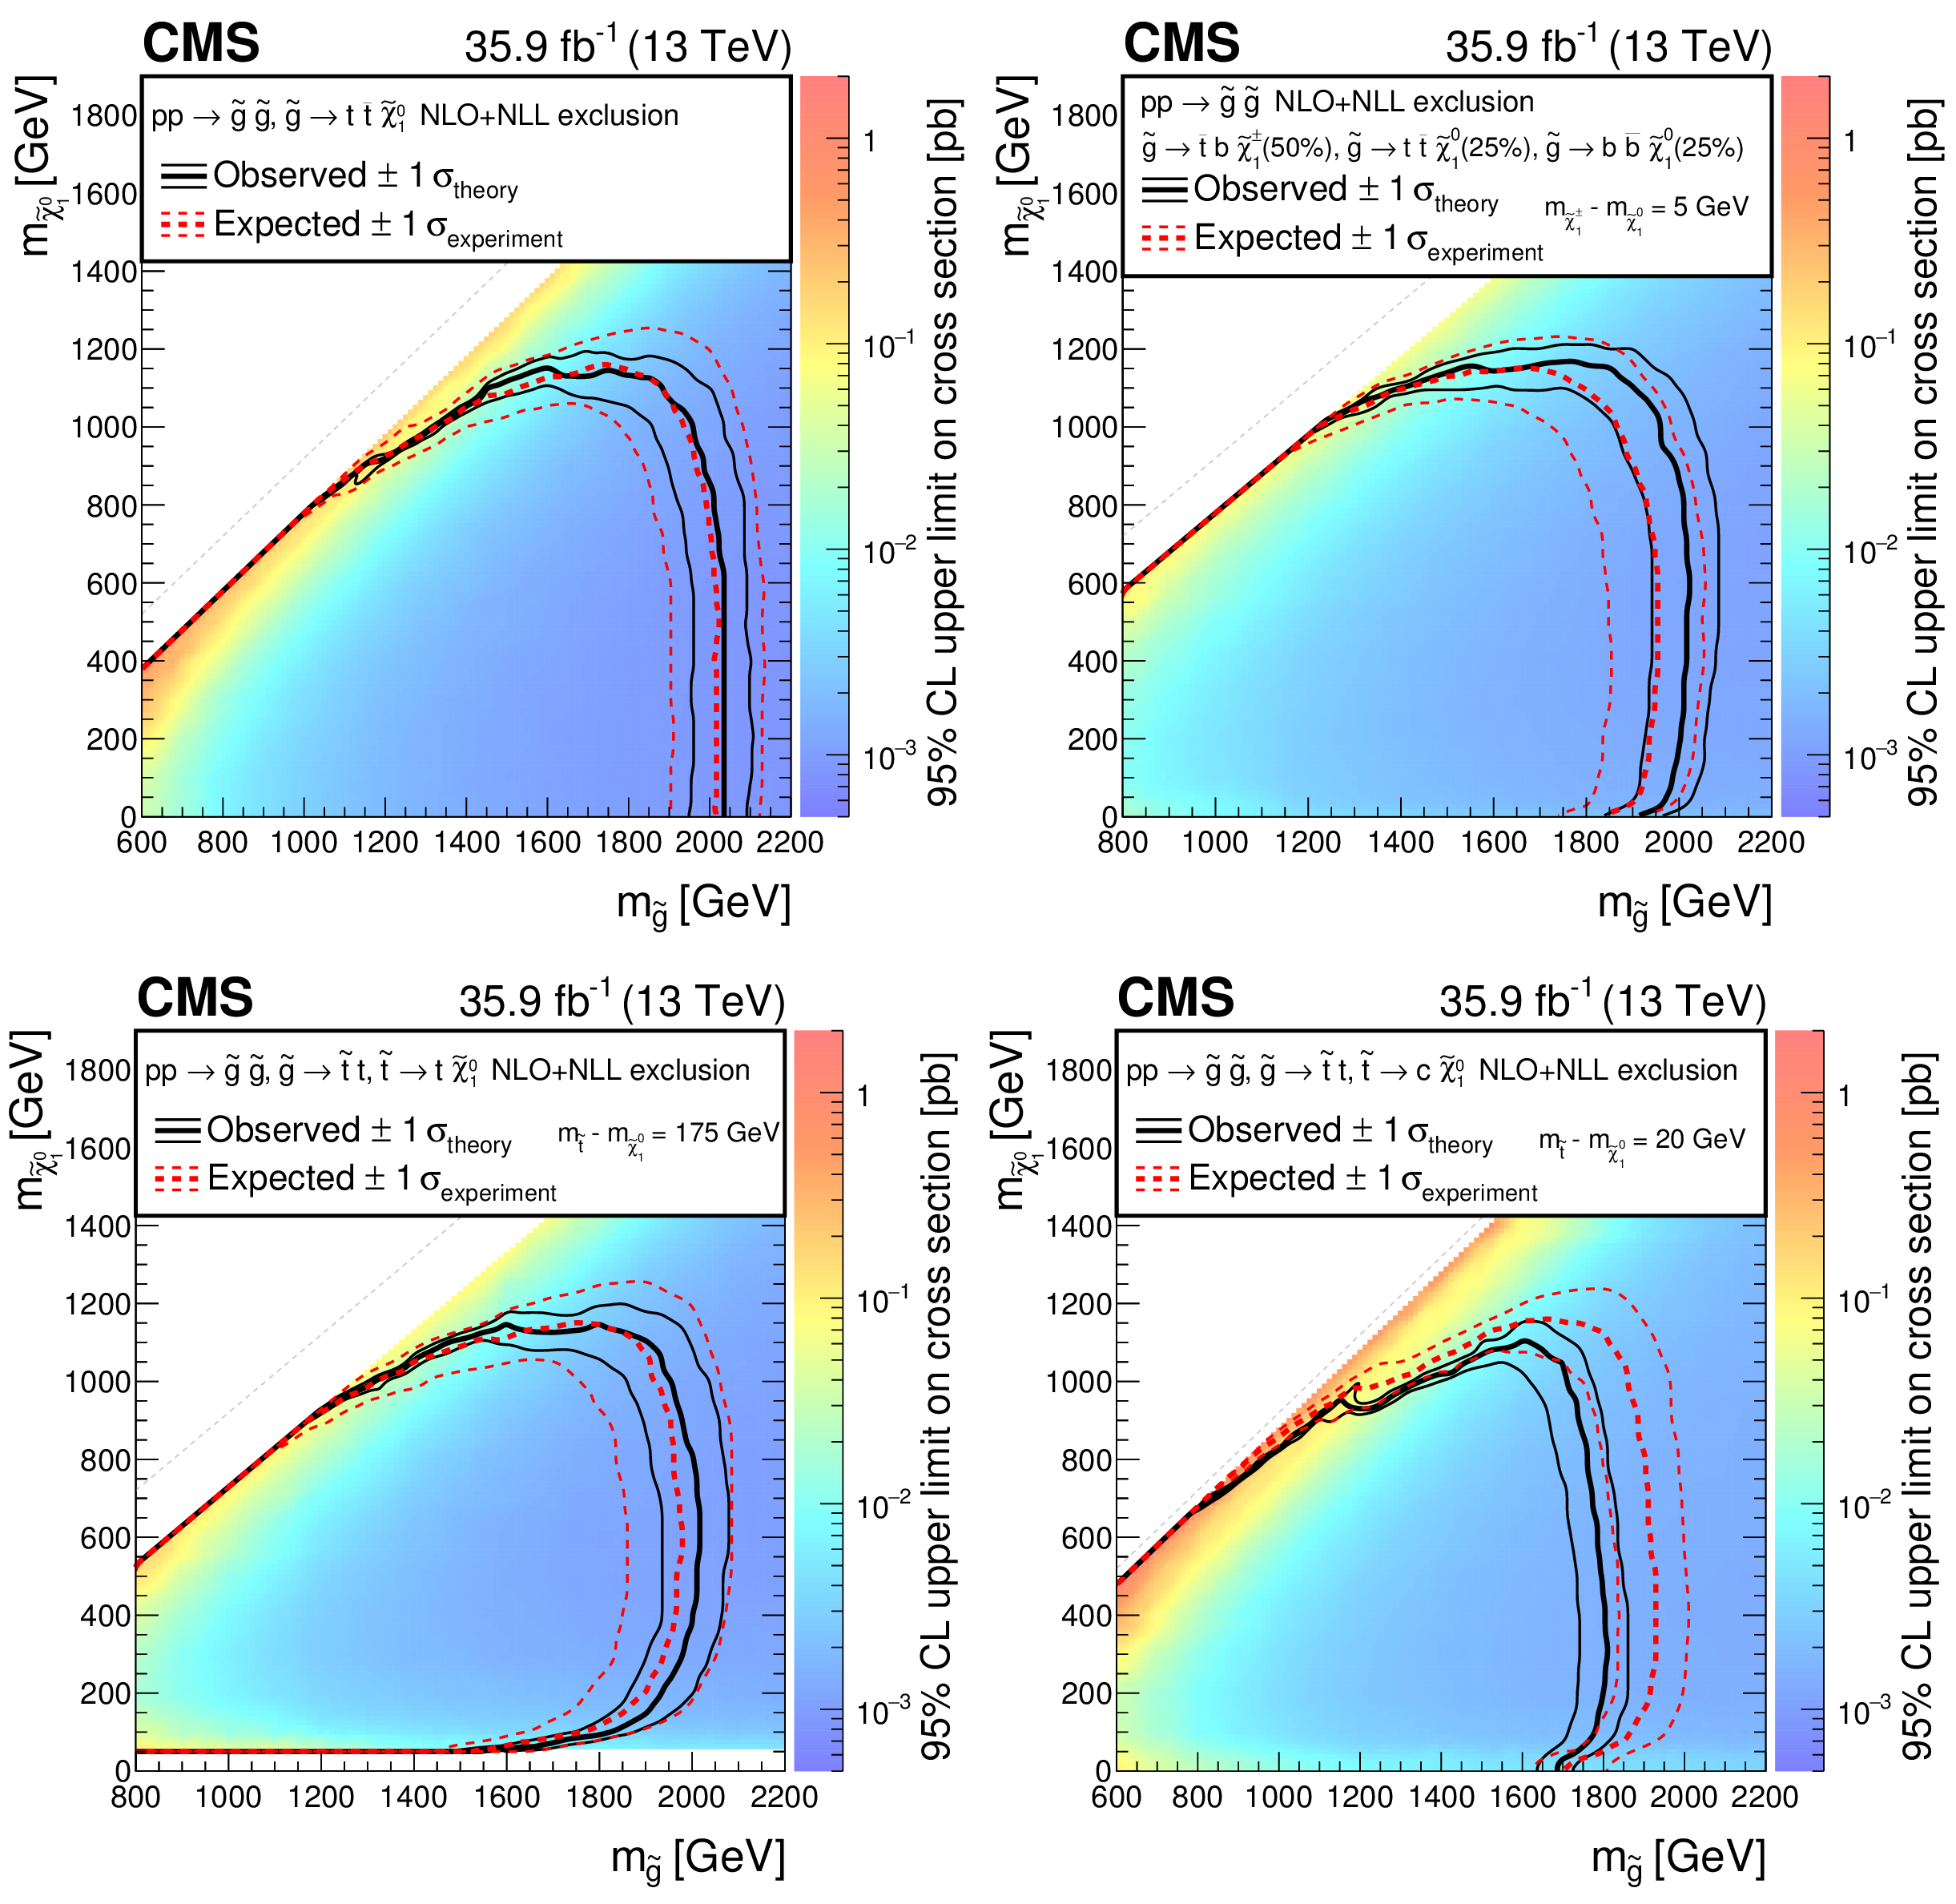
\includegraphics[width=1.0\textwidth]{Limits.png}
		\caption{The 95\% CL upper limit on the production cross section of the T1tttt (upper left), T1ttbb (upper right), T5tttt (bottom left), and T5ttcc (bottom right) simplified models as a function of the gluino and LSP masses.}\label{Limits} 
	\end{center}
\end{figure}



\chapter{Results \label{ch:results}}
Here first the limitations of Scikit-learn predefined ML models - Logistic Regression(LR) and Multi-Layer-Perceptron(MLP), are described. The Logistic Regression Model seems to work almost perfectly with all 3 classes when the bad region size is 5x5 (as in \autoref{Occupancymaps5x5}) with either the same or randomized location. When the bad region size is 1x1 like in \autoref{Ocuppancymaps1x1} the LR Model performs poorly with an accuracy of approximately 20\%.
 The MLP does not seem to work in any of the used cases that are studied as it always performs poorly with an accuracy of $\approx 40\%$.

\begin{figure}[h]
\centering
\begin{subfigure}[t]{.313\textwidth}
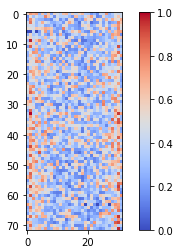
\includegraphics[width=\textwidth]{Good_image_1x1.png}
\caption{}
\end{subfigure}
\begin{subfigure}[t]{.3\textwidth}
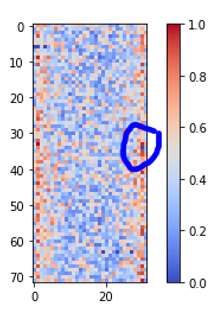
\includegraphics[width=\textwidth]{Dead_image_1x1.png}
\caption{}
\end{subfigure}
\begin{subfigure}[t]{.3\textwidth}
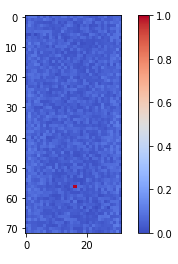
\includegraphics[width=\textwidth]{Hot_image_1x1.png}
\caption{}
\end{subfigure}
\vspace{1cm}
\caption{Occupancy Maps with 1x1 bad regions. A) Good image B) Dead image C) Hot image\label{Ocuppancymaps1x1}}
\end{figure}


d vice-versa. \autoref{IDtable} shows the cut values that are applied to photons that are found within both the ECAL barrel and endcap range. The associated values to the efficiency and the background rejection rate are shown for each of the three different photon ID selections.\\

In order to obtain the high efficiency and background rejection rae contributions.

\subsection{Photon Selection}\label{photonSelection}
The event selection process for the $\gamma$+jets control region starts with photon candidates that have a $p_\text{T} > 200$ GeV and are within the acceptance range of the CMS ECAL (given by $|\eta| < 1.4442$ for the barrel and $1.566 < |\eta| < 2.5$ for the endcaps). The photons are subjected to pass the loose ID/isolation cuts described in \autoref{photonID} in order to remove $\sim85\%$ of the background processes and obtain a prompt phototly improves the prompt photon selection by removing many of the events in the simulated samples where a lepton gets misidentified as a photon.

\begin{figure}[H]
\begin{center}
\begin{minipage}[b]{0.45\textwidth}
    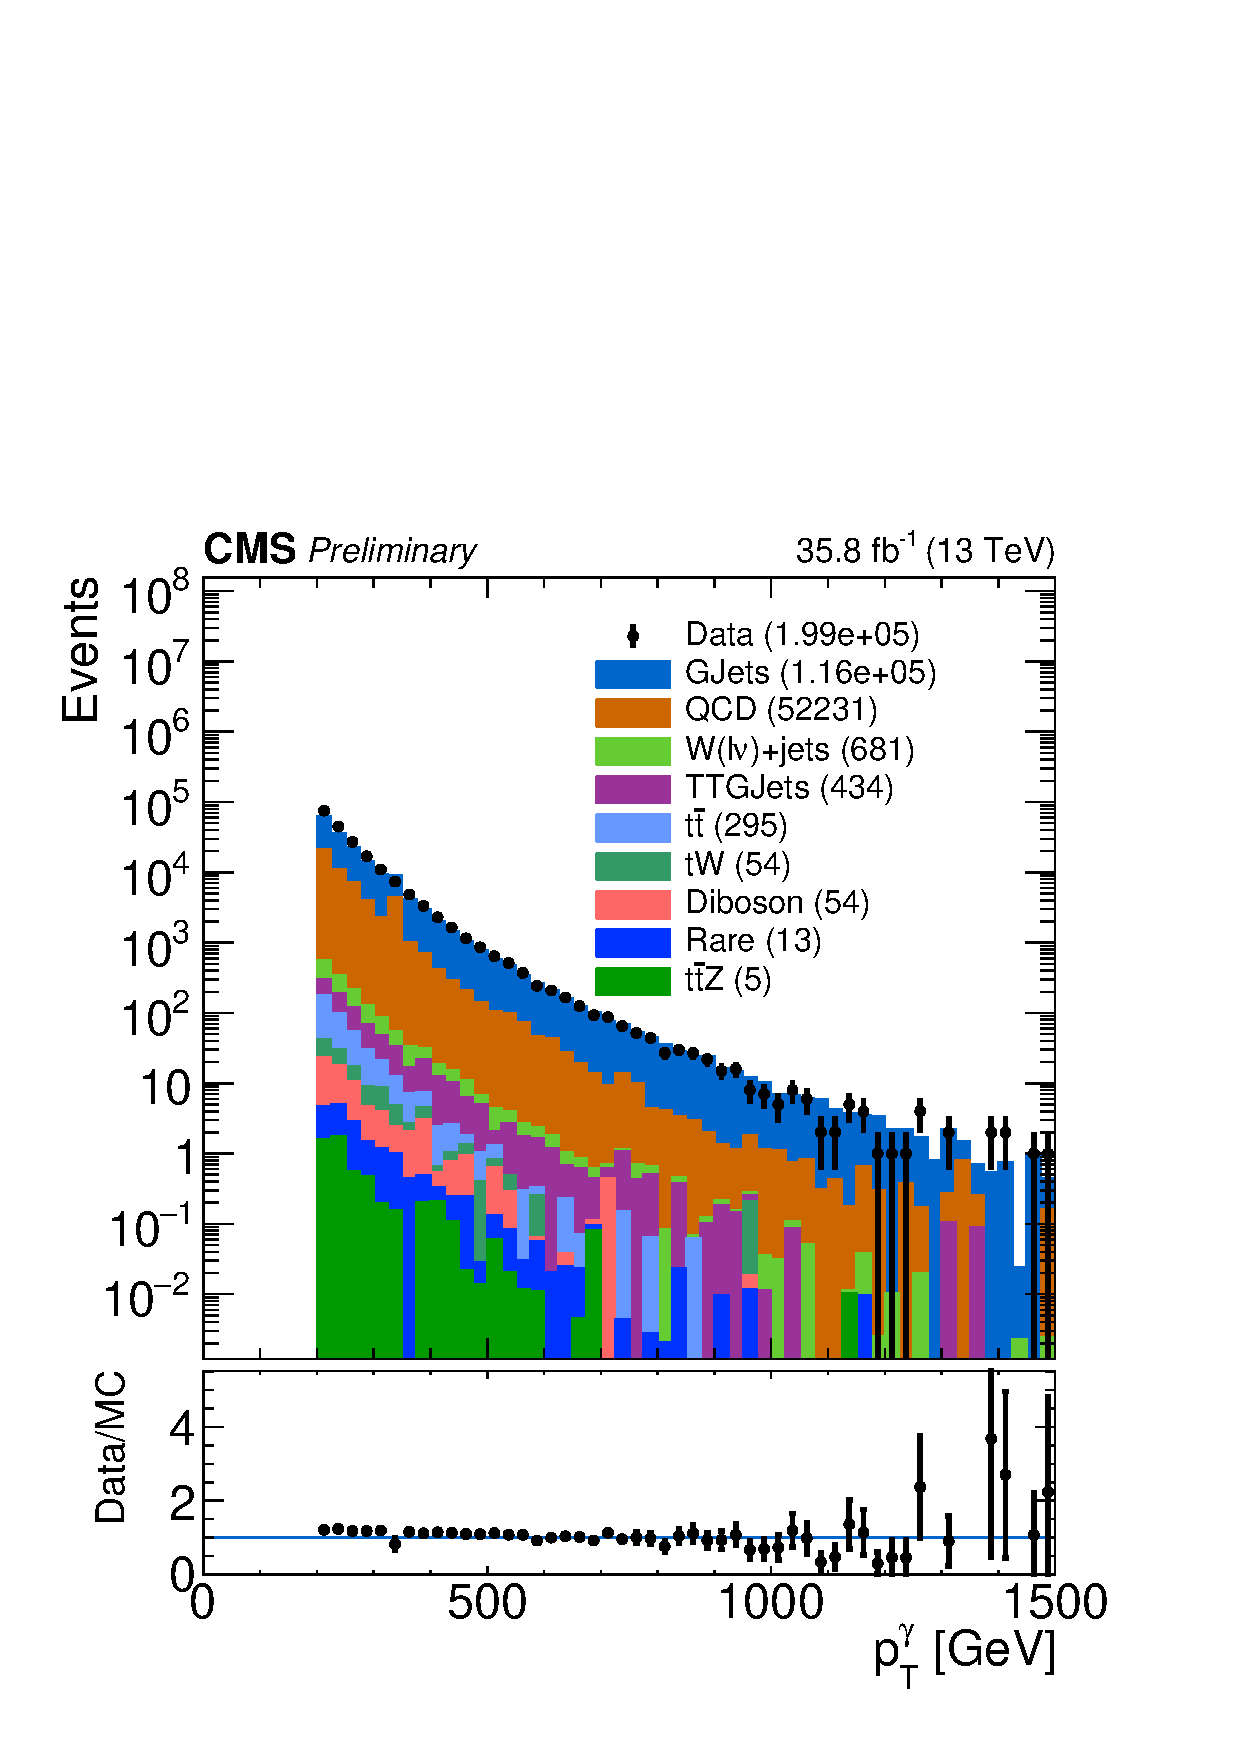
\includegraphics[width=\textwidth]{dataMC_PhotonPt_LooseLepVeto.pdf}
\end{minipage}
\begin{minipage}[b]{0.45\textwidth}
    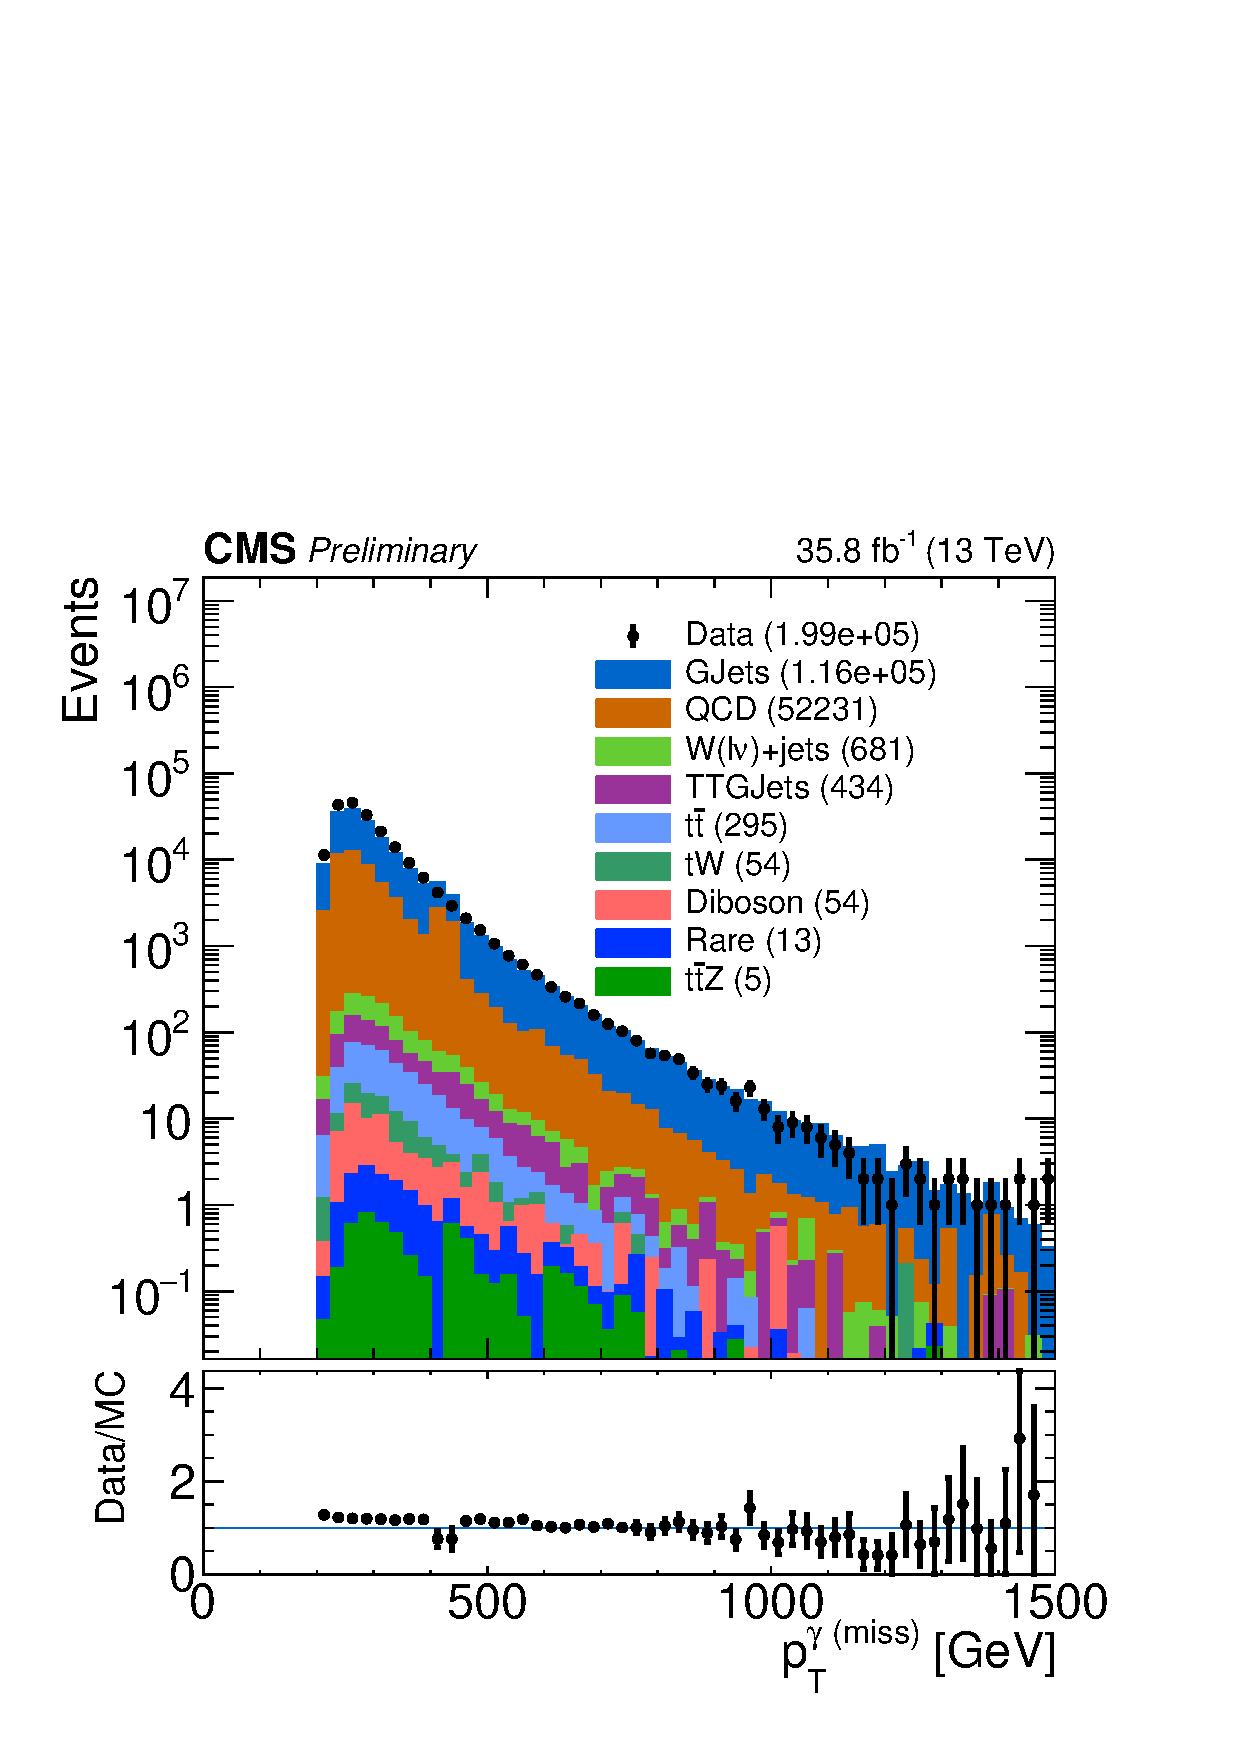
\includegraphics[width=\textwidth]{dataMC_MetGamma_LooseLepVeto.pdf}
\end{minipage}
\end{center}
\vspace{-1em}
\caption{Shown are both the $p_\text{T}^{\gamma}$ (left) and $p_\text{T}^{\gamma (miss)}$ (right) distributions before applying any corrections. $p_\text{T}^{\gamma (miss)}$ is obtained by adding the $p_\text{T}^{\gamma}$ to the total $p_\text{T}^{miss}$ in every event.}
\label{PtMetPt}
\end{figure}
\vspace{1em}

To further emulate the Z$\rightarrow\nu\bar{\nu}$+jets background, a variable in which the photons are treated as $p_\text{T}^{miss}$ is defined. We call this variable $p_\text{T}^{\gamma (miss)}$ and we obtain it by adding the $p_\text{T}^{\gamma}$ for every event to the total $p_\text{T}^{miss}$ in the event. Both the $p_\text{T}^{\gamma}$ and the resulting $p_\text{T}^{\gamma (miss)}$ distributions are shown in \autoref{PtMetPt} as data/MC comparison plots, where the simulated backgrounds are stacked in order of ascending contribution.\\

The main contributions from simulation arise from the $\gamma+$jets, QCD and to a lesser extent, t$\bar{\text{t}}\gamma$. Other non-dominant backgrounds in the control region include contributions from W($l\nu$)+jets, t$\bar{\text{t}}$, Diboson, tW, t$\bar{\text{t}}$Z and rare processes. Most of these lesser backgrounds are nearly negligible (several orders of magnitude lower than the dominant backgrounds) and are considered to be mostly composed of fake photons. In addition to the cuts described, all of the simulation samples are subjected to weights that apply corrections to pileup as well as the b-tagging efficiency. Data, on the other hand, is obtained from a sample that contains events with at least one identified photon. Photons in this sample are also subjected to the high-level trigger HLT\_Photon175, which restricts the selection to photons that have a $p_\text{T} >$ 175 GeV. Both simulation and data are subjected to the same selection criteria established in this section. 

\subsection{Photon Purity and Fake Rate}\label{purity&fakerate}

Three different types of photons make up the $\gamma+$jets CS: prompt photons, produced either directly or through fragmentation, and fake photons. Prompt photons are defined as photons which are formed shortly after the proton-proton collision (i.e. before the produced quarks and gluons have had enough time to form hadrons). Two types of photons fit in this category. The first type, which we designate as direct photons, are photons that are produced directly from the proton-proton interaction\cite{promptPho}. A secondary type of prompt photon, that is virtually indistinguishable from the direct photons at the detector level, originates from the decay of $\pi^0$ mesons and are called fragmentation photons. The final type of photon found in the CS corresponds to fake (or non-prompt) photons. The fake photon contribution typically arises from leptons (mostly electrons) whose tracks are not properly reconstructed, yet leave energy measurements in the ECAL.

\begin{figure}[H]
\begin{center}
\begin{minipage}[b]{0.49\textwidth}
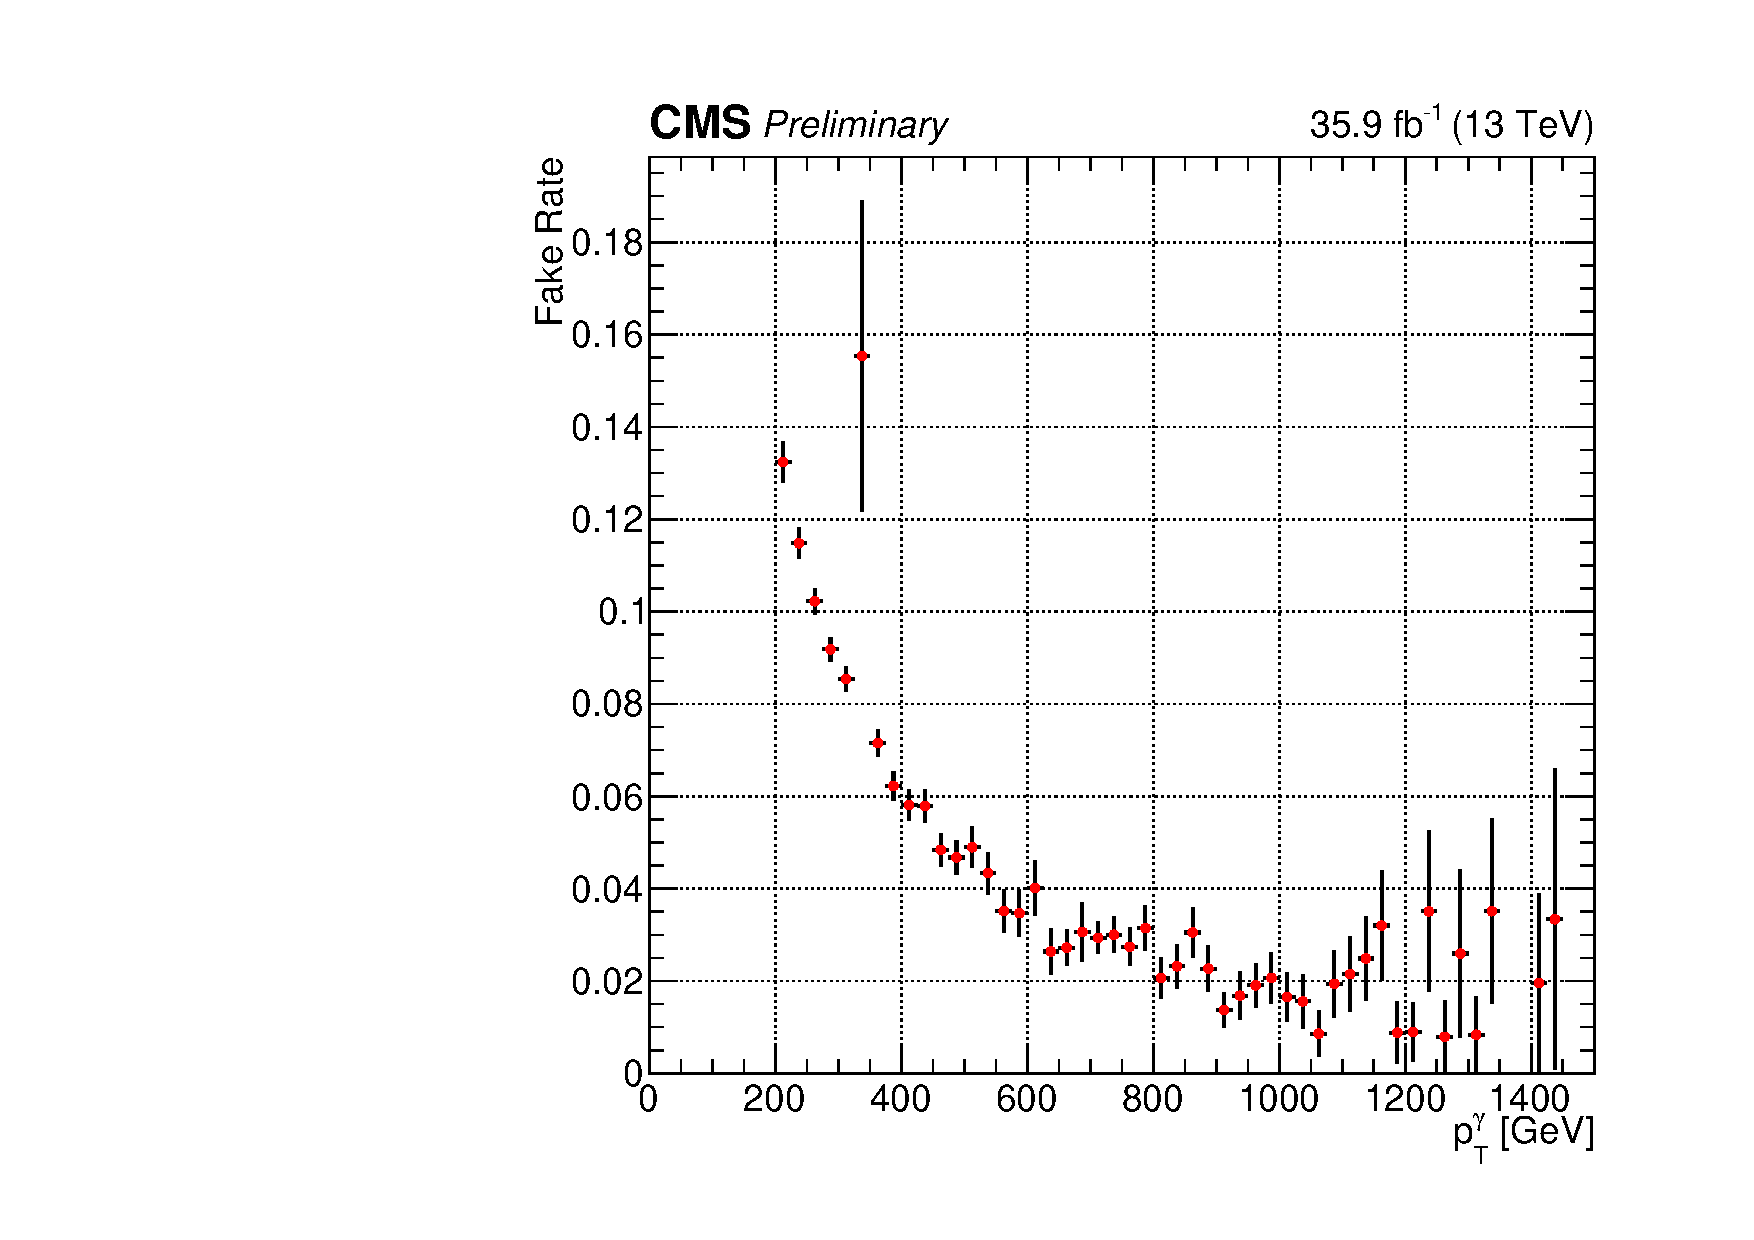
\includegraphics[width=\textwidth]{FakeRate_empty.pdf}
\end{minipage}
\begin{minipage}[b]{0.49\textwidth}
    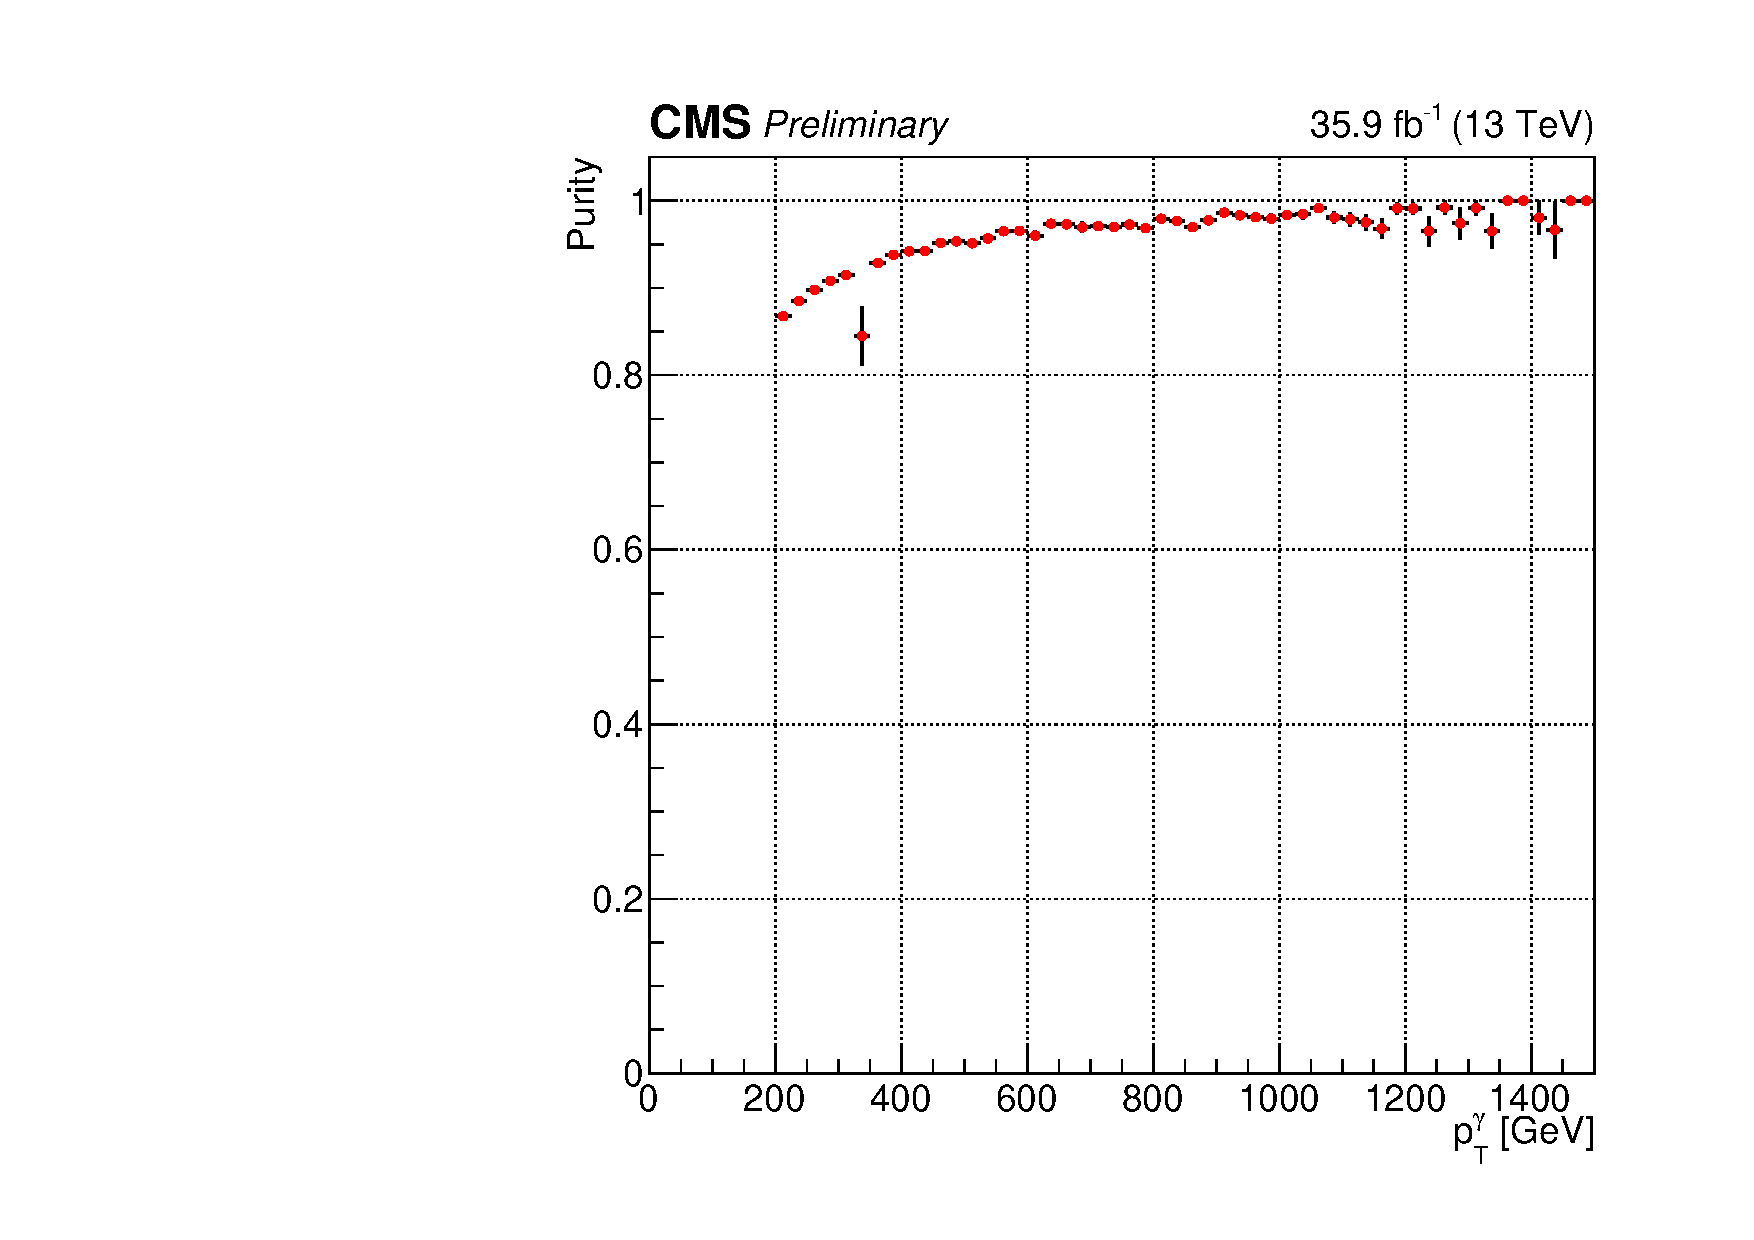
\includegraphics[width=\textwidth]{Purity_empty.pdf}
\end{minipage}
\end{center}
\vspace{-1em}
\caption{Plots for Fake Rate (left) and Purity (right) as a function of the photon $p_\text{T}$ are shown. The events are selected are required to have a $p_\text{T} > 200$ GeV, be within the ECAL acceptance range, and pass the loose ID selection cuts. This selection was produced in order to verify the values given by the E/$\gamma$ POG. As can be seen, the efficiency (purity) is seen to agree with the values of the loose photon ID/isolation selection.}
\label{FakeRatePurityLoose}
\end{figure}

\begin{figure}[H]
\begin{center}
\begin{minipage}[b]{0.49\textwidth}
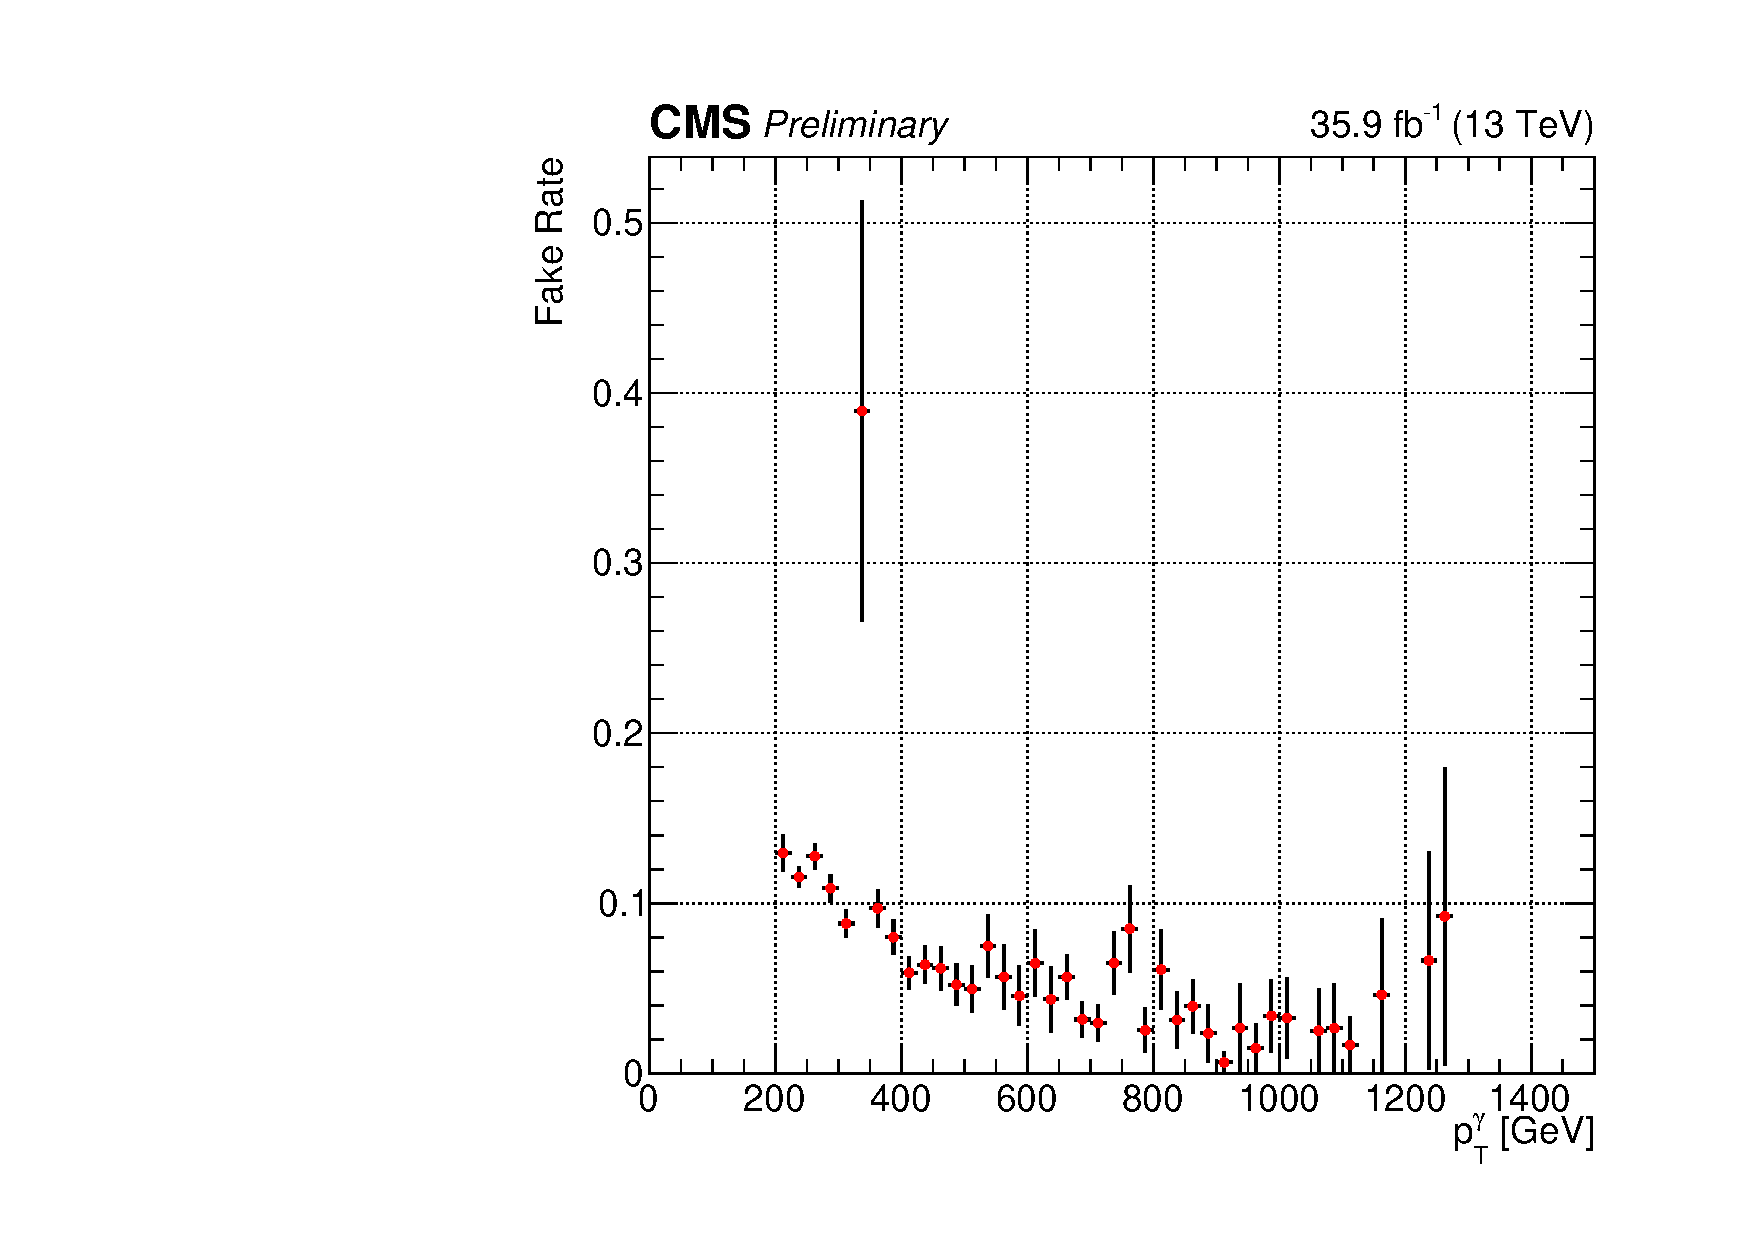
\includegraphics[width=\textwidth]{FakeRate_LooseLepVeto.pdf}
\end{minipage}
\begin{minipage}[b]{0.49\textwidth}
    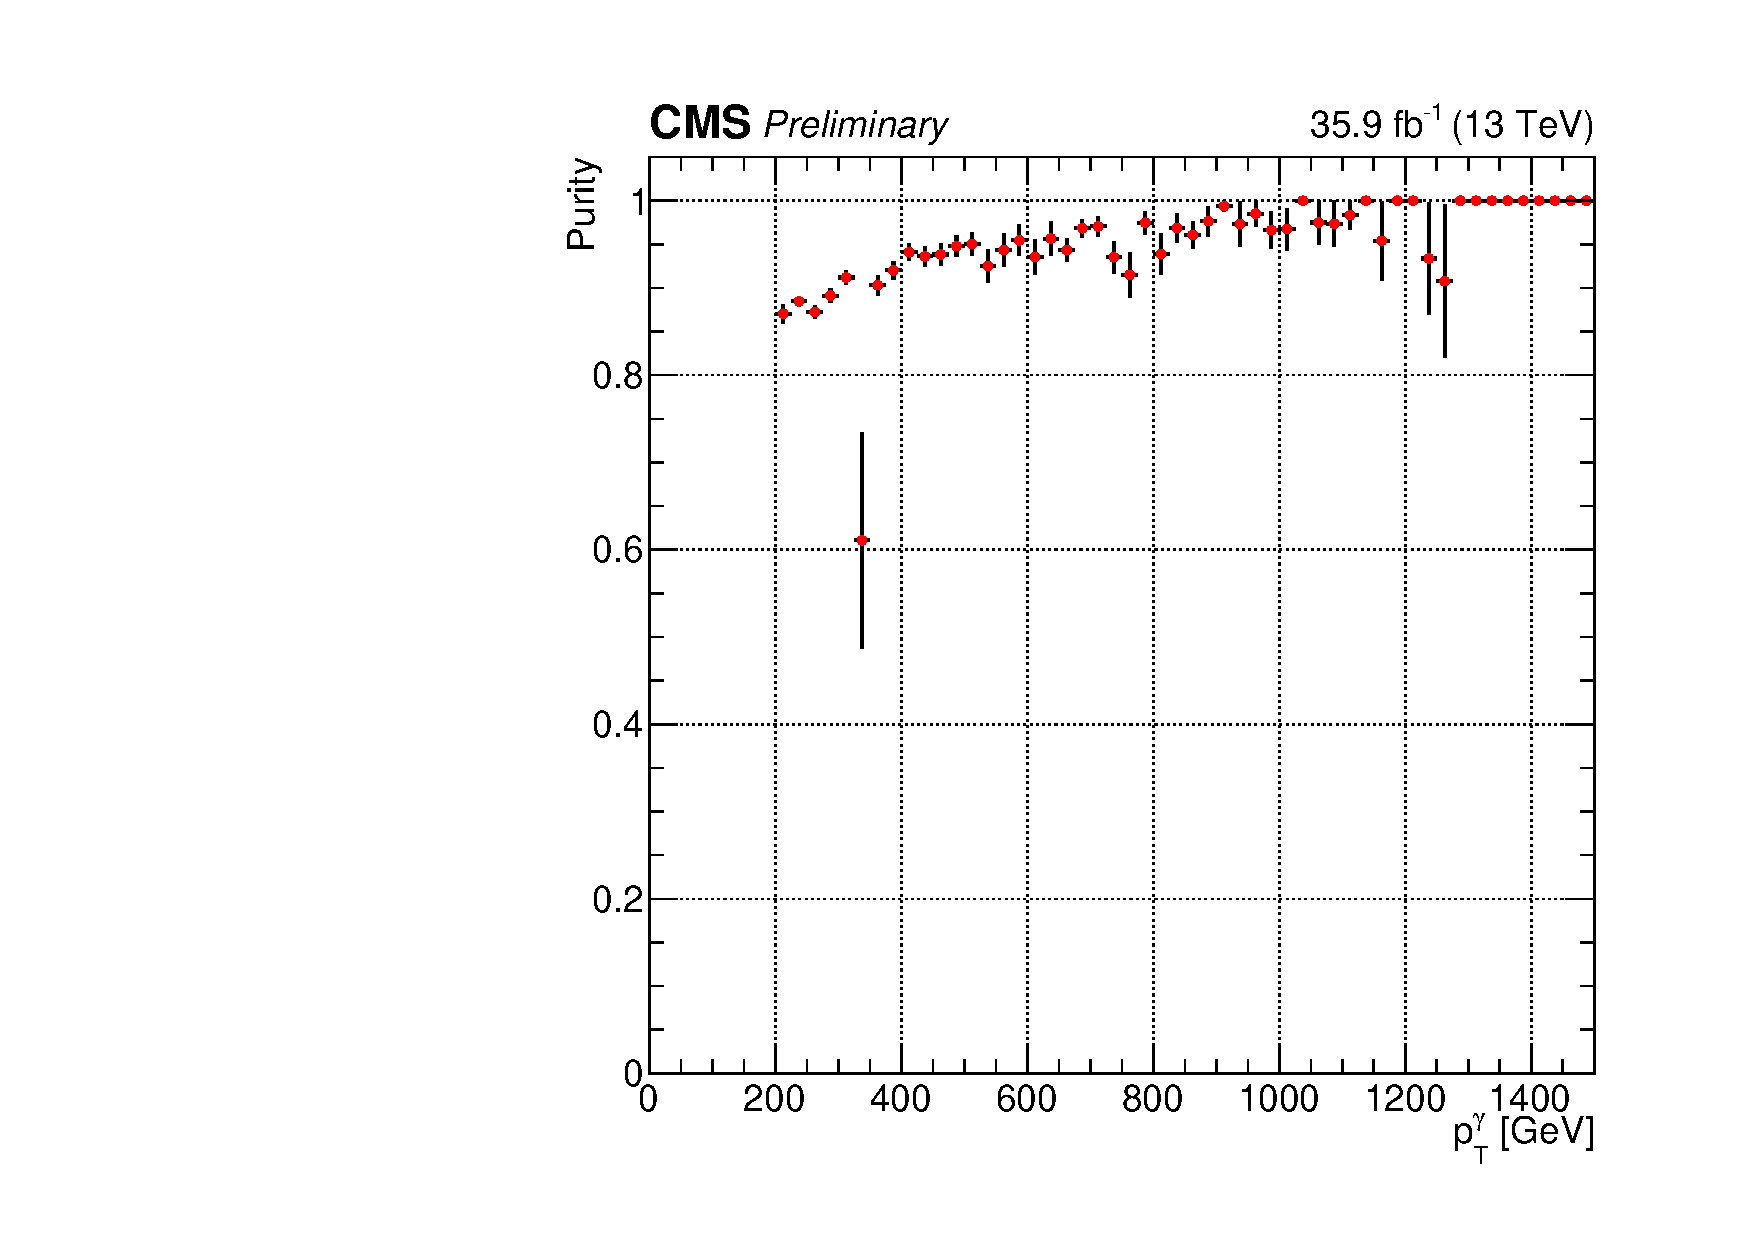
\includegraphics[width=\textwidth]{Purity_LooseLepVeto.pdf}
\end{minipage}
\end{center}
\vspace{-1em}
\caption{Plots for Fake Rate (left) and Purity (right) as a function of the photon $p_\text{T}$ are shown. These plots include photons with the full control region selection. Aside from exhibiting lower statistics, the plots seem to agree with the fake rate and purity before all the control region cuts are applied.}
\label{FakeRatePurityCR}
\end{figure}

\vspace{1em}

In order to identify prompt photons, reconstructed photons from the $\gamma+$jets and QCD samples are matched to generator-level photons in space and momentum by requiring $\Delta R(\gamma_\text{gen},\gamma_\text{reco}) < 0.4$ and $0.5 < p_\text{T}^\text{gen}/p_\text{T}^\text{reco} < 2.0$, respectively. Any reconstructed photon which fails to get matched to a generator level photon is labeled as a fake/non-prompt photon. Direct photons are identified by further requiring that the reconstructed photons be matched to a parton (a gluon or quark) in space as $\Delta R(\gamma,\text{parton}) > 0.4$. This requirement is intended to distinguish the reconstructed photons from highly boosted $\pi^0$'s, which compose a large portion of the experimentally indistinguishable fragmentation photons. Finally, fragmentation photons are obtained exclusively from QCD simulation and are required to have $\Delta R(\gamma,\text{parton}) < 0.4$ in order to avoid double counting photons from the $\gamma+$jets sample.\\

With all three types of photons defined, a study can be carried out from simulation to estimate their respective contributions to the defined control region. The study takes into account that any reconstructed photon in the $\gamma+$jets or QCD samples can only be categorized as prompt (through direct production or fragmentation) or non-prompt (fake). The purity and fake rate can then be defined in terms of the relative proportions of prompt or non-prompt photons with respect to the sum of the contributions from all three types of photons. Identified direct photons are taken from the $\gamma+$jets sample exclusively. Meanwhile, the fragmentation and fake photon contributions are taken from the QCD sample. The three quantities are then added together and their respective contributions are determined in terms of the photon $p_\text{T}$ (\autoref{FakeRatePurityLoose}).\\

The photon purity (\autoref{FakeRatePurityLoose} and \autoref{FakeRatePurityCR}, right) is defined in terms of the prompt and non-prompt photons as:\\

\begingroup
	\large
	\begin{center}
	%\begin{equation}
		$p_\gamma = \frac{prompt}{prompt+fake}$ ,
	\end{center}
	%\end{equation}
\endgroup
\vspace{1em}

\noindent{where the prompt photon portion comes from the sum of the direct photons (extracted from the $\gamma$+ jets sample) and the fragmentation photons (extracted from the QCD sample). The remaining non-prompt (or fake) photons all come from photons in the QCD sample that were not matched to truth-level photons in space and momentum with the specified required conditions. Meanwhile, the photon fake rate (\autoref{FakeRatePurityLoose} and \autoref{FakeRatePurityCR}, left) is defined from this same combination of samples as:}\\

\begingroup
	\large
	\begin{center}
	%\begin{equation}
		$f = \frac{fake}{prompt+fake}$ ,
	\end{center}
	%\end{equation}
\endgroup
\vspace{1em}

\autoref{FakeRatePurityLoose} shows the purity and fakerate for photons that pass the loose ID/selection, have a $p_\text{T} > 200$ GeV and are within the ECAL acceptance range. A sample is obtained in which 77\% of the photons are direct, 12\% are fragmentation and 11\% are fakes. This implies an average purity of $\sim$89\% for this sample, well within the value that is expected. \autoref{FakeRatePurityCR} shows the same ratios for the loose $\gamma$+ jets control region described in \autoref{photonSelection}. Although the amount of statistics has decreased due to the additional cuts, a similar trend can be observed.

\section{The Z$\rightarrow\mu^{+}\mu^{-}$ Control Region}

The Z$\rightarrow\mu^{+}\mu^{-}$ control region defined in this section is in every respect identical to the one applied in the 2016 analysis (\autoref{ZnunuSection}. The only difference between the 2016 method and the one discussed in this chapter is that the Drell-Yan (DY) sample is only used for the normalization correction of the Z$\rightarrow\nu\bar{\nu}$ background. Therefore, the loose $\mu\mu$ control region is not used or applied in the calculation of the scale factors. In the following subsections only the tight $\mu\mu$ control region, and its usage to obtain the normalization scale factor $R_{norm}$, is discussed.

\subsection{Muon ID and Isolation}

The muons are selected using the ``medium muon'' selection\cite{muonID}, per the recommendation of the muon POG. The muon candidates in this selection satisfy $p_\text{T} > 10$ GeV and $|\eta| < 2.4$. Other additional cuts are applied to aid in the muon candidate selection, such as an impact parameter cut. Muons are also subjected to a PF relative-isolation (also referred to as mini-isolation) in which the cone size is inversely proportional to the muon $p_\text{T}$. This requirement enforces the $p_\text{T}$ within the isolation cone to be at most 20\% of the muon $p_\text{T}$ in order to eliminate events with an isolated muon. Details of the medium photon selection are included in \autoref{table1muons} and \autoref{table2muons}, while details of the impact parameter cut are summarized in \autoref{table3muons}.

\begin{table}[H]
\begin{center}
\includegraphics[width=0.6\textwidth]{table1muons}
\caption{Muon Medium ID 2016 HIP Safe}
\label{table1muons}
\end{center}
\end{table}

\begin{table}[H]
\begin{center}
\includegraphics[width=0.4\textwidth]{table2muons}
\caption{Muon Medium ID HIP Safe Good Global Muon}
\label{table2muons}
\end{center}
\end{table}

\begin{table}[H]
\begin{center}
\includegraphics[width=0.3\textwidth]{table3muons}
\caption{Additional Impact Parameter cut on Muons}
\label{table3muons}
\end{center}
\end{table}

\subsection{Muon Selection in the Tight Control Region}\label{tightmumu}

Events are selected from data samples that contain exactly two oppositely charged muons ($\mu^{+}\mu^{-}$), which fall within the invariant mass $81 < m_{ll} < 101$ GeV window for the Z boson. Additional cuts for the tight muon selection include baseline requirements such as an $H_\text{T} > 300$ GeV, $N_j \geq 4$, the $\Delta\phi$ baseline cut on leading jets, a $p_\text{T}^{miss} > 250$ GeV, an $m_\text{T2} > 200$ GeV and at least 1 top-tagged jet $N_t \geq 1$. In addition, the $p_\text{T}$ of the two muons are required to be $p_\text{T} > 50$ GeV for the leading muon and $p_\text{T} > 20$ GeV for the sub-leading one. The only difference, when compared to the signal region is the missing lepton veto, in addition to the dimuon events being treated as $p_\text{T}^{miss}$. This makes for a region that exhibits very similar kinematics to the Z$\rightarrow\nu\bar{\nu}$ signal region, yet suffers from a lack of statistics.

\section{Analysis}

In this section a detailed explanation of the calculation of the scale factors for both shape and normalization corrections is provided. The following methods make use of the loose $\gamma+$jets and the tight $\mu\mu$ control regions defined in the previous sections. The procedure involves extracting the shape corrections $S_\gamma$ from the $\gamma+$jets control region and afterwards obtain a single normalization correction factor $R_{norm}$ from the tight $\mu\mu$ control region. Both factors will then be applied to the final prediction of the Z$\rightarrow\nu\bar{\nu}$ background in each of the required search bins. 

\subsection{Shape Correction Using the $\gamma$ + jets Control Sample}

In this section the validation of the $\gamma+$jets simulation is discussed in terms of the shape of the loose photon control region. As it was shown in \autoref{purity&fakerate}, this control region has high purity for $\gamma+$jets events, particularly in regions of high $p_\text{T}$ ($\gtrsim 300$). In order to apply this correction factor it is assumed that the shape differences between data and simulation are similar between Z$\rightarrow\nu\bar{\nu}$ and $\gamma+$jets events. This assumption is validated in studies which compare the cross-section ratio of Z+jets to $\gamma+$jets events\cite{ZtoGamma}. \autoref{Zgamma} shows the results of this study, conducted in 2014, for both data and MadGraph simulation with an integrated luminosity of 19.7fb$^{-1}$ and a center-of-mass energy of 8 TeV. It can be seen that for values of $p_\text{T}^{Z/\gamma} \gtrsim 300$ GeV, the ratio of the cross-section of both processes becomes nearly constant. It is then a matter of applying a factor to account for the difference in the amount of events between the Z+jets and $\gamma+$jets events in order to obtain the total amount of Z$\rightarrow\nu\bar{\nu}$+jets events. This factor is obtained from the tight $\mu\mu$ control region, as shown in \autoref{tightmumu}.

\begin{figure}[H]
\begin{center}
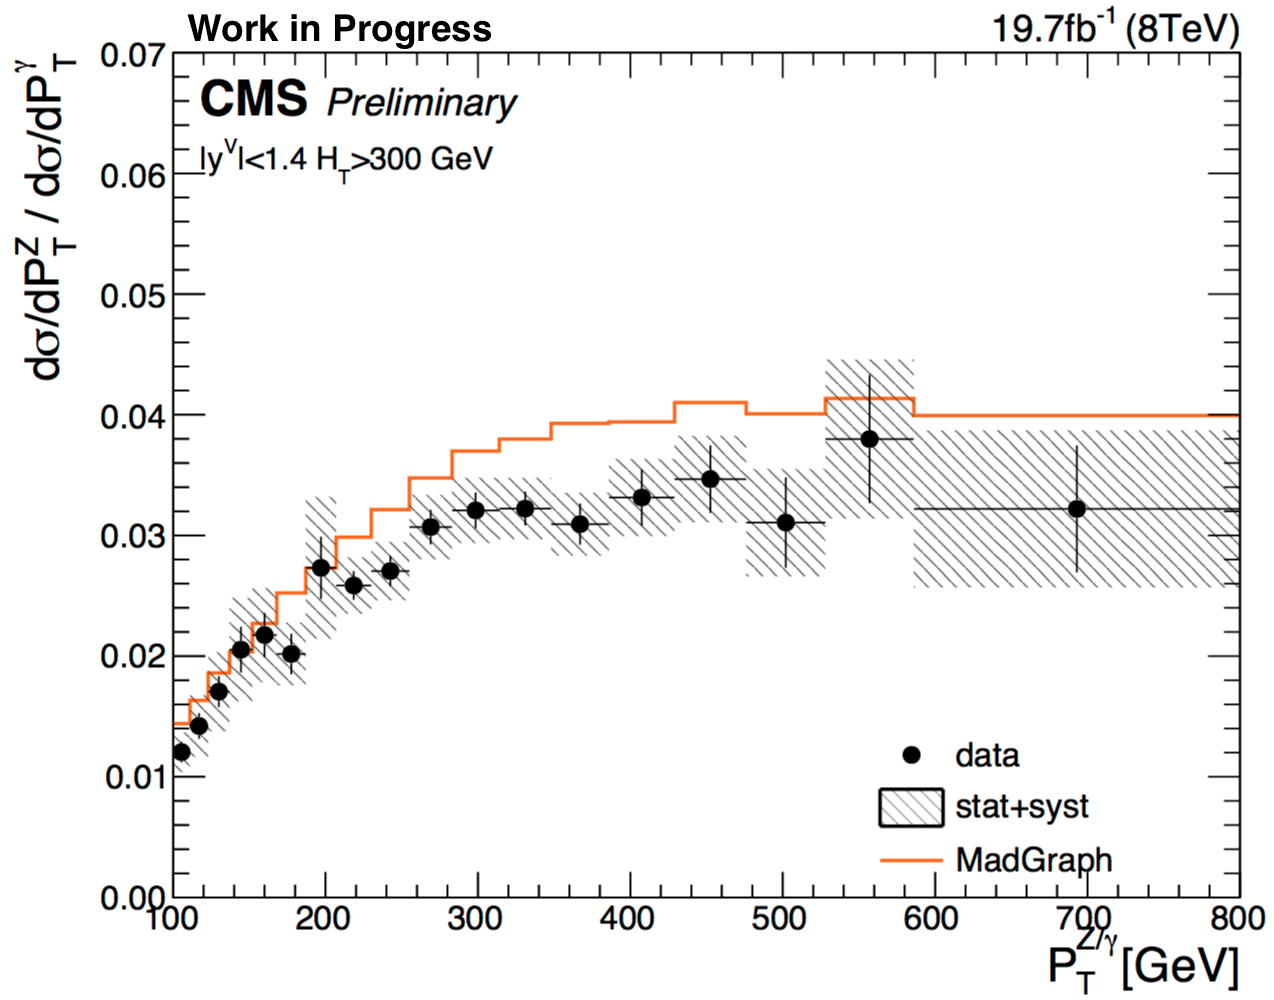
\includegraphics[width=0.6\textwidth]{ZgammaRatio.png}
\end{center}
\vspace{-1em}
\caption[Results of study of the Z+jets to $\gamma+$jets cross-section ratio for both data and MadGraph simulation.]{Results of study of the Z+jets to $\gamma+$jets cross-section ratio for both data and MadGraph simulation. For high values of the vector boson transverse momentum, the ratio between these processes is observed to be nearly constant.}
\label{Zgamma}
\end{figure}

\vspace{1em}

In order to obtain the shape corrections, the ratio between data and simulation of the jet multiplicity distribution is used (\autoref{NjetsCR}). This is due to it exhibiting the highest difference between the observed data and MC. The re-weight for the $\gamma+$jets simulation sample is then accomplished by applying the $N_{jet}$ dependent factor $S_\gamma(N_j)$. This scale factor is determined by taking the ratio of the data and simulation, after subtracting all other MC samples from data events:

\begingroup
	\Large
	\begin{center}
	%\begin{equation}
		$S^{i}_{\gamma} = \frac{\text{Data}^{i} - \text{M}\text{C}^{i}_\text{other}}{\text{M}\text{C}_{\gamma+\text{jets}}^i}$,
	\end{center}
	%\end{equation}
\endgroup

\noindent {where i denotes any given bin in the $N_j$ distribution. The shape correction factors $S^{i}_{\gamma}$ are displayed graphically in \autoref{NjetsCR} (right) for each $N_j$ bin. These factors correct for differences in the jet multiplicity shape, while the overall normalization is estimated from the tight $\mu\mu$ control region. \autoref{NjetsShapeCorr} shows the $N_j$ distribution in the tight $\mu\mu$ control region after the calculated scale factors have been applied. The $S_{\gamma}$ correction will be applied to the Z$\rightarrow\nu\bar{\nu}$ simulation final prediction for each of the analysis search bins. The uncertainty associated with the scale factor is estimated from the event yields in the loose photon control region. This uncertainty will form part of the total systematic uncertainty in the final prediction.}

\begin{figure}[H]
\begin{center}
\begin{minipage}[b]{0.45\textwidth}
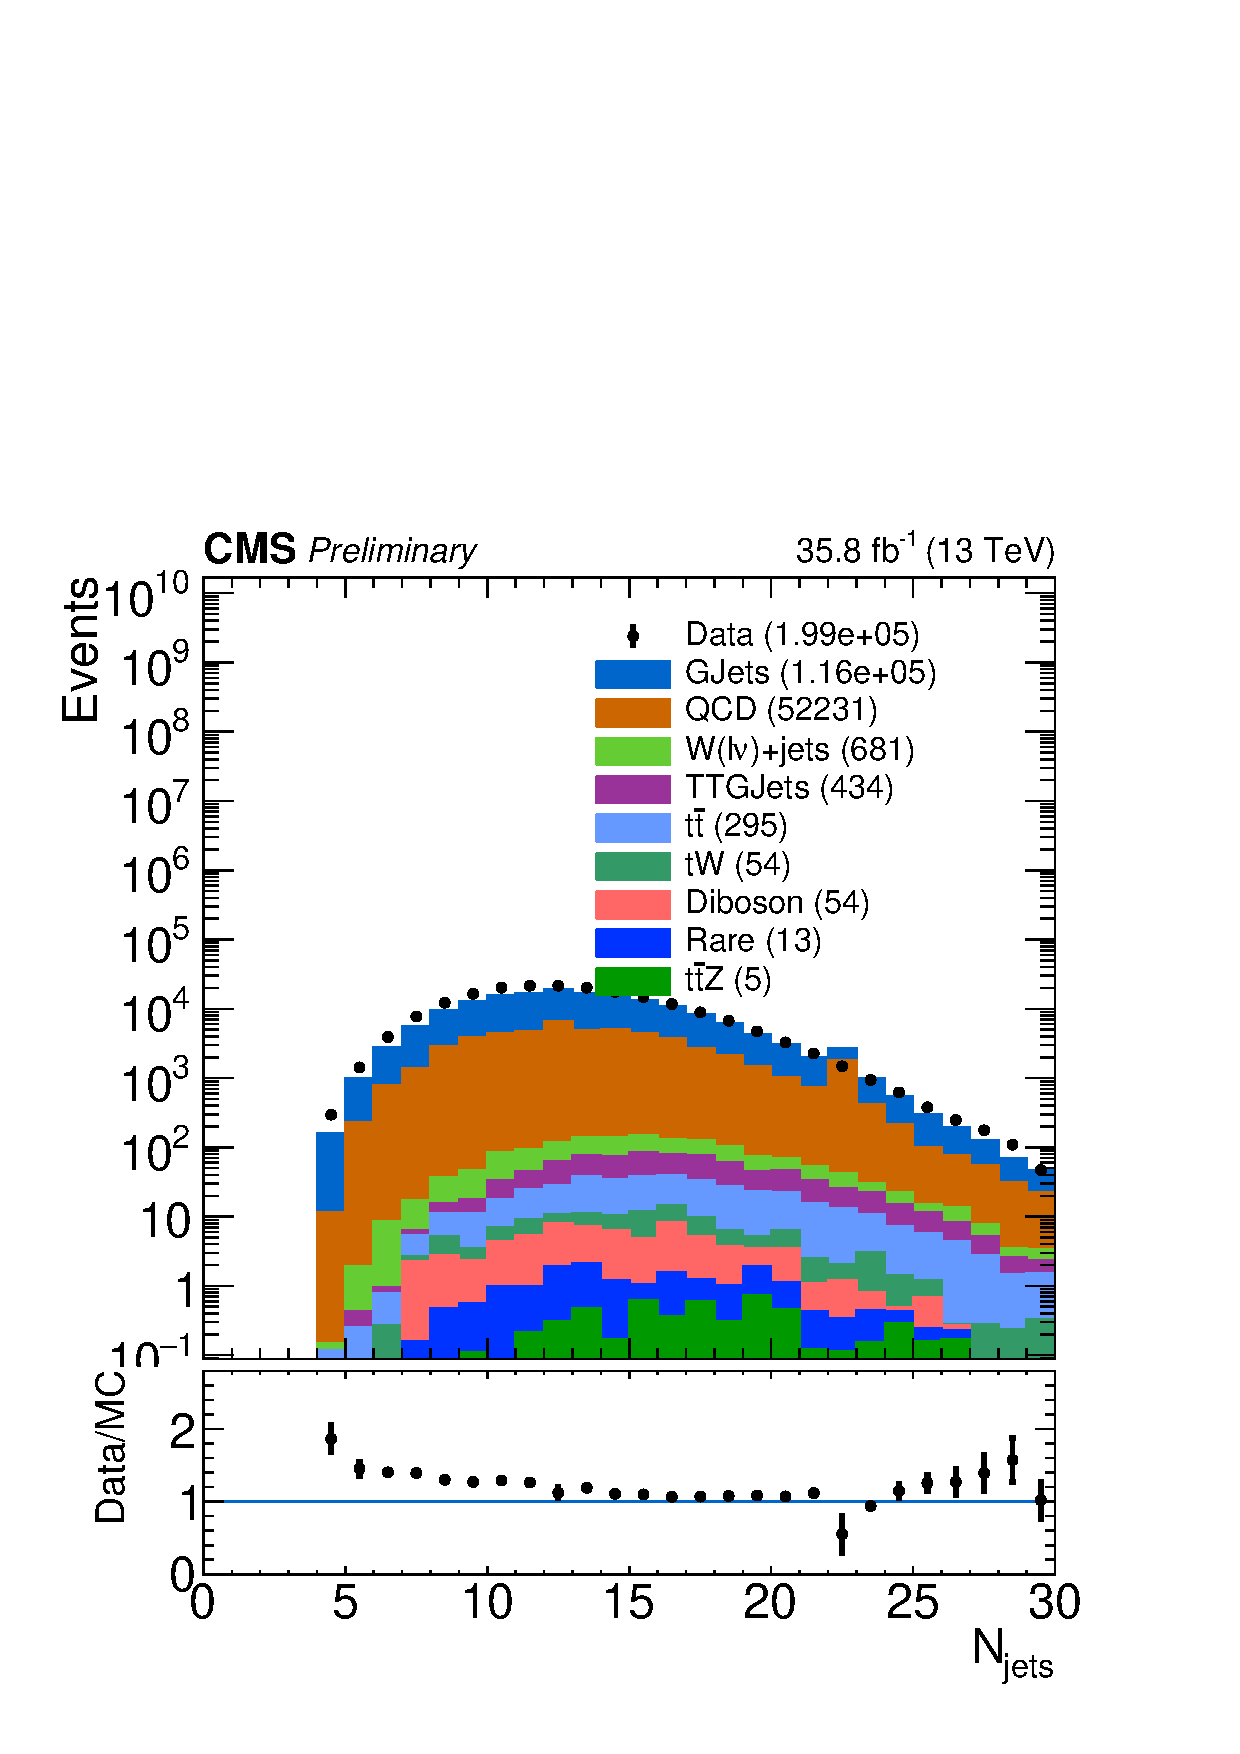
\includegraphics[width=0.94\textwidth]{dataMC_Photon_nj_Log_LooseLepVeto.pdf}
\end{minipage}
\begin{minipage}[b]{0.5\textwidth}
    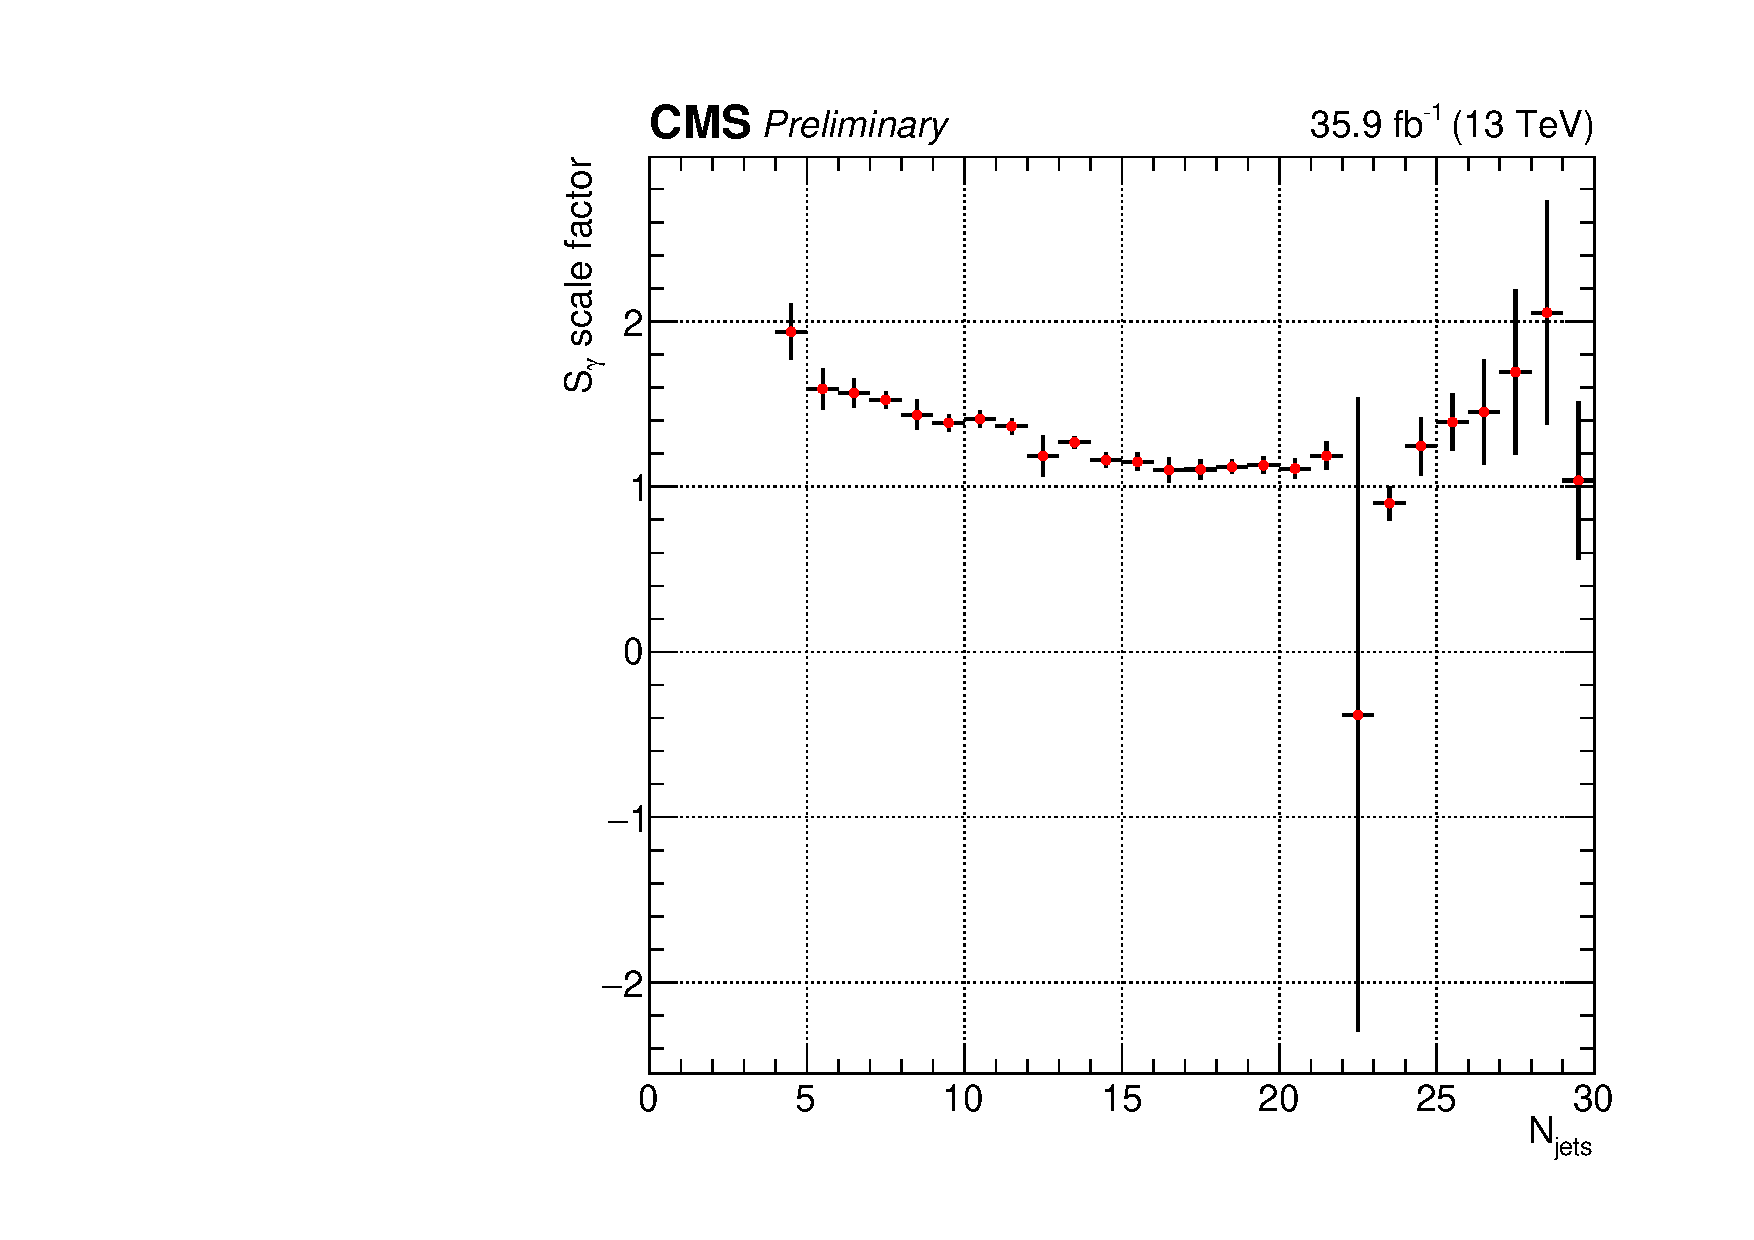
\includegraphics[width=\textwidth]{ShapeCorr_LooseLepVeto.pdf}
\end{minipage}
\end{center}
\vspace{-1em}
\caption{Jet multiplicity and the associated S$_\gamma$ scale factor in the loose photon control region before any corrections are applied.}
\label{NjetsCR}
\end{figure}

%\vspace{1em}

\begin{figure}[H]
\begin{center}
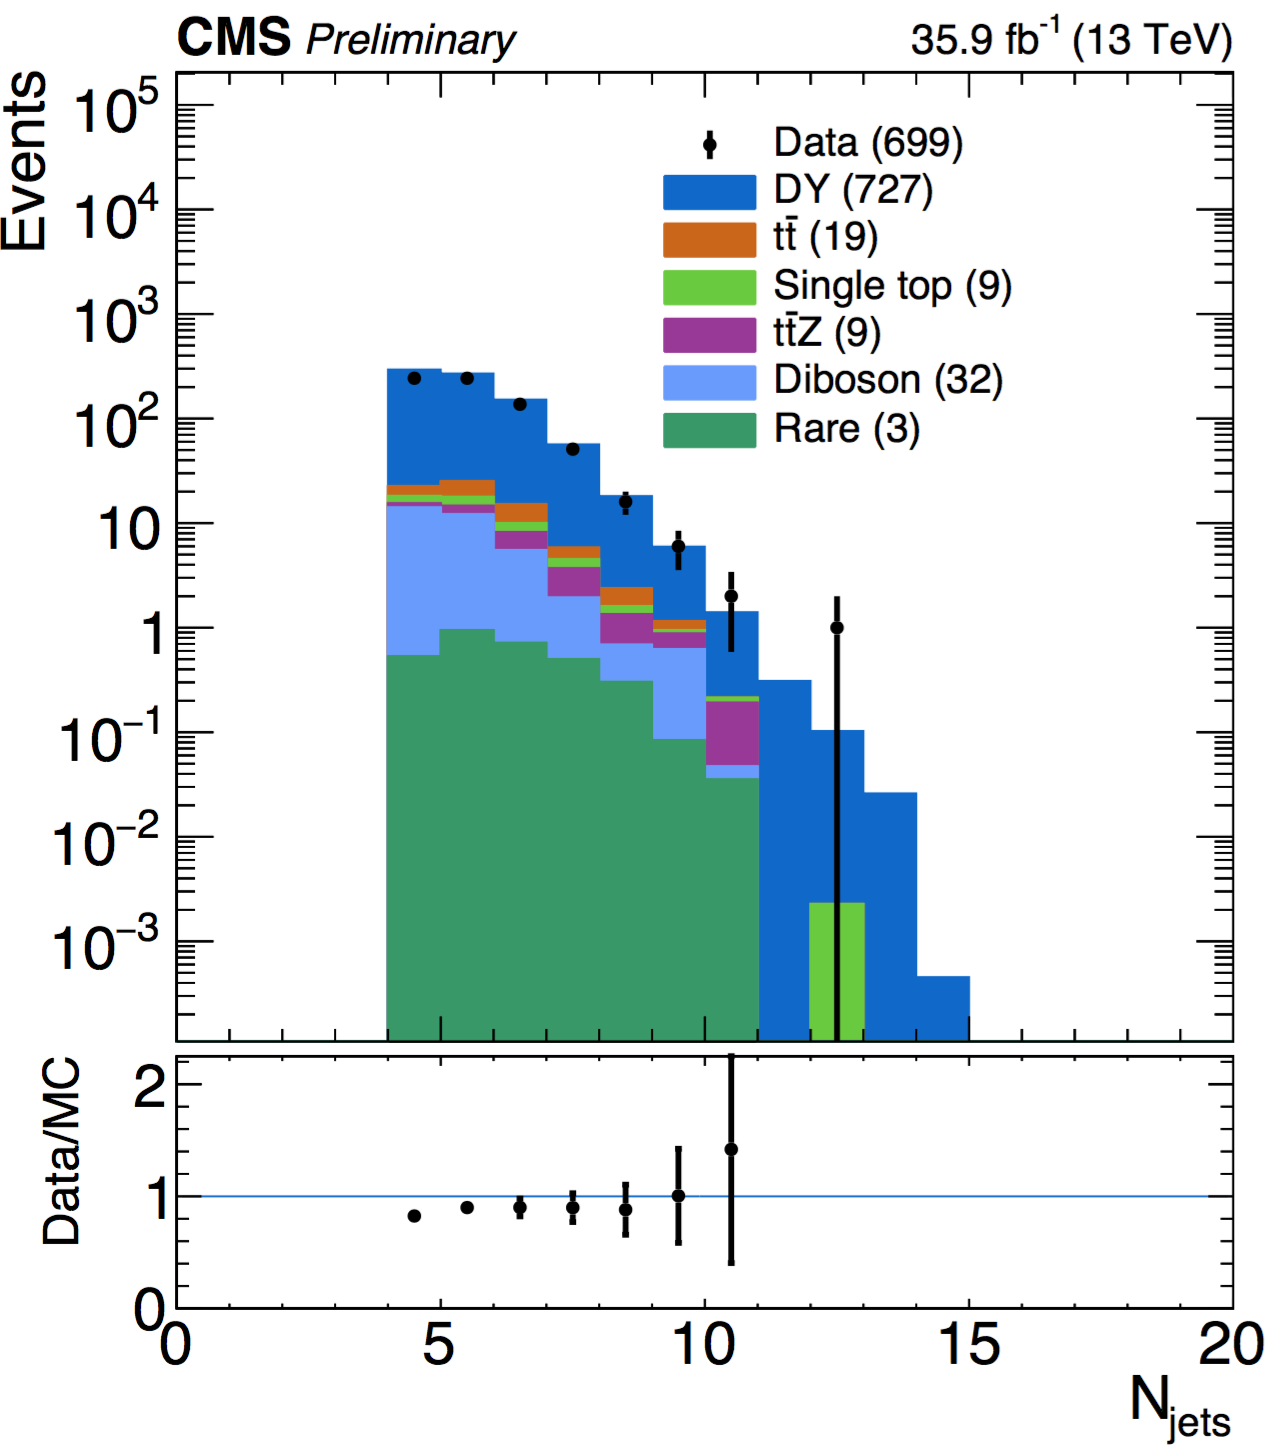
\includegraphics[width=0.4\textwidth]{NjetsShapeCorr.png}
\end{center}
\vspace{-1em}
\caption[$N_{jet}$ distribution in the tight $\mu\mu$ control region after $S_\gamma$ corrections.]{$N_{jet}$ distribution in the tight $\mu\mu$ control region after $S_\gamma$ corrections.}
\label{NjetsShapeCorr}
\end{figure}

The effect of the $S_{\gamma}$($N_j$) scale factor is shown for various distributions. These results show that the overall agreement between data and simulation improves after applying the corresponding shape corrections.

\begin{figure}[H]
\begin{center}
\begin{minipage}[b]{0.45\textwidth}
    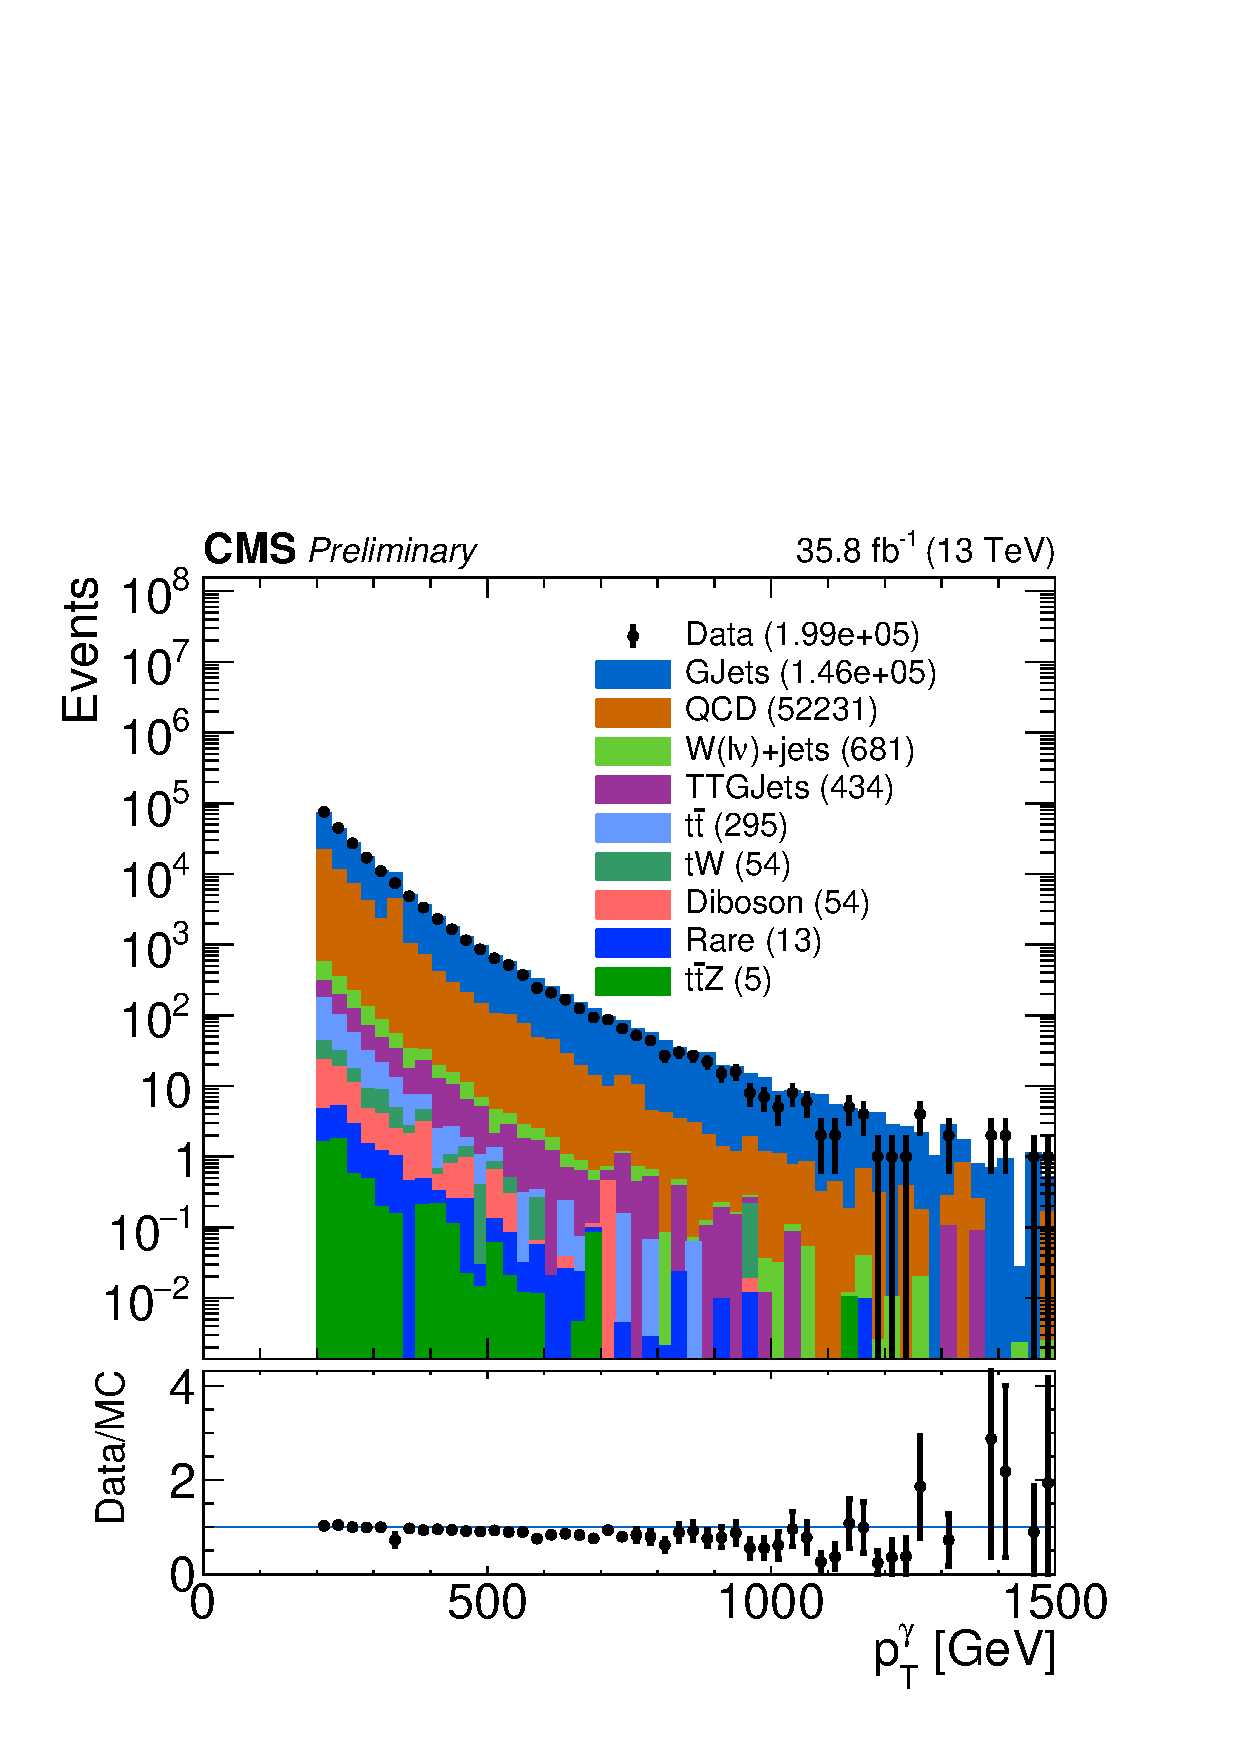
\includegraphics[width=\textwidth]{dataMC_PhotonPt_Wgt_LooseLepVeto.pdf}
\end{minipage}
\begin{minipage}[b]{0.45\textwidth}
    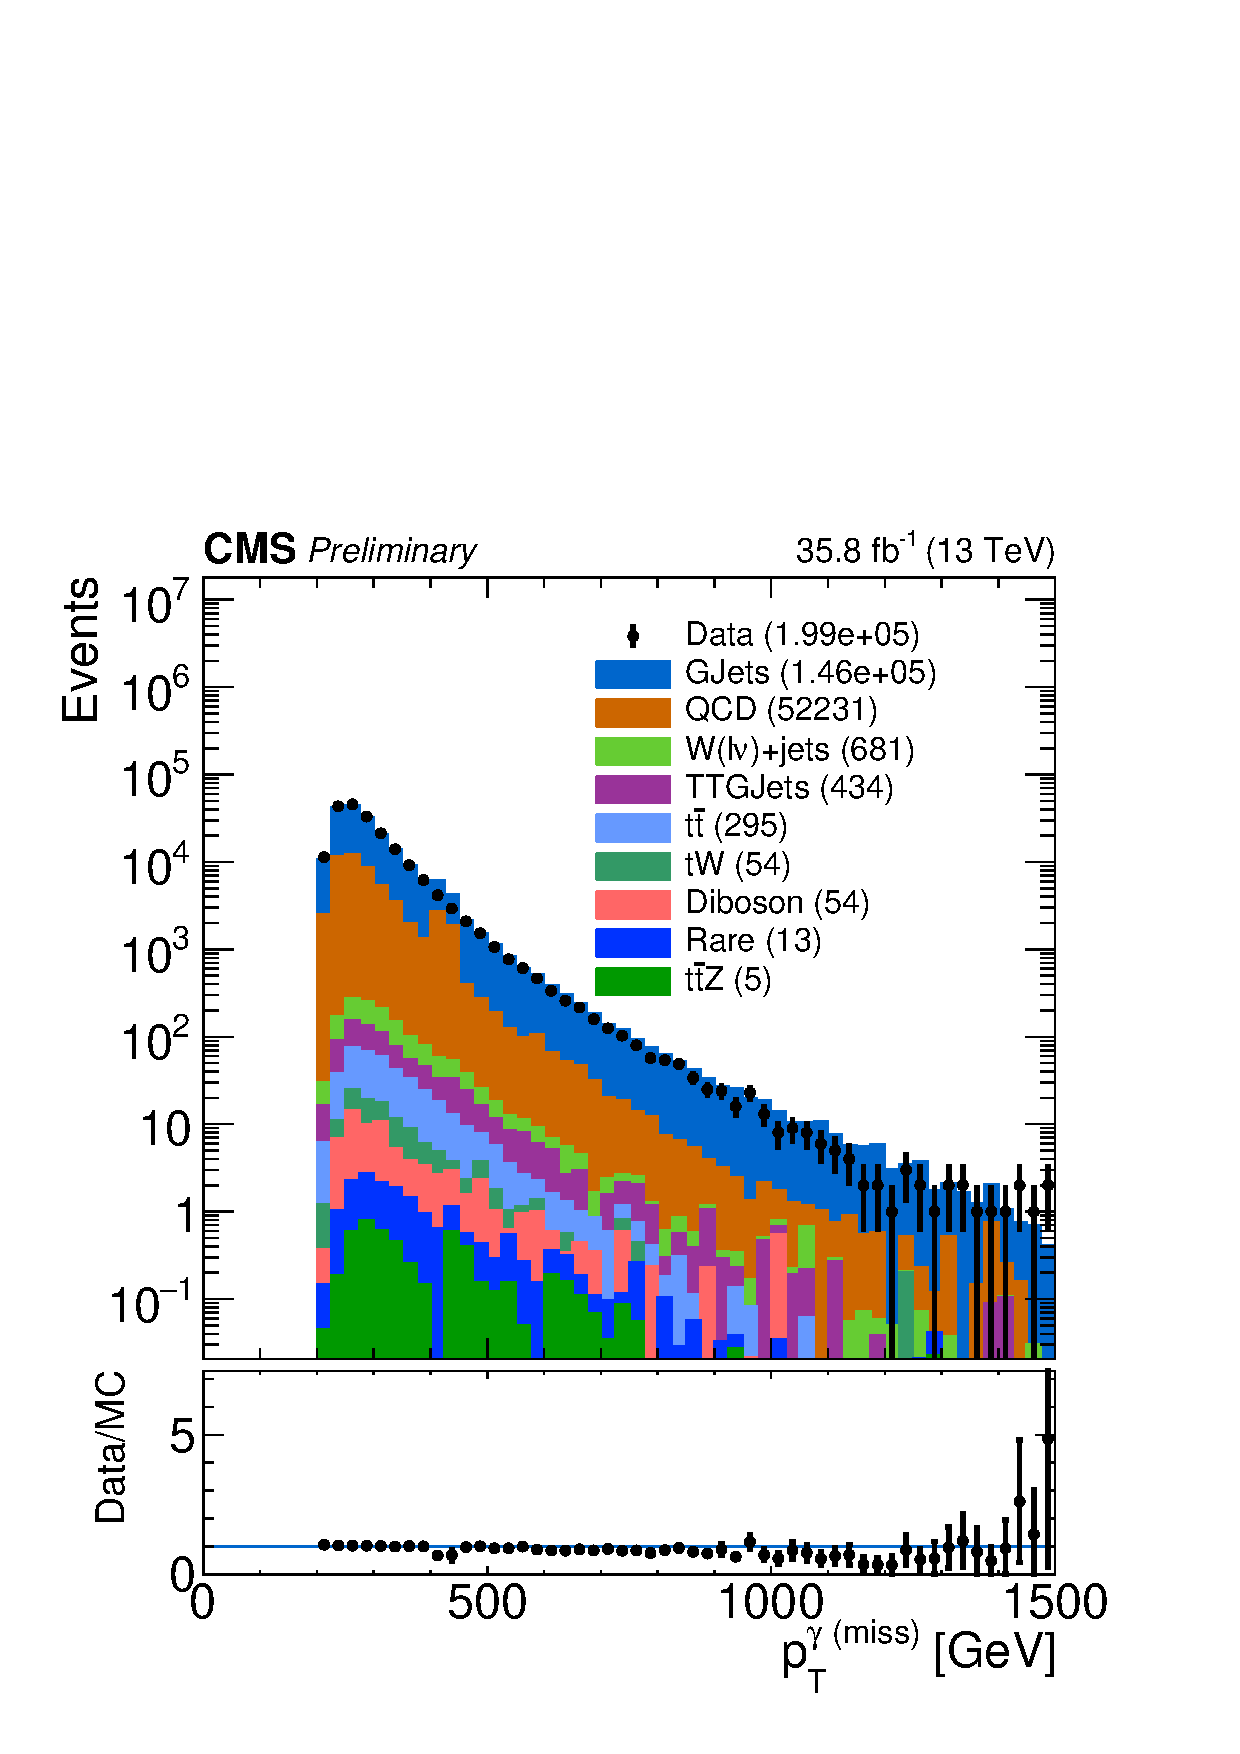
\includegraphics[width=\textwidth]{dataMC_MetGamma_Wgt_LooseLepVeto.pdf}
\end{minipage}
\end{center}
\vspace{-1em}
\caption{$p_\text{T}^\gamma$ (left) and $p_\text{T}^{\gamma (miss)}$ (right) distributions after applying the $S_\gamma$($N_j$) scale factor. Comparing to \autoref{PtMetPt}, an improvement in the agreement between data/MC can be observed.}
\label{PtMetPtCorr}
\end{figure}

\vspace {1em}

\begin{figure}[H]
\begin{center}
\begin{minipage}[b]{0.45\textwidth}
    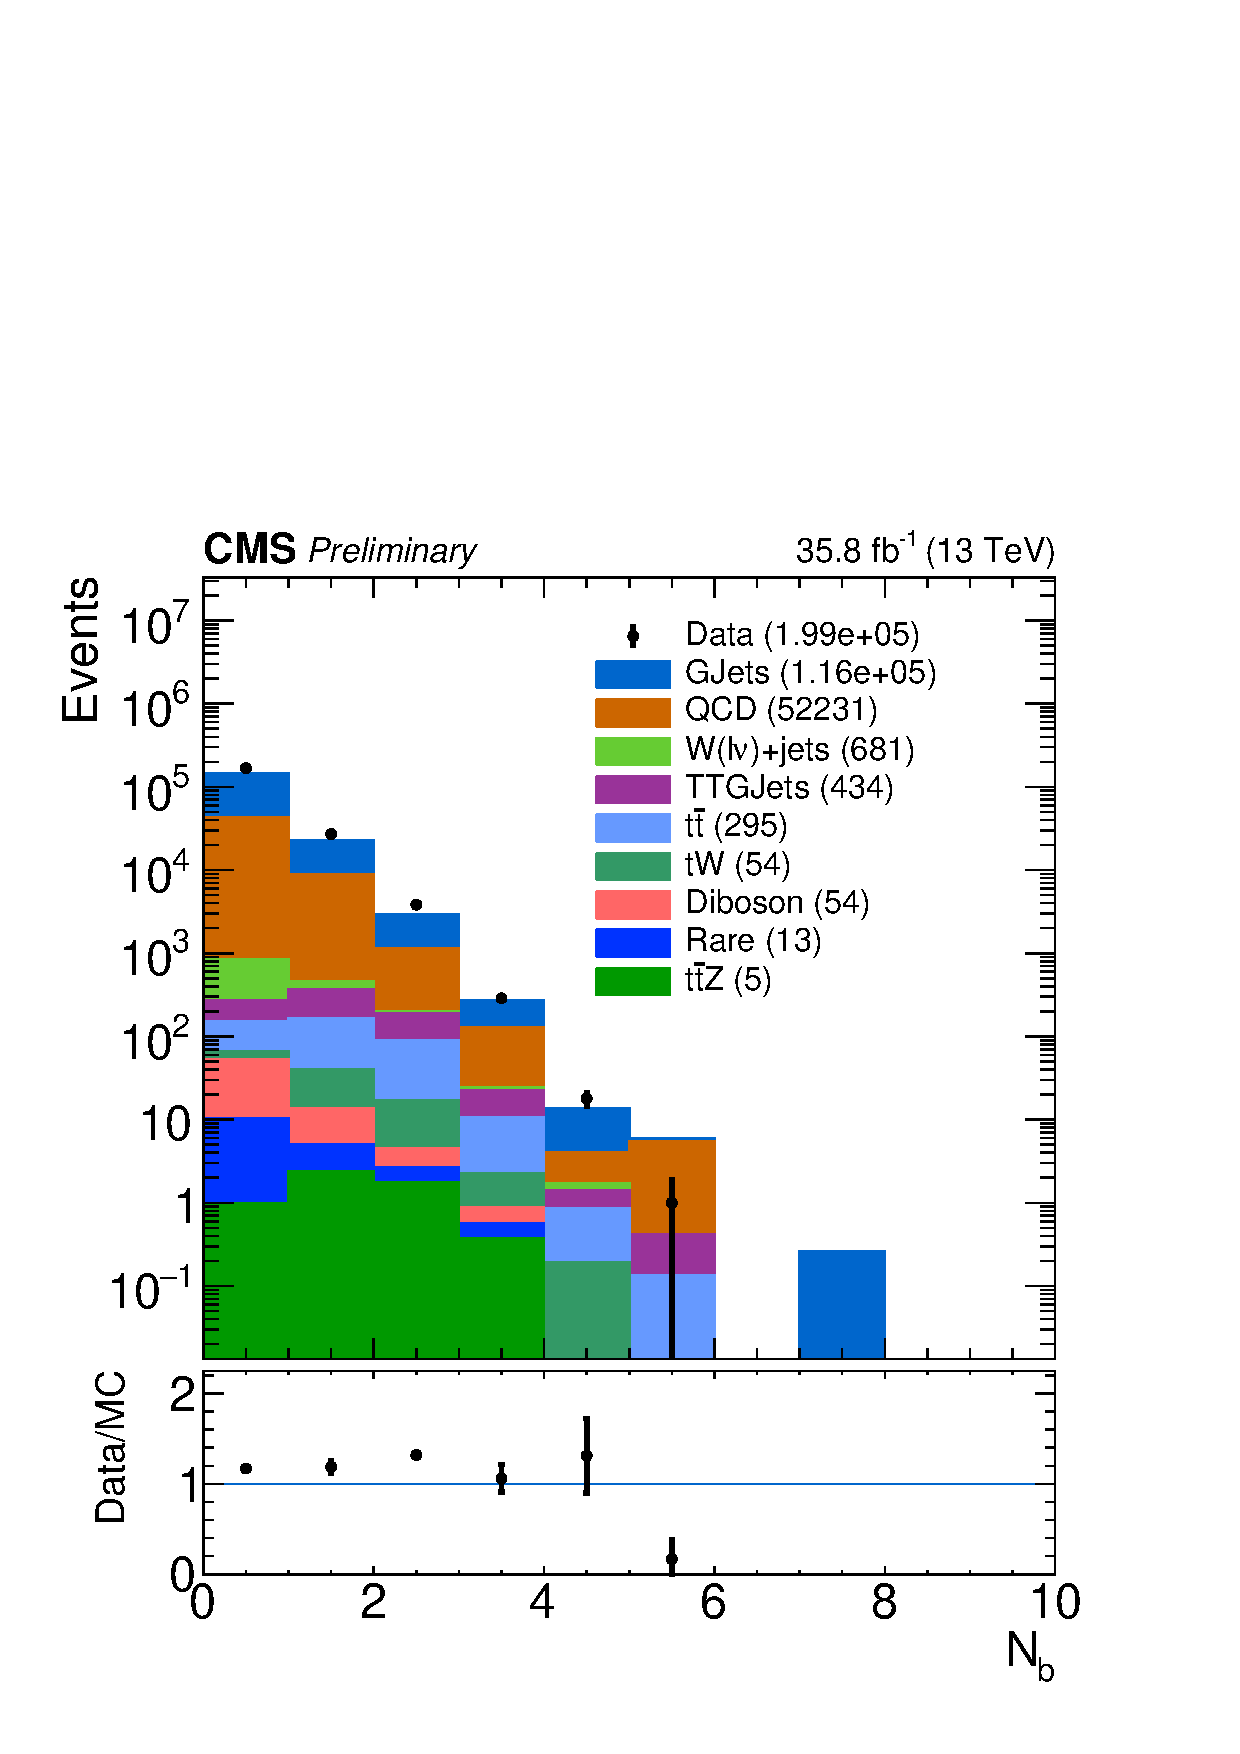
\includegraphics[width=\textwidth]{dataMC_Photon_nb_Log_LooseLepVeto.pdf}
\end{minipage}
\begin{minipage}[b]{0.45\textwidth}
    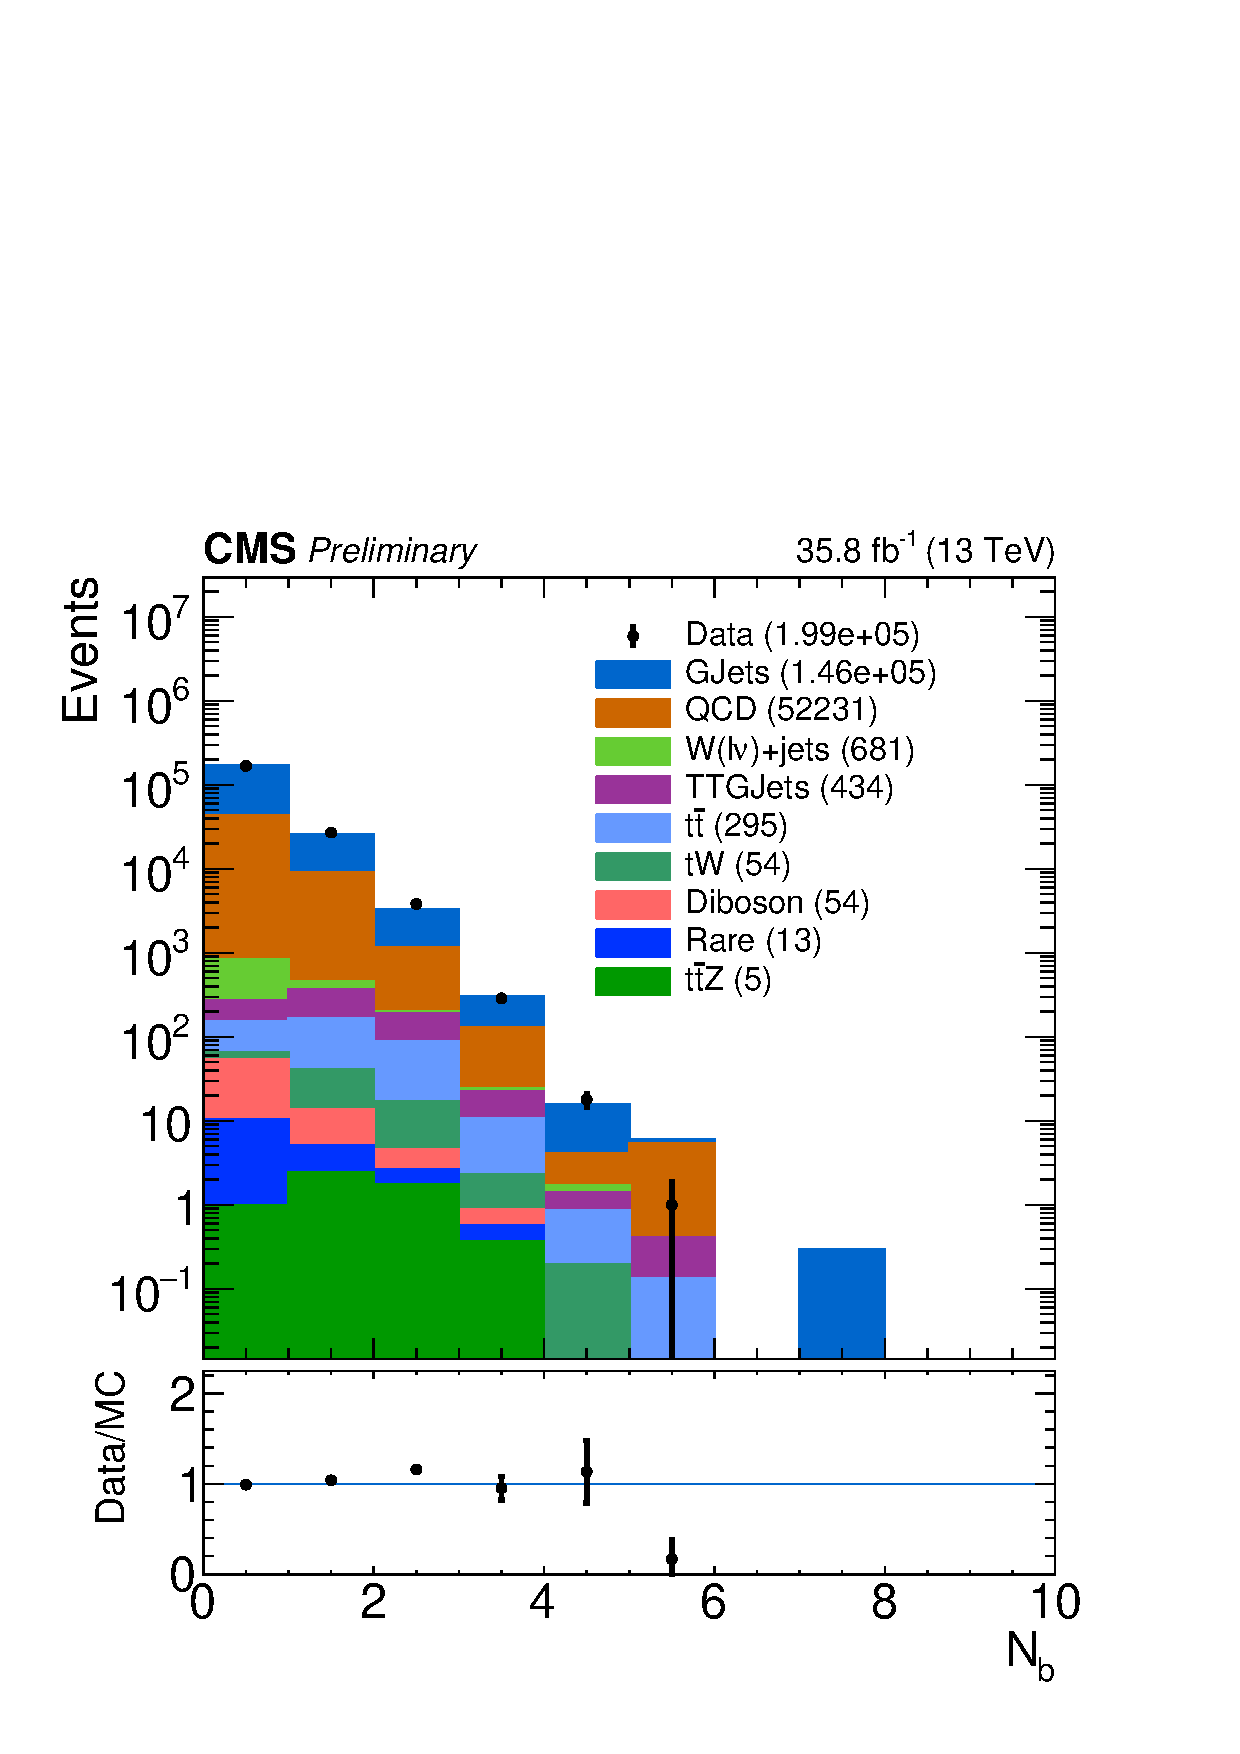
\includegraphics[width=\textwidth]{dataMC_Photon_nb_Log_Wgt_LooseLepVeto.pdf}
\end{minipage}
\end{center}
\vspace{-1em}
\caption{$N_b$ distribution before (left) and after (right) applying the $S_\gamma$($N_j$) scale factor. }
\end{figure}

%\vspace {1em}

\begin{figure}[tb]
\begin{center}
\begin{minipage}[b]{0.45\textwidth}
    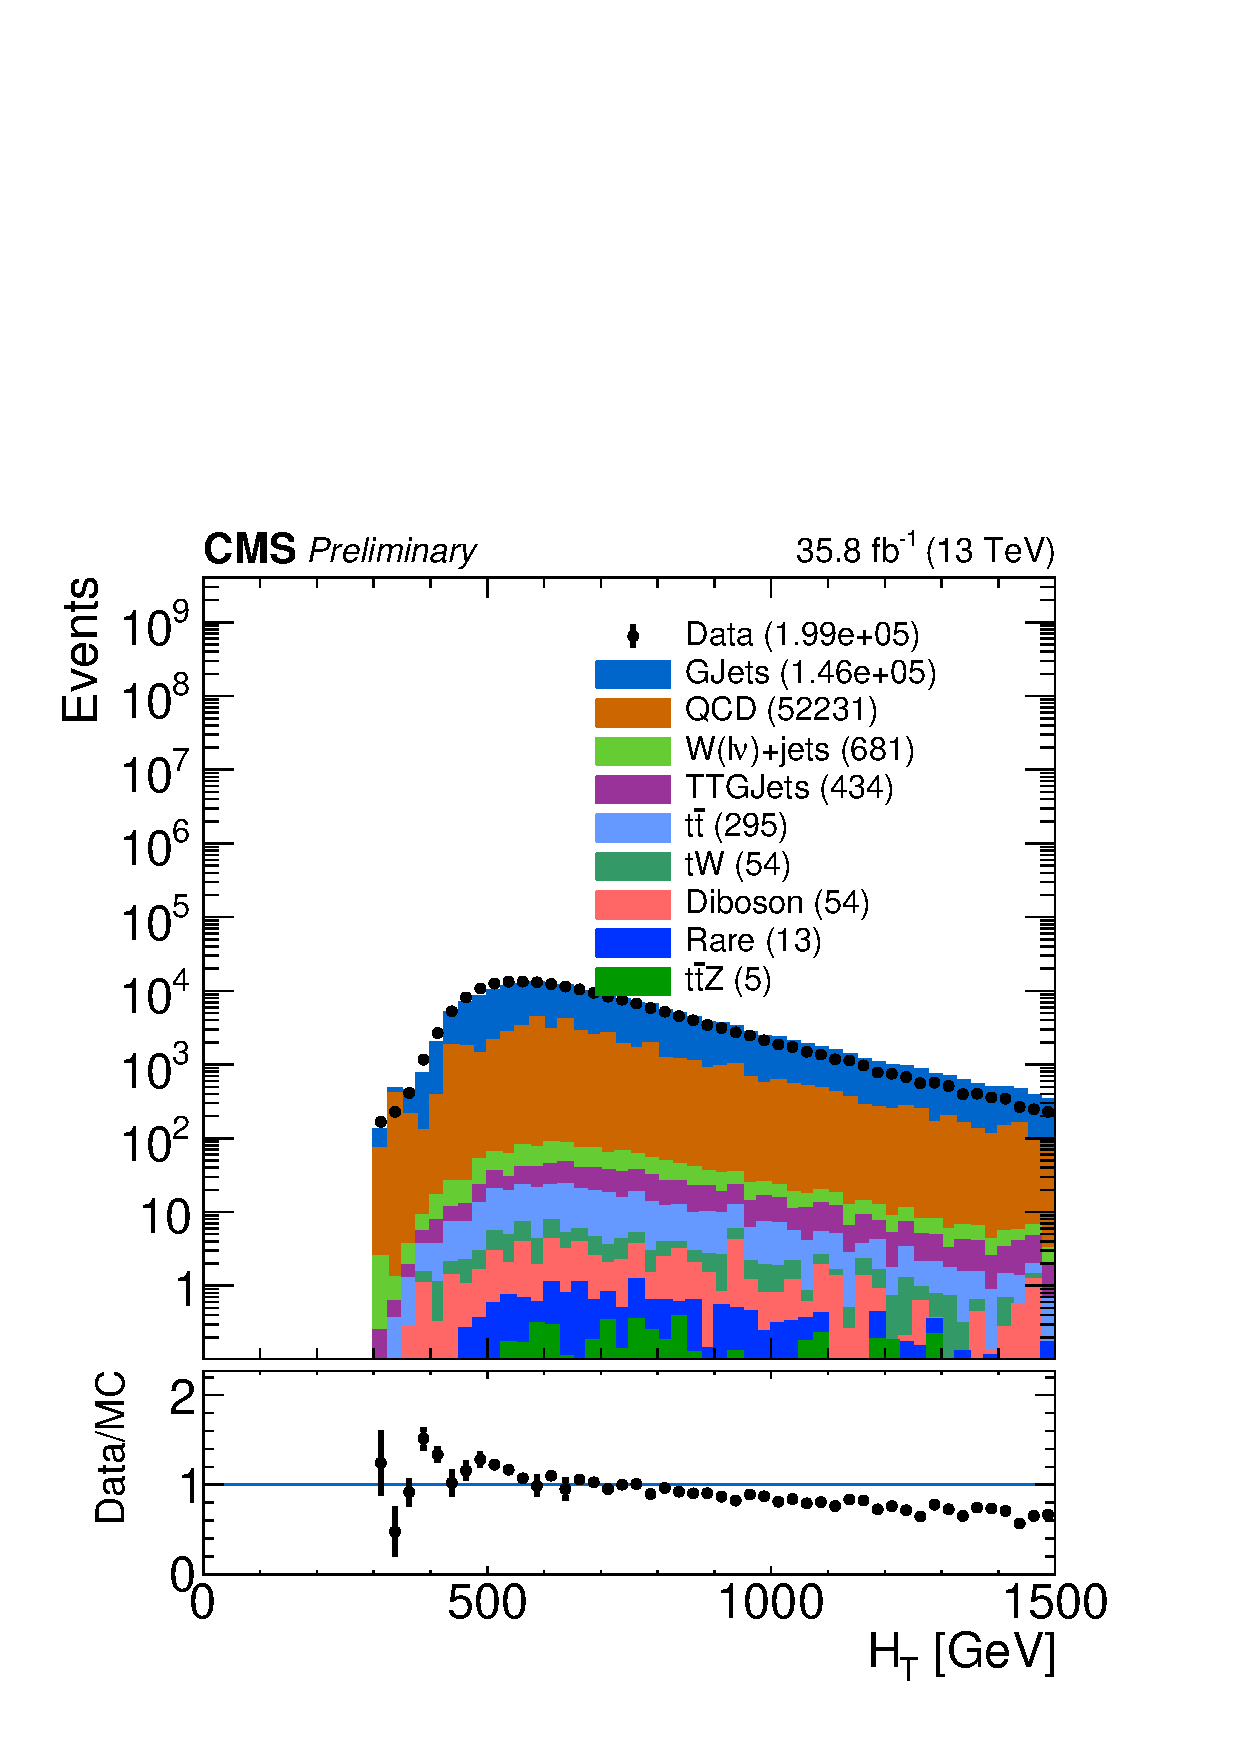
\includegraphics[width=\textwidth]{dataMC_Photon_ht_Wgt_LooseLepVeto.pdf}
\end{minipage}
\begin{minipage}[b]{0.45\textwidth}
    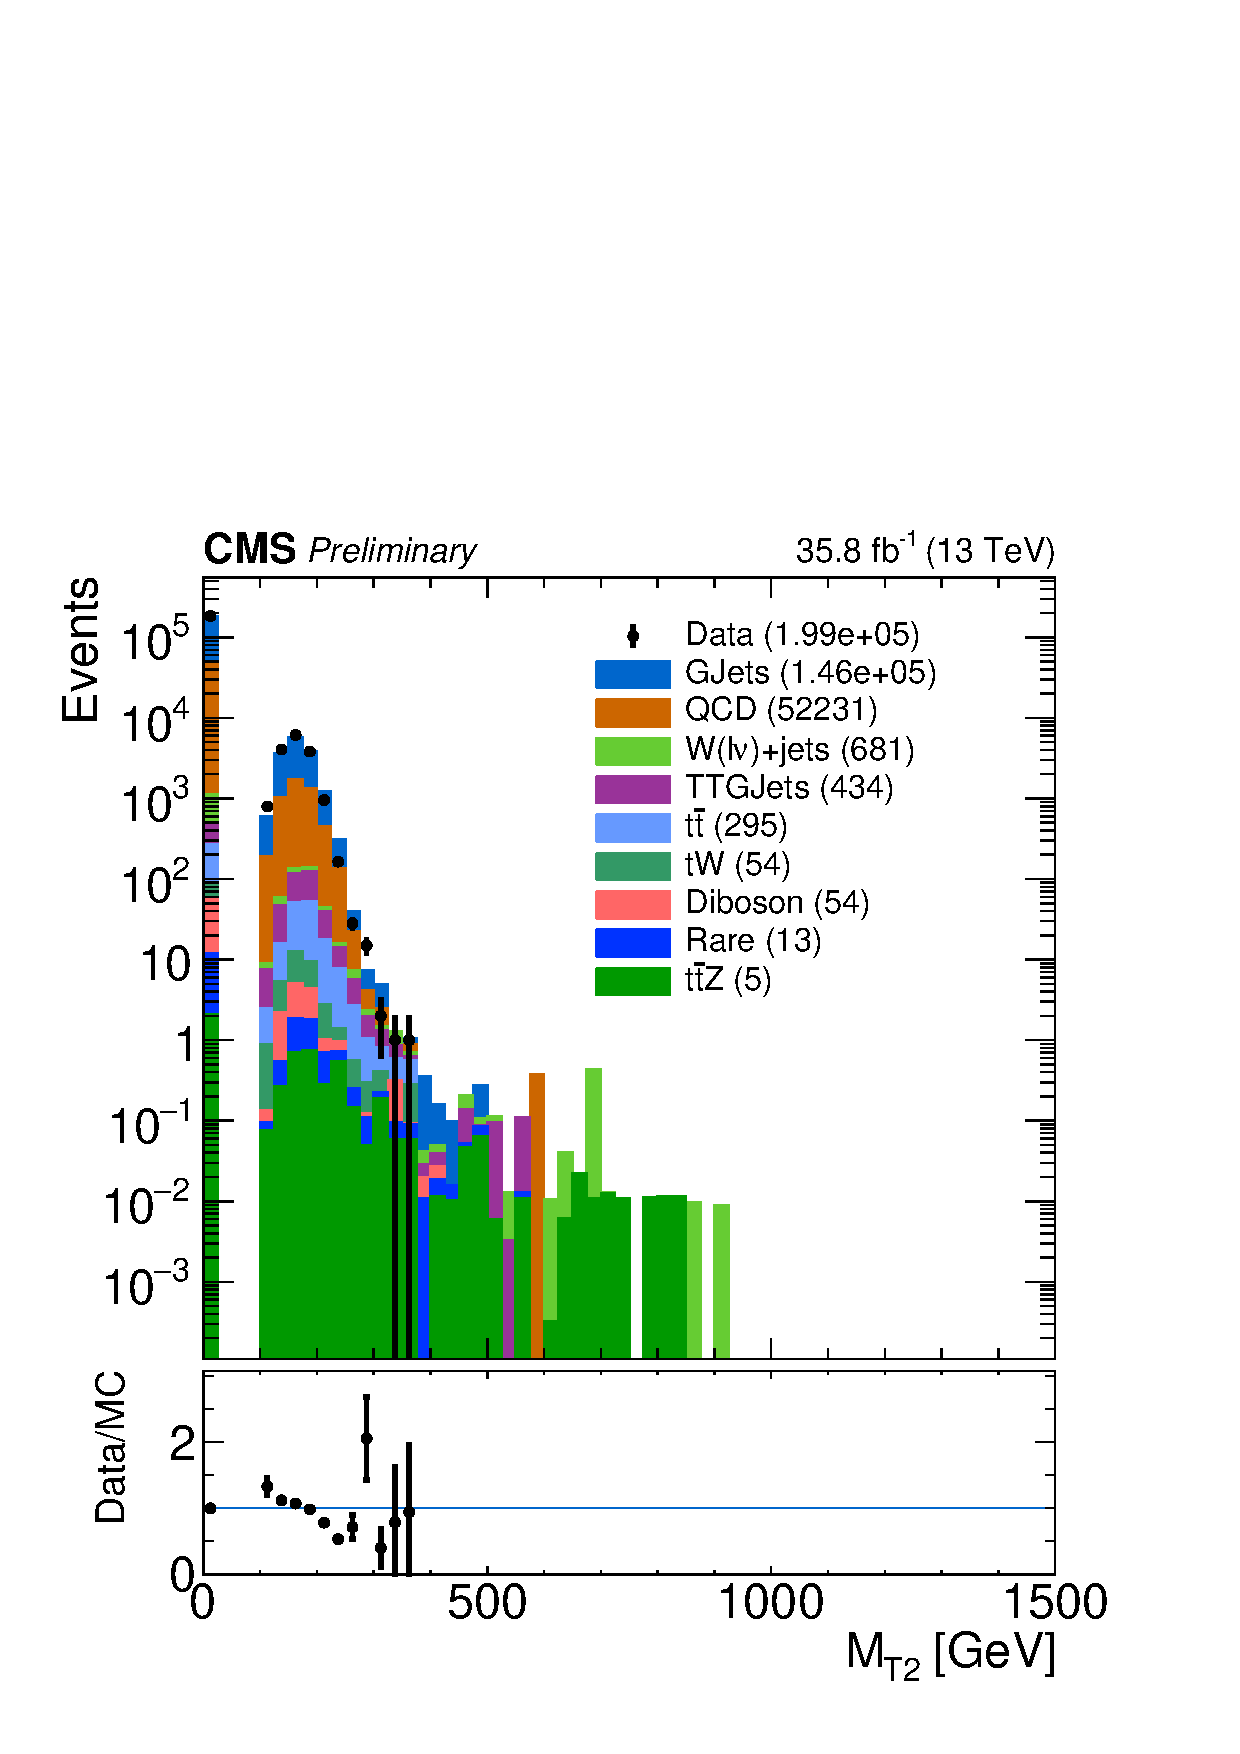
\includegraphics[width=\textwidth]{dataMC_Photon_mt2_Wgt_LooseLepVeto.pdf}
\end{minipage}
\end{center}
\vspace{-1em}
\caption{$H_\text{T}$ and $m_\text{T2}$ distributions applying the $S_\gamma$($N_j$) scale factor. }
\end{figure}

\subsection{Normalization Correction Using the tight Z$\rightarrow\mu^{+}\mu^{-}$ Control Sample}\label{tightmumu}

In order to constrain the normalization of the Z$\rightarrow\nu\bar{\nu}$ simulation sample, a normalization correction factor $R_{norm}$ is calculated from the tight $\mu\mu$ control region defined in \autoref{tightmumu}. Two categories are considered: the zero b-tagged jet category ($N_b = 0$), and the $\geq 1$ b-tagged jet category ($N_b \geq 1$). Both of these categories are statistically consistent with each other but the inclusive region ($N_b \geq 0$) has a lower overall uncertainty. The method used to calculate the normalization scale factor requires that the $N_j$-dependent shape correction factors already be applied. Then, the $R_{norm}$ factor can be extracted from the ratio of the total event yield in data to that in the simulation. This factor is found to be:

\begingroup
	\begin{center}
		$R_{norm} = 1.070 \pm 0.085$,
	\end{center}
\endgroup

\noindent where the uncertainty includes only the associated statistical uncertainties on data and simulation. This uncertainty is found to be propagated to the final background prediction, see \autoref{systematics}.\\

\begin{figure}[H]
\begin{center}
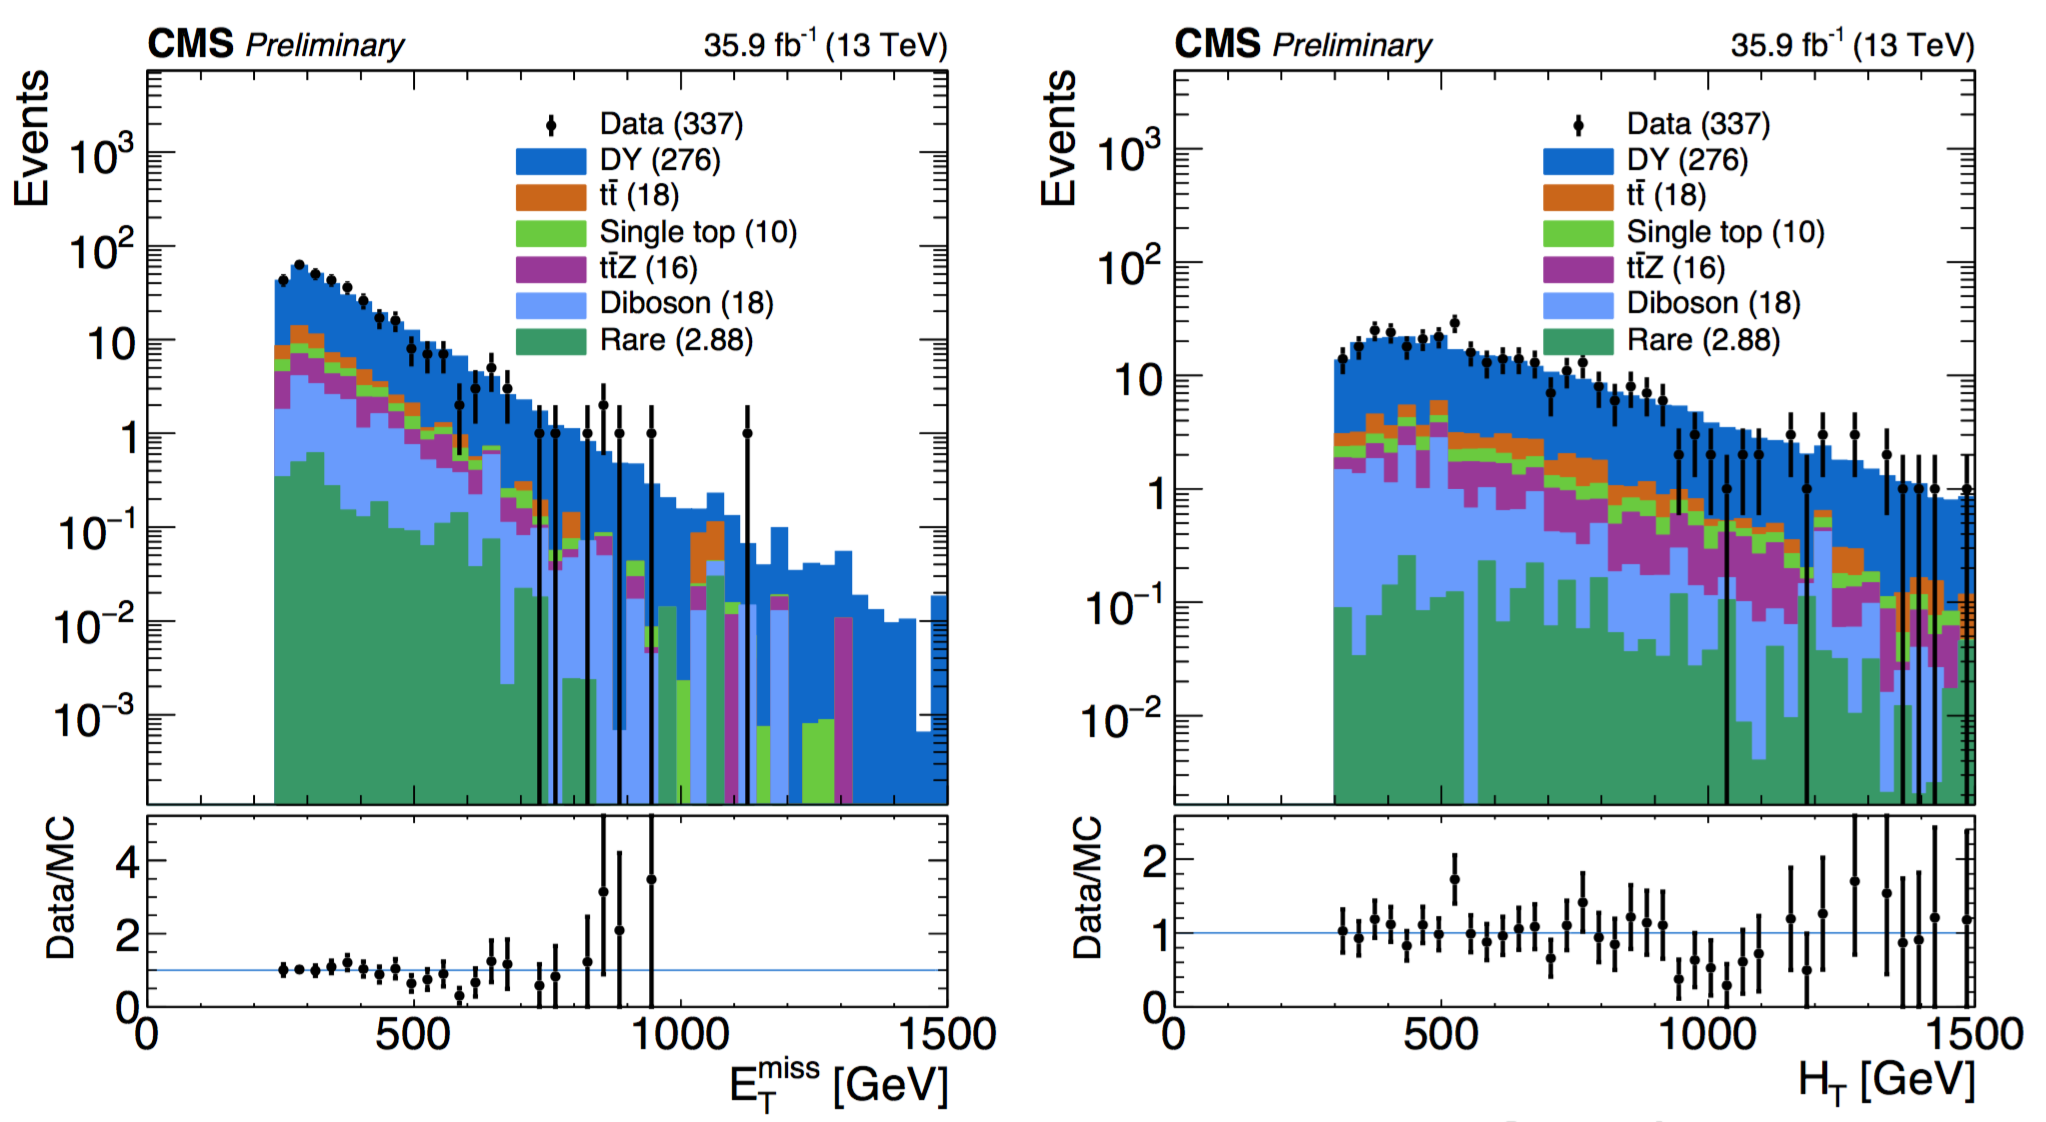
\includegraphics[width=\textwidth]{Rnorm1}
\end{center}
\vspace{-1em}
\caption{Shown are data/MC comparisons for the $p_\text{T}^{miss}$ (left) and $H_\text{T}$ (right) distributions after applying both the $N_j$-dependent shape corrections ($S_\gamma$) and the global normalization scale factor ($R_{norm}$).}
\label{Rnorm1}
\end{figure}

\vspace{1em}

Data/MC comparisons are shown in \autoref{Rnorm1} and \autoref{Rnorm2} after applying $R_{norm}$ for several distributions in the study. With this final global scale factor all the required ingredients for the central value of the Z$\rightarrow\nu\bar{\nu}$ background prediction are obtained. 

\begin{figure}[H]
\begin{center}
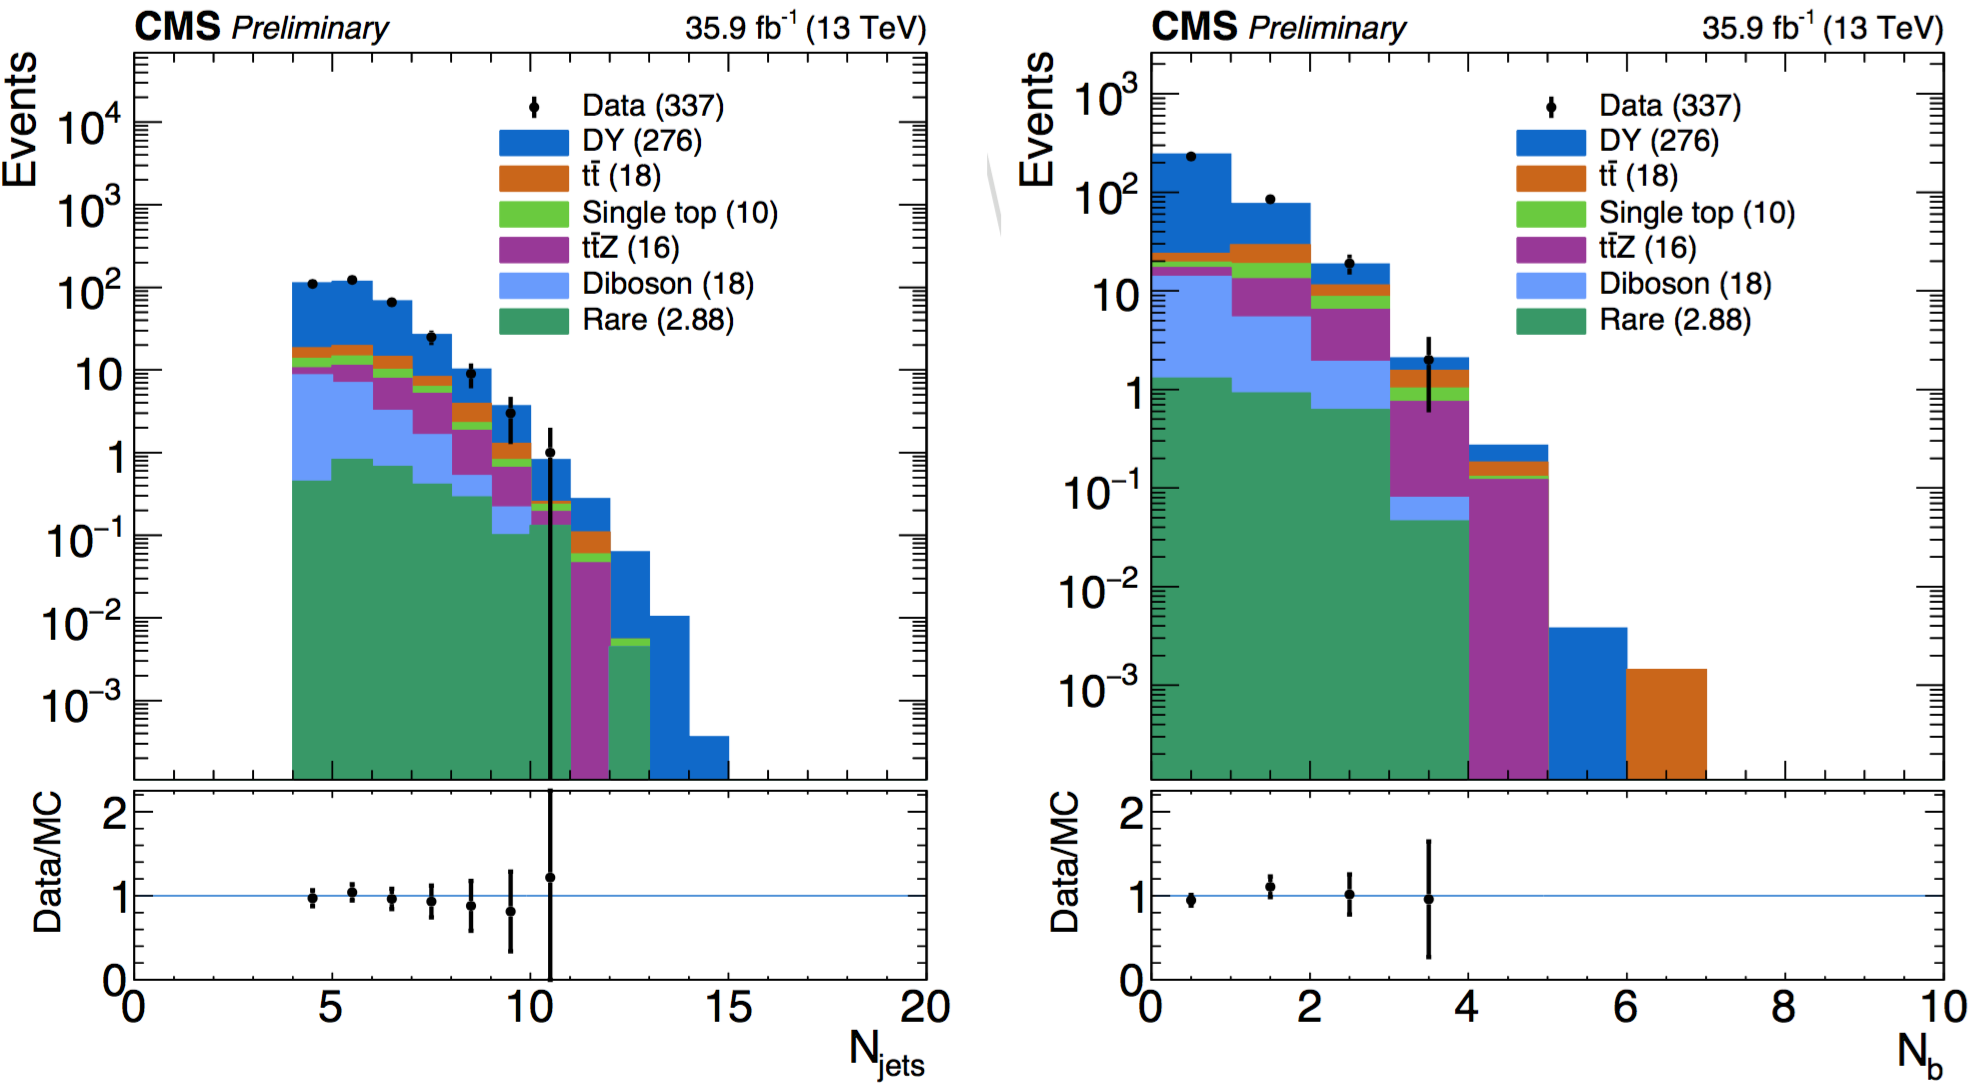
\includegraphics[width=\textwidth]{Rnorm2}
\end{center}
\vspace{-1em}
\caption{Shown are data/MC comparisons for the $N_j$ (left) and $N_b$ (right) distributions after applying both the $N_j$-dependent shape corrections ($S_\gamma$) and the global normalization scale factor ($R_{norm}$).}
\label{Rnorm2}
\end{figure}

\section{Results}

In this section the results for the final estimation of the of the Z$\rightarrow\nu\bar{\nu}$ are presented. The current study includes preliminary results using only data obtained at the CMS detector during 2016. The results for this study are intended to confirm the assumption that the additional $\gamma+$jets control region introduced in this analysis reduce the overall uncertainties obtained in the 2016 analyses (described in \autoref{AnalysisChap}). Furthermore, this study is intended as a benchmark for future analyses of the SUSY stop group based in Fermilab and will be the method used for the 2017 CMS data.

\subsection{Systematics}\label{systematics}

Two categories of uncertainties for the Z$\rightarrow\nu\bar{\nu}$ prediction are considered: uncertainties that are associated to the use of MC simulation and the uncertainties specifically associated to the background prediction method. Several sources are acknowledged in the first category mentioned such as PDF and renormalization/factorization scale choices, jet and $p_\text{T}^{miss}$ energy scale uncertainties b-tag scale factor uncertainties, and trigger efficiency uncertainties. Given that the simulation sample is normalized to data in the tight control region, uncertainties associated with the luminosity and cross-section are excluded. In addition, the overall Z$\rightarrow\nu\bar{\nu}$ statistical uncertainty from MC simulation is also taken into account.\\

\begin{figure}[H]
\begin{center}
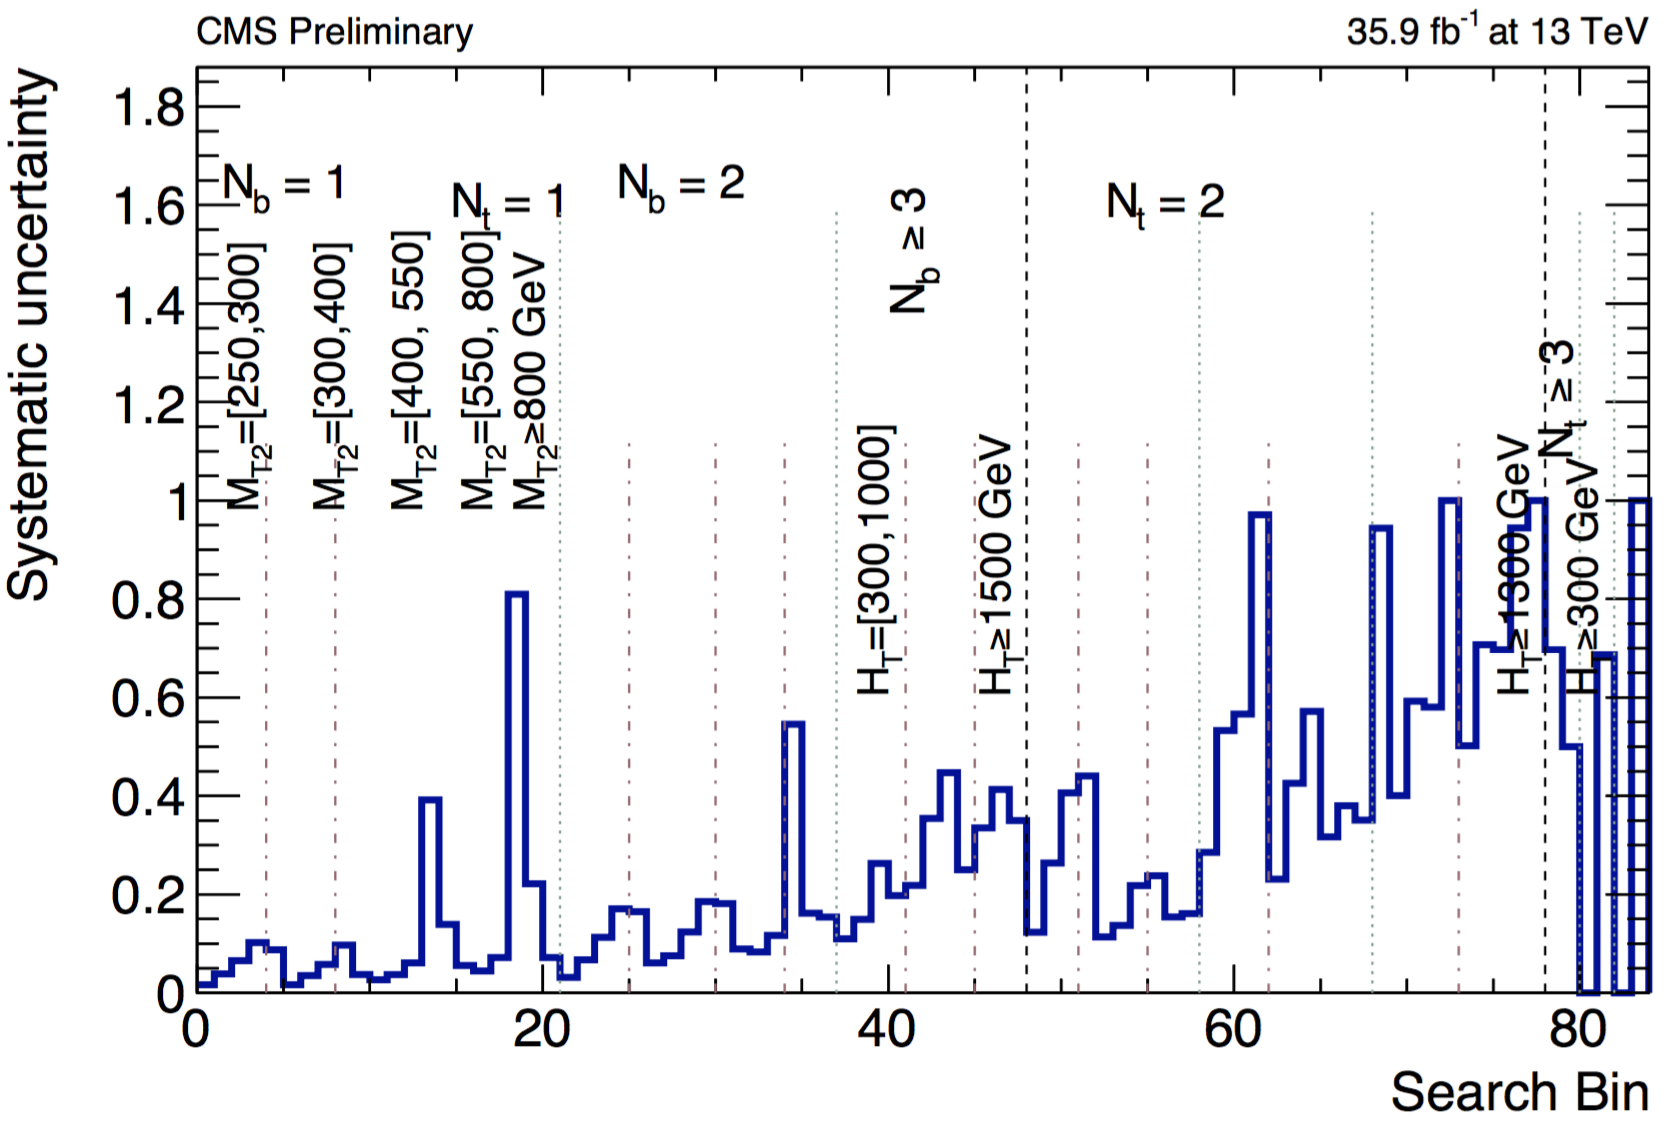
\includegraphics[width=0.8\textwidth]{UncZnunu}
\end{center}
\vspace{-1em}
\caption{Systematic uncertainty in the final prediction, as a function of the search bin, associated to the MC statistics.}
\label{UncZnunu}
\end{figure}

The statistical uncertainty associated with each bin in the MC is propagated as a systematic uncertainty. The relative uncertainty per bin can be see in \autoref{UncZnunu}. It shows that the uncertainties for the MC vary from as low as 1\% up to 81\% and even 100\% in some regions. Since the final estimation is scaled using the global normalization factor from the tight $\mu\mu$ control region ($R_{norm}$), the total uncertainty, due to limited amounts of events in data, is propagated in the final prediction. This is also true for the $S_\gamma$($N_j$) scale factor, in which the residual differences in search variables other than $N_j$ are evaluated in the loose photon control region. Both the uncertainty arising from the $N_j$ re-weighting as well as the residual differences are evaluated together. The uncertainty from $R_{norm}$ is propagated as a flat value of 7.9\% uncertainty per each search bin.

\subsection{Z$\rightarrow\nu\bar{\nu}$ Estimation for the Search Bins}

The final estimation for the Z$\rightarrow\nu\bar{\nu}$ background calculated for all 84 search bins is shown in \autoref{results}. The statistical uncertainty in bins that have zero events is treated as the average weight (the sum of the weights squared over the weight) times the poisson error on 0 which is 1.8. This average weight is calculated on the basis of a relaxed cut in which $N_b \geq 2$ is required. For comparison, a cut in which $N_t > 2$ where two tops are fake for the Z$\rightarrow\nu\bar{\nu}$ is used.

\begin{figure}[H]
\begin{center}
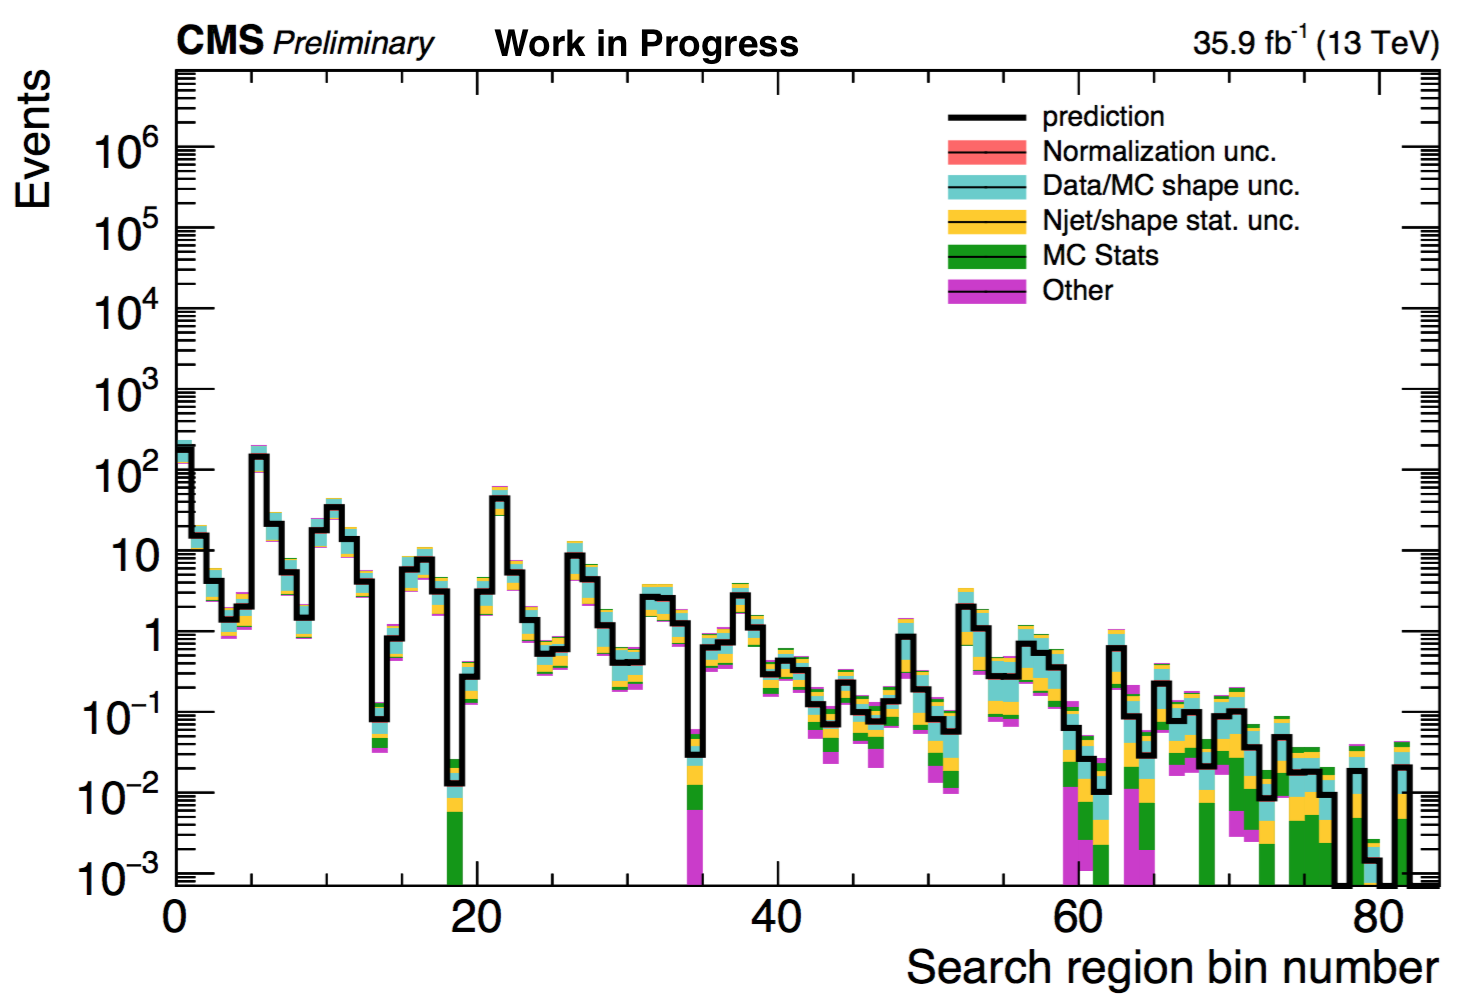
\includegraphics[width=0.8\textwidth]{Results.png}
\end{center}
\vspace{-1em}
\caption{Z$\rightarrow\nu\bar{\nu}$ background prediction for all search bins, including the breakdown of the various uncertainties.}
\label{results}
\end{figure}



%\chapter{Conclusion}\label{conclusion}
%\input{chapters/conclusion}


%\appendix
%\chapter{Appendix Title}
%%\input{chapters/appendix}

\bibliography{references}
\bibliographystyle{plain}

\end{document}
